\documentclass[a4paper,USenglish]{tex/lipics-v2016}
\usepackage{xspace,listings,url,framed,amssymb,colortbl,
            amsmath,tex/mathpartir,hyperref,doi,
            stmaryrd, graphicx, tikz, colortbl, xparse, etoolbox} % double brackets llbracket
\usepackage[customcolors,norndcorners]{hf-tikz}
\usetikzlibrary{arrows}
\usetikzlibrary{shapes.geometric}
\usetikzlibrary{shapes.multipart}
\usetikzlibrary{positioning}
\usetikzlibrary{calc}
\usetikzlibrary{backgrounds}
%% Formatting
\newcommand{\EM}[1]{\ensuremath{#1}\xspace}
\newcommand{\xt}[1]{{\sf{#1}}}
\newcommand{\bt}[1]{\xt{\bf #1}}
\renewcommand{\b}[1]{\EM{\overline{#1}}}
\newcommand{\EMxt}[1]{\EM{\xt{#1}}}
\newcommand{\EMbt}[1]{\EM{\bt{#1}}}

%% Variables
\newcommand{\x}   {\EMxt x}
\newcommand{\n}   {\EMxt n}
\newcommand{\e}   {\EMxt e}
\newcommand{\m}   {\EMxt m}
\newcommand{\s}   {\EM{\sigma}}
\renewcommand{\t} {\EMxt t}
\newcommand{\ta}  {\EM{\tau}}
\renewcommand{\a} {\EMxt a}
\newcommand{\K}   {\EMxt K}
\renewcommand{\k} {\EMxt k}
\newcommand{\Kp}  {{\EMxt{K'}}}
\newcommand{\Kpp}  {{\EMxt{K''}}}
\newcommand{\Kppp}  {{\EMxt{K'''}}}
\newcommand{\ep}  {{{\EMxt{e'}}}}
\newcommand{\epp}  {{{\EMxt{e''}}}}
\renewcommand{\sp}{{{\EM{\s'}}}}
\newcommand{\spp}{{{\EM{\s''}}}}
\newcommand{\ap}  {\EM{\a'}}
\newcommand{\aE}[1]  {\EM{\a_{#1}}}
\newcommand{\app}  {\EM{\a''}}
\newcommand{\tp}  {\EM{ \t'}}
\newcommand{\tpp}  {\EM{ \t''}}
\newcommand{\C}   {\EMxt C}
\newcommand{\Cp}  {\EMxt{C'}}
\newcommand{\EC}   {\EMxt E}
\newcommand{\fd}  {\EMxt{fd}}
\newcommand{\md}  {\EMxt{md}}
\newcommand{\mdpp}  {\EM{\md'}}
\newcommand{\mt}  {\EMxt{mt}}
\newcommand{\mtp}  {\EMxt{mt'}}
\newcommand{\mtpp}  {\EMxt{mt''}}
\newcommand{\M}{\EMxt M}
\newcommand{\MN}  {\EMxt{M\,K}}
\newcommand{\MNargs}[1]  {\EMxt {M #1~K}}
\newcommand{\f}   {\EMxt f}
\newcommand{\fp}   {\EMxt{ f'}}
\newcommand{\E}   {\EM{\Gamma}}
\newcommand{\EE}   {\EM{\mathcal{E}}}
\newcommand{\any} {\EM{\star}}
\newcommand{\this}{\EMxt{this}}
\newcommand{\that}{\EMxt{that}}
\newcommand{\none}{\EM{\cdot}}
\newcommand{\D}   {\EMxt D}
\newcommand{\Dp}   {\EMxt{D'}}
\newcommand{\p}   {\EMxt p}
\newcommand{\np}{\n'}

\newcommand{\Get}[2]   {\EM{#1.#2()}}
\newcommand{\Set}[3]   {\EM{#1.#2(#3)}}
\newcommand{\Call}[3]  {\EM{#1.#2(#3)}}
\newcommand{\DynCall}[3]  {\EM{#1@#2(#3)}}

\newcommand{\New}[2]   {\EM{\new\;#1(#2)}}
\newcommand{\SubCast}[2]{\EM{<\hspace{-.6mm}{#1}\hspace{-.6mm}>\hspace{-1mm}\;{#2}}}
\newcommand{\ShaCast}[2]{\EM{\prec #1 \succ #2}}
\newcommand{\MonCast}[2]{\EM{\triangleleft\; #1 \triangleright #2}}
\newcommand{\BehCast}[2]{\EM{\blacktriangleleft #1 \blacktriangleright #2}}
\newcommand{\new}      {\EM{\bt{new}}}
\newcommand{\HT}[2]    {\EM{{#1}\!:{#2}}}
\newcommand{\Mdef}[5]  {\EM{ \HT{ #1( \HT{#2}{#3})}{#4}\;\{{#5}\}}}
\newcommand{\Mdefz}[3] {\EM{ \HT{ #1()}{#2}\;\{{#3}\}}}
\newcommand{\Mdefa}[4]  {\EM{ \HT{ #1( #2 )}{#3}~\{{#4}\}}}
\newcommand{\obj}[2]   { \EM{ #1\{#2\}}}
\newcommand{\alloc}[4] {\EM{#1\;#2  = \xt{alloc}(#3, #4)}}
\newcommand{\cast}[8]  {\EM{#6\;#7\;#8=\xt{#5 cast}(#1, #2, #3, #4)}}
\newcommand{\behcast}[7]  {\EM{\xt{behcast}(#1, #2, #3, #4)=#5\,#6\,#7}}
\newcommand{\moncast}[6]  {\EM{\xt{moncast}(#1, #2, #3, #4)=#5\,#6}}

\newcommand{\Alt}[1]   { &\B #1 \\}
\newcommand{\B}        {\EM{~|~}}
\newcommand{\bang}     {\EM{\xt{!}}}

\newcommand{\dispatch}[5] {\EM{#1\;#2 = \xt{disp}(#3,#4,#5)}}
\newcommand{\readf}[4]{\EM{\xt{read}(#1,#2,#3,#4)}}
\newcommand{\convert}[1]{\EM{\xt{cnvtMD}(#1)}}
\newcommand{\convertFD}[1]{\EM{\xt{cnvtFD}(#1)}}
\newcommand{\readfield}[4]{\EM{#1 = \xt{read}(#2,#3,#4)}}
\newcommand{\setf}[5] {\EM{\xt{write}(#1,#2,#3,#4,#5)}}
\newcommand{\Reduce}[6]   {\EM{{#1}~{#2}~{#3} \rightarrow {#4}~{#5}~{#6}}}
\newcommand{\ReduceA}[6]  {\EM{#1~#2~#3 } & \EM{\rightarrow #4~#5~#6}}
\newcommand{\Class}[3]    {\EM{\bt{class}\;#1\,\{\,#2~#3\,\}}}
\newcommand{\Ftype}[2]    {\EM{ \HT{#1}{#2} }}
\newcommand{\Fdef}[2]    {\EM{ \HT{#1}{#2} }}
\newcommand{\Mtype}[3]    {\EM{ \HT{#1(#2)}{#3}}}
\newcommand{\Type}[1]     {\EM{\{#1\}}}

\newcommand{\opdef}[2]    {\framebox[1.1\width]{#1} ~ #2\\}
\newcommand{\Map}[2]     {\EM{ #1[#2] }}
\newcommand{\Bind}[2]     {\EM{#1 \mapsto #2}}

\newcommand{\Sub}{\EM{<:}}
\newcommand{\OK}{\EM{~\checkmark}}
\newcommand{\SubE}[1]{\EM{<:_{#1}}}
\newcommand{\names}[1]{\EM{\xt{names}(#1)}}
\newcommand{\untyped}[1]{\EM{\xt{untyped}(#1)}}

\newcommand{\mnames}[1]{\EM{\xt{methName}(#1)}}
\newcommand{\fnames}[1]{\EM{\xt{fieldName}(#1)}}


\newcommand{\ConsSub}{\EM{\lesssim}}

\newcommand{\CondRule}[3]{ #3 &~ #2 \\}
\newcommand{\SuchRule}[3]{ #3 &~{\emph{s.t.}} #2 \\}
\newcommand{\EnvType}[5]{ \EM{#1\,#2\,#3\vdash #4 : #5}}

\newcommand{\IRule}[4][]{\inferrule*[lab={\tiny #2},#1]{#3}{#4}}
\newcommand{\HasType}[3]{ \EM{#1 (#2) = #3}}
\newcommand{\wrapper}[1]{\EM{\xt{wrap}(#1)}}
\newcommand{\spec}[4]{\EM{\xt{spec}(#1,#2,#3,#4)}}

\newcommand{\castfn}[4]{\text{cast}(#1,#2,#3,#4)}
\newcommand{\GenCast}[5]{#1~#2 \vdash #3 \hookrightarrow #4 \Uparrow #5 }
\newcommand{\AnaCast}[5]{#1~#2 \vdash #3 \Downarrow #5 \hookrightarrow #4}
\newcommand{\TransClass}[2]{\EM{ #1 \rightharpoonup #2 }}
\newcommand{\inv}[2]{\xt{invoke}(#1, #2)}
\newcommand{\classoff}[2]{\EM{\xt{mtypes}(#1,#2)}}
\newcommand{\classoffs}[3]{\EM{\xt{mtypes}(#1,#2,#3)}}
\newcommand{\mtype}[3]{\EM{\xt{mtype}(#1,#2,#3)}}
\newcommand{\wftype}[3]{\EM{\xt{wftype}(#1,#2,#3)}}

\newcommand{\field}[2]{\EM{\xt{field}(#1,#2)}}
\newcommand{\In}{\EM{\in}}

\newcommand{\T}{\EM{\xt T}}
\newcommand{\Cast}{Cast }
\newcommand{\fb}{\EM{\xt{f!}}}

\newcommand{\AND}{\EM{\wedge}}
\newcommand{\App}[2]{\EM{#1(#2)}}

\newcommand{\StrSub}[4]{\EM{#1~#2\vdash #3\Sub #4}}
\newcommand{\tmeet}[4]{\xt{tmeet}(#1,#2,#3,#4)}
\newcommand{\mmeet}[4]{\xt{mmeet}(#1,#2,#3,#4)}
\newcommand{\mtypes}[2]{\xt{mtypes}(#1,#2)}


\newcommand{\WFtype}[2]{\EM{#1\vdash#2 \OK}}
\newcommand{\WF}[4]{\EM{#1\,#2\,#3\vdash#4 \OK}}
\newcommand{\WFp}[3]{#1~#2~#3\OK}

\renewcommand{\P}{\EMxt P}
\newcommand{\Pp}{\EMxt{P'}}


\newcommand{\retype}[5]{\xt{retype}(#1,#2,#3,#4,#5)}
\newcommand{\htype}[3]{\EM{\xt{htype}(#1,#2,#3)}}
\newcommand{\ftypes}[4]{\xt{ftypes}(#1,#2,#3,#4)}
\newcommand{\typeof}[1]{\xt{typeOf}(#1)}
\newcommand{\classgen}[1]{\xt{classgen}(#1)}
\renewcommand{\S}{\EM{\tau}}
\newcommand{\Sp}{\EM{\tau'}}
\newcommand{\Spp}{\EM{\tau''}}
\newcommand{\EQ}{\EM{\equiv}}

\newcommand{\Dom}[1]{\EM{\xt{dom}(#1)}}
\newcommand{\fresh}[1]{\EM{#1~\xt{fresh}}}

\newcommand{\progtrans}[2]{#1 ~\hookrightarrow_p~ #2}
\newcommand{\classtrans}[3]{#1 \vdash #2 ~\hookrightarrow_c~ #3}
\newcommand{\methtrans}[4]{#1~#2 \vdash #3 ~\hookrightarrow_m~ #4}
\newcommand{\statictype}[2]{\xt{static}(#1,#2)}


\definecolor{Gray}{gray}{0.9}

\newcommand{\code}[1]{{\tt #1}\xspace}

\usepackage{epigraph}
\setlength{\epigraphwidth}{0.75\linewidth}
\setlength{\epigraphrule}{0pt}
\renewcommand*{\textflush}{flushright}
\renewcommand*{\epigraphsize}{\normalsize\itshape}

\definecolor{vlightgray}{gray}{0.93}

\lstdefinelanguage{JavaScript}{
  keywords={typeof,new,true,false,instanceof,catch,function,return,null, 
    catch, switch, var, if, in, while, do, else, case, break},
  keywordstyle=\color{darkgray},
  ndkeywords={class,def,interface,export,boolean,throw,extends,implements,import,this},
  ndkeywordstyle=\color{darkgray}\bfseries,
  identifierstyle=\color{black},
  sensitive=false,  comment=[l]{//},  morecomment=[s]{/*}{*/},
  commentstyle=\color{gray}\ttfamily,  stringstyle=\color{gray}\ttfamily,
  morestring=[b]',  morestring=[b]",
  backgroundcolor=\color{vlightgray},
  aboveskip=\medskipamount, %0em,
  belowskip=\smallskipamount, %0em
  escapeinside={(*@}{@*)}
}
\lstset{
  language=JavaScript,  extendedchars=true,  basicstyle=\footnotesize\ttfamily,
  showstringspaces=false,   showspaces=false,  numberstyle=\small,
  numbersep=9pt,  tabsize=2, breaklines=true,  showtabs=false, captionpos=b
}

\renewcommand{\u}[1]{\underline{#1}\xspace}

\usepackage[textsize=tiny]{todonotes}

% Author macros::begin %%%%%%%%%%%%%%%%%%%%%%%%%%%%%%%%%%%%%%%%%%%%%%%%

\title{Gradual Types for Objects Redux}
\titlerunning{Gradual Types for Objects Redux}
%% provide for each author the \author and \affil macro, even if same
\author[1]{Anony Mouse, et al.}
%% Benjamin Chung, Paley Li, Jan Vitek
%\affil[1]{}
\authorrunning{Anon} %mandatory. First: Use abbreviated first/middle names. Second (only in severe cases): Use first author plus 'et. al.'
\Copyright{Anon}%mandatory, please use full first names. LIPIcs license is "CC-BY";  http://creativecommons.org/licenses/by/3.0/
%\subjclass{Dummy classification -- please refer to \url{http://www.acm.org/about/class/ccs98-html}}% mandatory: Please choose ACM 1998 classifications from http://www.acm.org/about/class/ccs98-html . E.g., cite as "F.1.1 Models of Computation". 
%\keywords{Dummy keyword -- please provide 1--5 keywords}% mandatory: Please provide 1-5 keywords
% Author macros::end %%%%%%%%%%%%%%%%%%%%%%%%%%%%%%%%%%%%%%%%%%%%%%%%%

%Editor-only macros:: begin (do not touch as author)%%%%%%%%
\EventEditors{Anon}
\EventNoEds{2}
\EventLongTitle{}
\EventShortTitle{ECOOP 2017}
\EventAcronym{ECOOP}
\EventYear{2017}
\EventDate{}
\EventLocation{}
\EventLogo{}
\SeriesVolume{42}
\ArticleNo{00}
% Editor-only macros::end %%%%%%%%%%%%%%%%%%%%%%%%%%%%%%%%%%%%%%%%%%%%%%%


\begin{document}
\maketitle

\begin{abstract}
The enduring popularity of dynamically typed languages has given rise to a
cottage industry of static type systems, \emph{gradual type systems}, that
let developers annotate legacy code piecemeal. Soundness for a program which
mixes typed and untyped code means that some errors will caught at type
checking time, while other will be caught as the program executes. After a
decade of research it is clear that the combination of mutable state, self
references and subtyping presents serious challenges to implementers.  This
paper reviews the state of the art in gradual typing for objects. We
introduce \kafka, a class-based object calculus with a static type system,
dynamic method dispatch, transparent wrappers and dynamic class
generation. We model key features of several gradual type systems by
translation to \kafka and discuss the implications of the respective
designs.
\end{abstract} 

\section{Introduction}

\vspace{-5mm}

\epigraph{\small ``Because half the problem is seeing the problem''}

\vspace{-5mm}

\noindent A decade ago Siek and Taha~\cite{SiekTaha07} presented a gradual type
system for a variant of Abadi and Cardelli's object-based
calculus~\cite{cardelli:1996:theory-of-objects}. Their system featured a dynamic
type, denoted \any, and a subtype relation that combined structural subtyping
with a consistency relation between terms that differ in dynamic type
annotations.  Soundness at the boundaries between typed and untyped code is
ensured by inserting casts as shown in their previous work for functional
languages~\cite{SiekTaha06}.  Ten years later, many systems support the gradual
addition of types to untyped object-oriented programs.\footnote{Languages which
allow mixing typed and untyped with objects include
%%
C\#~\cite{Bierman10},
Dart~\cite{dart13}, 
DRuby~\cite{FurrAF2009},
Hack~\cite{hack13}, 
Gradualtalk~\cite{GS13},
Reticulated Python~\cite{siek14}, 
Safe Typescript~\cite{safe-typescript},
StrongScript~\cite{ecoop15}, 
Thorn~\cite{oopsla09}, 
Typed Racket~\cite{Takikawa:2012}, 
TypeScript~\cite{BAT14}.}
%%

Despite its age and popularity, faithful realizations of Seik and Taha's
elegant idea have proved to be surprisingly elusive, one possible reason
being that the original paper did not consider state. The combination of
mutable state, aliasing and subtyping complicates enforcement strategies as
one must consider situations where an object is being accessed at different
types. While several solutions have been proposed to address this, the
performance implications of the implementation strategies of these solutions
seem daunting.\footnote{\emph{Sound} type systems reports order of magnitude
  pathologies, e.g.~5x for Gradualtalk~\cite{allende13}, 10x Reticulated
  Python~\cite{siek14}, 22x Safe Typescript~\cite{safe-typescript}, and 121x
  Typed Racket~\cite{popl16}. These numbers merely indicate the existence of
  configurations that hurt performance.  Most systems lack rigorous
  evaluations. } Predictably, developers of industrial languages have chosen
to compromise on soundness to avoid degrading performance.\footnote{Dart,
  Typescript and Hack use unchecked modes for production, all type errors
  will not be reported.}

This paper explores the design space of gradual type systems for object-oriented
languages. We aim to expose some of the forces that have influenced existing
systems and discuss the implication of key design decisions. While there are
significant challenges that, in the end, may prevent adoption of some of the
more ambitious type systems, there are are also opportunities for improving on
existing techniques.  This paper also aims to lay the agenda for future
investigations.

To capture the essence of gradual typing for objects and to highlight the
challenges implementers face, we present translations of representative subsets
of gradually typed languages into a common target language. Targeting the same
language lets us reason about the type systems in the same framework and allows
for comparison. But which language should we target? The language should avoid
linguistic clutter while expressing key object-oriented features directly rather
than by encoding. We propose to target a typed object-oriented language
inspired by modern language runtime such as the Java Virtual Machine and the
CLR in .Net. They have a static type system with classes and subtyping but they
also allow for dynamic resolution of method dispatch.\footnote{Both runtime
support reflective invocation based on method names. Dynamic resolution was
added to C\# in version 4.0~\cite{BAT14}. In Java, \xt{invokedynamic} allows for
custom method dispatch.} As well as reasonably efficient implementations, and in
both environments, primitive types can be unboxed.

A contribution of this work is the design of \kafka, a statically typed object
calculus.  \kafka is class based (with an explicit class table \K), with mutable
state (a heap address \a refers to an object, each field \f is reified into a
pair of getter and setter methods), and allows the dynamic generation of wrapper
classes (by update of the class table \K and allocation of new objects \a).
Methods can be statically resolved, denoted by a simple call \Call\a\m\x, or can
be dynamically resolved, denoted by a dynamic call \DynCall\a\m\x. The \kafka
type system has two types, a structural type \C, allow for recursive typing 
and stored in a class table \K, and the dynamic
type \any. Types in general are referred to as \t.

The heart of any gradual type system implementation is the explicit casts
that are inserted at type boundaries.  Two different \emph{structural} casts
are built-in to \kafka; they only inspect the structure of objects.  The
subtype cast \SubCast\t\a is a structural cast that checks if the object
references by \a is a subtype of type \t. The shallow cast \ShaCast\t\a
merely checks that the object has all the methods of type \t without looking
at their signatures.  To support some of the more complex type systems,
\kafka is extended by \emph{generative} casts which create new wrapper
classes.  The behavioral cast \BehCast\t\a generates a wrapper object that
monitors that methods invoked on \a abide by the interface of type \t. The
monotone cast \MonCast\t\a returns a wrapper monitoring all invocations to
the object referenced by \a, furthermore this wrapper can only be refined by
removing occurrences of \any in its type.

Another contribution is the translation of five type systems representative
of the main strains of gradual typing for objects. Each gradually typed
expression \HT{\u\e}{\u\T} in the source is translated to a well-typed
\kafka term, \HT\e\T, each type \u\T has a corresponding \kafka type \T,
and, similarly, each expression \u\e has an equivalent \e. While soundness
in \kafka is straightforward (except for generative casts), soundness of the
source gradual type systems is more interesting.  In \kafka, a well-typed
program can only get stuck at a cast or a dynamically resolved call.  With
gradual types, an expression \Call{\u\x}\m{\u{\x'}} where \u\x is declared
to be of class \u\C can have significantly different behavior depending on
choices made while designing the gradual type system. TypeScript has
\emph{optional types}; a well-typed program can get stuck at any method call
as \u\C translates to \any. Thorn has \emph{concrete types}; a well-typed
program will not get stuck at statically resolved method calls, and \u\C
maps to itself \C. Typed Racket has \emph{promised types}; a well-typed
program will not get stuck at a call to \m, because \u\x refers to an
object, or wrapper, that implements \m.  Wrappers may fail if their target
does not behave like a \u\C. Finally we describe the monotonic
and transient variants of Reticulated Python which have somewhat surprising
semantic properties.

\newpage %% Sanity check.  If you see it, then something went wrong.

\section{Background}

\vspace{-5mm}

\epigraph{\small ``If you know the enemy and know yourself...''}

\vspace{-5mm}

\noindent The intellectual lineage of gradual types can be traced back to
attempts to add types to Smalltalk and LISP. A highlight on the Smalltalk
side is the Strongtalk optional type system~\cite{Bracha93} which led to
Bracha's notion of pluggable types~\cite{pluggabletypes}. For him, types are
solely to catch errors at compile-time, they should never affect the
runtime behavior of programs. The rationale for this is that types are
viewed as an add-on that can be turned off without affecting semantics.  In
the words of Richards~\emph{et al.}~\cite{ecoop15}, an optional type system
is \emph{trace preserving}, which means that if a term \e reduces to value
\a, adding type annotations will never cause \e to get stuck. This property
is valuable to developers as it prevents type annotations from introducing
errors, also it follows that type annotations do not effect performance. The
optional type systems currently in wide use include Hack~\cite{hack13},
TypeScript~\cite{BAT14} and Dart~\cite{dart13}. 

On the functional side, the ancestry is dominated by the work of Felleisen
and his students.  The Typed Scheme~\cite{tf-popl08} design that later
became Typed Racket is strongly influenced by earlier work on higher-order
contracts~\cite{ff-icfp02}. Typed Racket was envisioned as a vehicle for
teaching programming, thus being able to explain the source of errors was an
important design constraint, another constraint was to prevent surprises --
a variable annotated as a \C should behave as a \C. Any change in behavior must be
reported at the first discrepancy. The Typed Racket approach to gradual
typing is thus quite different from optional types. Whenever a value crosses
a boundary between typed and untyped code, it is wrapped in a contract that
monitors its behavior. This ensures that the type of mutable values remains
consistent with their declared type and that functions respect their
declared interface. When a value misbehaves, blame can be assigned to the
boundary the value crossed. The granularity of typing is the module, thus a
module is either entirely typed or entirely untyped. This means that a
compilation unit only deals with uniform code (typed or untyped) and that
closely coupled functions co-located in a module will not incur
boundary crossing costs.

Siek and Taha coined the term gradual typing in~\cite{SiekTaha06} as ``any
type system that allows programmers to control the degree of static checking
for a program by choosing to annotate function parameters with types, or
not.'' Their contribution was a formalization of the idea in a lambda
calculus with references and a proof of soundness. They defined the type
consistency relation $\t \sim \tp$ which states that types that agree on
non-\any position are compatible.  In~\cite{SiekTaha07} they extended their
result to a stateless object calculus and combined consistency with
structural subtyping. Extending the approach to mutable objects proved
challenging. Reticulated Python~\cite{siek14} attempts to find a compromise
between soundness and efficiency.  The language has three modes:
\emph{guarded} mode behaves as Racket with contracts applied to values,
\emph{transient} mode performs first order checks before each call, and
\emph{monotonic} mode is similar to the guarded mode except in there are no
wrapper chains and casts only remove occurrences of \any from an object's
type.

Other noteworthy systems include Gradualtalk~\cite{GS13}, C\#
4.0~\cite{Bierman10}, Thorn~\cite{oopsla09},
StrongScript~\cite{ecoop15}. Gradualtalk is a variant of Smalltalk with
Felleisen-style contracts and mostly nominal type equivalence (structural
equivalence can be specified on demand, but it is, in practice, rarely
used). C\# 4.0 adds the type {\sf dynamic} (i.e.~\any) to the C\# language
and adds dynamically resolved method invocation when the receiver of method
call is with type \any.  This means C\# has a dynamic sublanguage that allows
developer to write unchecked code, but it also has a strongly type
sublanguage in which values are guaranteed to be of their declared type.
The implementation of C\# in the~.Net framework replaces \any by the type
{\sf object} and adds casts where needed. A dynamically resolved method call
operation is supported as part of the reflective interface of~.Net.  Thorn
and StrongScript extend the C\# approach with the addition of optional types
(called {\em like types} in Thorn).  Thorn is implemented by translation to
the JVM.\footnote{The translation strategy is surprisingly close to what we
  present later in the paper. The main difference is that the JVM does not
  have a type \any so, like in C\#, \code{Object} is used.} The presence of
concrete types means that the compiler can optimize code (unbox data and
in-line methods) and programmers are guaranteed that type errors will not
occur within concretely typed code. 

%\subsection{Surveying the design space}

\newcommand{\rot}[1]{\begin{rotate}{80} #1 \end{rotate}}
\newcommand{\X}{\EM{\bullet}}
\newcommand{\XX}{\EM{\bullet^{(2)}}}
\newcommand{\XY}{\EM{\bullet^{(1)}}}

\begin{figure}[!ht]
  \center
~ \\[2cm]
  {\small
\begin{tabular}{r|lllllllllllllr}
& & \rot{Nominal}
  & \rot{Optional types}
  & \rot{Concrete types}
  & \rot{Promised types}
  & \rot{Class based}
  & \rot{First-class Class}
  & \rot{Soundness claim}
  & \rot{Unboxed prim.}
  & \rot{Subtype cast}
  & \rot{Shallow cast}
  & \rot{Generative cast}
  & \rot{Blame}
  & \rot{Pathologies}
  \\
Dart         &&\X &\X &   &   &\X &   &    &    &\X &   &   &   &  - 
\\\hline
Hack         &&\X &\X &   &   &\X &   &    &    &\X &   &   &   &  -  
\\\hline
TypeScript   &&   &\X &   &   &\X &   &    &    &   &   &   &   &  -  
\\\hline
C\#          &&\X &\X &\X &   &\X &   &\XX & \X &\X &   &   &   &  -  
\\\hline
Thorn        &&\X &\X &\X &   &\X &   &\XX & \X &\X &   &   &   & 0.8x
\\\hline
StrongScript &&\X &\X &\X &\X &\X &   &\XX &    &\X &   &\X &   & 1.1x   
\\\hline
Gradualtalk  &&\XY&   &   &\X &\X &   & \X &    &   &   &\X &\X &  5x
\\\hline
Typed Racket &&   &   &   &\X &\X &\X &\X  &    &   &\X &\X &\X & 121x 
\\\hline
Reticulated Python    \\
\it Transient&&   &\X &   &   & \X &  & \X &    &   &\X &   &\X & 10x \\
\it Monotonic&&   &   &   &\X & \X &  & \X &    &   &   &\X &\X &  27x\\
\it Guarded  &&   &   &   &\X & \X &  & \X &    &   &   &\X &\X &  21x\\
\end{tabular}}
  \caption{Overview of implemented systems. (1) Gradualtalk has optional
    structural constraints. (2) Concretely typed expressions are sound in
    C\#, Thorn and StrongScript.}\label{over}
\end{figure}

\noindent
\figref{over} reviews gradual type systems with publicly available
implementations. All languages here are class-based, except TypeScript which
has both classes and plain JavaScript objects. Most languages base subtyping
on explicit name-based subtype declarations, rather than on structural
similarities.  TypeScript uses structural subtyping, but does not implement
a runtime check; this is likely due to the JavaScript roots of the language,
anecdotal evidence suggests that structural subtyping is rarely
needed~\cite{ecoop15}. StongScripts extends TypeScript but changes subtyping
back to nominal.  The consistency relation used in Reticulated Python is
fundamentally structural.  For Racket, the heavy use of first-class classes
and class generation naturally leads to structural subtyping as many of the
classes being manipulated have no names.  Optional types are the default
execution mode for Dart, Hack and TypeScript.  Transient Python is, in some
senses, optionally typed as any value can flow into a variable regardless of
its type annotation, this leads to an ``open world'' soundness
guarantee~\cite{siek14}.  In Thorn and C\#, primitives are concretely
typed they can be unboxed without tagging.  The choice of casts follows from
other design decisions. Languages with concrete types naturally tend to use
subtype casts to establish the type of values. For nominal systems there are
highly optimized algorithms. Shallow casts are casts that only checking the
presence of methods not their signature. These are used by Racket and Python
to ensure some basic form of type conformance. Generative casts are used
when information such as a type or a blame label must be associated with a
reference or an object.

Blame assignment is a topic of investigation in its own right. Anecdotal
evidence suggests that the context provided by blame helps developers
pinpoint the provenance of the ill-typed values. A fitting analogy are the
stack traces printed by Java when a program terminates abruptly. Developers
working in, e.g, C++ must run their program in a debugger to obtain the same
information. Stack traces have little run-time cost because they piggyback
on another feature, namely precise exceptions, which does come at a price as
it inhibits some compiler optimizations. It is likely that recording blame
is costly, but there is no data on how much implementations pay for it.

The last column of \figref{over} lists self-reported performance
pathologies.  These numbers are not comparable as they refer to different
programs and different configurations of type annotations. They are not
worst case scenarios either; most languages lack a sufficient corpus of code
to conduct a thorough evaluation.  Nevertheless, one can observe that for
optional types no overhead is expected as the type annotations are erased
during compilation. Concrete types insert efficient casts, and lead to code
that is can be optimized.  The Transient Python performance can be viewed as
a worst case scenario for concrete types -- i.e. there is a shallow cast at
almost every call. Finally, languages with generative casts tend to suffer
prohibitive slow downs in pathological cases.

\section{Gradual Typing in Practice}

\vspace{-2mm}

\epigraph{\small ``Oh, let me see your beauty when the witnesses are gone''}

\vspace{-5mm}

\noindent
While gradual type systems for objects come in many shapes and size, with
different constraints and complexity, as well as their own strength and
weakness. This section gives a brief introduction to the five representative
systems that we are studying in this paper. We conclude with a discussion of
the trace preservation property and how they differ in terms of catching
errors. Rather than speaking directly to the source systems, we present
their \kafka modelization. The details of this modelization are the topic of
the rest of the paper, so this section can be read as a preview. We leave
blame for future work, and discuss semantics in terms of their translation
to a typed class-based calculus with structural subtyping. 



%%%%%%%%%%%%%%%%%%%%%%%%%%%%%%%%%%%%%%%%%%%%%%%%%%%%%%%%%%%%%%%%%%%%%%%
\subsection{TypeScript}

Typescript~\cite{BAT14} is a backwards compatible extension of JavaScript
with classes and type annotations. Type equivalence is structural and
subtyping of recursive types is supported (types arise from class
declarations). Missing annotations are treated as \any. The role of types is
to catch simple errors, such as misspelt method names and assisting IDEs.  A
typical example is shown here. The first expression is ill-typed because
method \code o does not exist, the second is erroneous as it
provides an instance of \code A where \code C is expected. The third
expression is statically correct as the instance of \code A is cast to a
\code C by the \code{n} method.

\begin{lstlisting}
 class A { 
    m(x: C): A { this }
    n(x: *): C { x } }

 new A().o(new C()) // ERR wrong method
 new A().m(new A()) // ERR wrong type
 new A().m(new A().n(new A())) // OK 
\end{lstlisting}

\noindent
Well-typed code is translated to plain JavaScript with all types erased and
methods resolved dynamically. In \kafka, one would translate the class
definition and the last expression:

\begin{lstlisting}
 class A { 
    m(x: *): * { this }
    n(x: *): * { x } }
 new A()@m(new A()@n(new A()))    
\end{lstlisting}

\noindent
Dynamically resolved calls (written \code @) are calls that may fail because
the receiver need not have the requested method. Method signatures see their
types set to \any.  The designers of TypeScript saw unsoundness as a way to
ensure, ({\em a}) types do not get in the way of running correct programs,
e.g. when importing a new library with type annotations inconsistent with
client code; and ({\em b}) an insurance for backwards compatibility,
ignoring types means all browsers can run TypeScript code -- with no
overheads.

%%%%%%%%%%%%%%%%%%%%%%%%%%%%%%%%%%%%%%%%%%%%%%%%%%%%%%%%%%%%%%%%%%%%%%%
\subsection{Thorn}

Thorn~\cite{oopsla09} is an object-oriented language with multiple
inheritance, nominal type equivalence, and a combination of optional and
concrete types. Optional types (written \code{?T}), as in TypeScript, are
translated to dynamic types with dynamically resolved method
invocation. Concrete types (written \code{T}) behave as one would expect: a
variable \code{x:C} is guaranteed to refer to an instance of \code C or a
subtype thereof. Consider the following program with calls to concretely
typed method \code n and optionally typed \code m, and assume \code D is not
a subtype of \C.

\begin{lstlisting}
 class A {
    m(x: ?C): ?C { x }
    n(x:  C):  C { x } }

 new A().m( new D() ) // OK -- warning
 new A().n( new D() ) // ERR -- D !<: C
 new A().m( new A.n(new C()) // OK
 new A().n( new A.m(new C()) // Cast
\end{lstlisting}

\noindent
The first call to \code m is allowed because the argument of \code m is
treated as type \any, a warning is emitted. The second call is ruled
incorrect as a concrete type is expected for \code n. The third call is
allowed as a \code C is a subtype of \code{?C}. The last call result in a
cast being inserted as \code{?C} cannot be guaranteed to hold an instance of
\code{C} or a subtype.  The translation of Thorn to \kafka, turns optional
types to \any and inserts structural casts to \code{C} when \any or
\code{?C} is assigned to a \code{C}. So class \code A would translate to:

\begin{lstlisting}
 class A {
    m(x:  *):  * { x }
    n(x:  C):  C { x } }
\end{lstlisting}

\subsection{Transient Python}

The Transient variant of Reticulated Python~\cite{siek14} aims for soundness
with a predictable cost model. The declared types of arguments is
defensively checked in every method, consider method \m, it expects an
instance of class \C, but it can be called with a value of type \any.

\begin{lstlisting}
 class A {
    m(x: C): D { x.n(new C()) }
    n(x: *): * { x } }

 new A().m( new A().n( new C() ) ) // OK
 new A().m( new A().n( new D() ) ) // Runtime ERR
\end{lstlisting}

\noindent
Transient Python deems both expressions well-typed. Yet, the second is going
to end up with a type error as a \code D is passed to a method expecting a
\code C.  When translating to \kafka, all types are erased and casts are
inserted on method entry and prior to returning. 

\begin{lstlisting}
 class A {
   m(x: *): * { (*@\ShaStart \tt D \ShaEnd@*)((*@\ShaStart \tt C \ShaEnd @*)x)@n(new C()) }
   n(x: *): * { x } }
\end{lstlisting}

\noindent The translated class \code A has a check to validate that the
argument to \code m has all the methods defined by \code C. For this we use
\kafka's \emph{shallow structural cast}, written {\ShaStart \tt C \ShaEnd
  x}, this cast only checks for the presence of method names not for the
conformance of types.


%%%%%%%%%%%%%%%%%%%%%%%%%%%%%%%%%%%%%%%%%%%%%%%%%%%%%%%%%%%%%%%%%%%%%%%
\subsection{Typed Racket}

Typed Racket has an expressive object system with first-class
classes~\cite{Takikawa:2012}, we restrict ourselves to the core of the
system which is a class-based object system with structural subtyping.
Classes are either typed, in which case all variables have types different
from \any, or untyped, and then all types are \any.  In the following
example, \code A is untyped, it constructs an instance of the typed class
\code{B} and invokes method \code{n} with \code x, a variable of type \any.

\begin{lstlisting}
 class A {
   m(x: *): * { new B().n(x) } }
 class B {
   n(x: B): C { x.n(x) } }

 new A().m( new A())
\end{lstlisting}

\noindent Class \code B expects \code x to be of type \code B, yet it will
be given an \code A. Type Racket mediates at boundaries between typed and
untyped code by inserting wrappers around exchanged values. These wrappers
ensure that the values behave according to their \emph{promised} types. The
translation to \kafka is such that typed code remains untouched, untyped
code is extended with \emph{behavioral generative casts} at creation of
instances of typed classes. The body of \code m becomes {\tt ({\BehStart
    \any \BehEnd}new B())@n(x)}.  The instance of \code B is cast to \any,
and the call is dynamically resolved. The cast creates a new wrapper class
that has all of the methods of \code B accepting untyped arguments as well
as typed arguments. The wrapper generated by the cast is (roughly) as
follows:

\begin{lstlisting}
  class BW {
   that : B
   n(x: *): * { (*@\BehStart \any \BehEnd@*) that.n( (*@\BehStart B \BehEnd
     \ShaStart B \ShaEnd x@*) ) }
   n(x: B): C { that.n(x) } }
\end{lstlisting}

\noindent Class \code{BW}, the name is a fresh name, that is a subtype of
\code B (in \kafka subtyping is defined only over typed methods).  The
wrapper has a field \that which refers to the instance of \code B. When it
is called from a typed context, all it does is forward calls to the
target. In an untyped context, the wrapper will cast the argument to the
promised type and cast results back to \any. Each of these casts introduces
new wrappers. A shallow structural cast is used to catch obvious mismatches
early.  The key properties of this translation are that typed code can rely
on the presence of methods of the right type (thus use static method
resolution) but calls can still fail at casts within the wrapper. An easily
overlooked, but significant, feature of Racket is that the \this variable is
wrapped by any wrapper(s) applied at the call site.

\subsection{Monotonic Python}

Monotonic Python~\cite{Siek2015} aims to be sound while avoiding wrapper
chains and supporting object mutation. This is achieved associating an
effective type to every object and updating the effective type on casts.
Thus, an instance of class \code A can be cast to \code B in Monotonic.

\begin{lstlisting}
  class A {
     f : *
     m(x: *): * { this.f } }
  class B {
     f : B
     m(x: B): B { this.f } }
\end{lstlisting}

\noindent
Imagine \code A is used as a linked data, casting the head object will
update its effective type to match \code B, \emph{and will recursively
  follow field \code f and update all of the objects that are reachable
  through it}. The name of the language comes from the fact that only a
finite number of casts can change the effective type of an object. Monotonic
only allows to cast to types that have fewer occurrences of \any.  Subtyping
is defined using a combination of structural equivalence and consistency.
This ensures that in case of aliasing, references that are of type \code A
can safely point to the updated type \code B.  The main design issue is that
this has a ``brittle'' approach to typing, any cast that changes the
effective type of an object will forever brand that object to be consistent
with that type. As a result, adding types to distantly connected parts of a
program or, slight changes in library code, can cause substantial knock-on
effects under the monotonic semantics.  The translation to \kafka involves
creating a single wrapper that encodes the effective type of the object.
Monotonic generative casts are inserted where appropriate to create wrapper
classes that enforce the effective type invariants. 

\begin{figure}[!b]
\small
\begin{tabular}{@{}cc}
  \begin{tabular}{|@{}cc@{\hspace{1mm}}|}\hline
  \begin{minipage}{4.6cm}
    \begin{lstlisting}
class A {
 m(x:A):A {this}}

class I {
 n(x:I):I {this}}

class T {
 s(x:I):T {this}
 t(x:*):* {this.s(x)}}
      \end{lstlisting}    
  \end{minipage}
&
  \begin{minipage}{4.6cm}
    \begin{lstlisting}
class A {
 m(x:A): A {this}}

class I {
 m(x:C):I {this}}

class T {
 s(x:I):T {this}
 t(x:*):* {this.s(x)}}
      \end{lstlisting}    
  \end{minipage}
\\[2mm]
(Litmus test 1) & (Litmus test 2)\\[3mm]
  \begin{minipage}{4.3cm}
    \begin{lstlisting}
class A {
 m(x:*):* {this}}

class I {
 m(x:C):C {x}}

class J {
 m(x:D):D {x}}

class E {f:I g:J}

class T {
 t(x:*):* {
   new E(x,x)}}
      \end{lstlisting}    
  \end{minipage}
&
  \begin{minipage}{4.6cm}
    \begin{lstlisting}
class A {
 f:*
 m(x:A):A {
  this.f(new C()}}


class I {
 f:D
 m(x:I):I {this}}


class T {
 s(x:I):I {x.m(x)}
 t(x:*):* {this.s(x)}}
      \end{lstlisting}    
  \end{minipage}
\\[2mm]
(Litmus test 3) &  (Litmus test 4)\\\hline
  \end{tabular}
  &
\begin{minipage}{4cm}
\begin{tabular}{|@{}c@{\hspace{1mm}}|}\hline
  \begin{minipage}{4cm}
    \begin{lstlisting}
class C { 
  n(x:C):C {this}}

class D {
  o(x:D):D {this}}
    \end{lstlisting}    
  \end{minipage}
 \\
  (Auxiliary classes)\\\hline
\end{tabular}
\\ \\ \\  
\begin{tabular}{|@{}c@{\hspace{1mm}}|}\hline
  \begin{minipage}{4cm}
    \begin{lstlisting}
new T()@t(new A())
    \end{lstlisting}    
  \end{minipage}
  \\
  (Program 1-3)\\\hline
\end{tabular}
\\ \\ \\  
\begin{tabular}{|@{}c@{\hspace{1mm}}|}\hline
  \begin{minipage}{4cm}
    \begin{lstlisting}
new T()@t(
    new A(new D()))
    \end{lstlisting}    
  \end{minipage}
  \\
  (Program 4)\\\hline
\end{tabular}
\end{minipage}
\end{tabular}


\center
\renewcommand{\V}{\EM{\checkmark}}
\begin{tabular}{|r|l@{~}l@{~}l@{~}l|}\hline
                     & L1 & L2 & L3 & L4\\\hline\rowcolor{Gray}
Thorn                &    &    &    &   \\
Typed Racket         &    & \V & \V &  \\\rowcolor{Gray}
Monotonic  RetPy     &    & \V &    &   \\
Transient RetPy      &    & \V & \V & \V \\\rowcolor{Gray}
TypeScript           & \V & \V & \V & \V \\\hline
\end{tabular}  
  \caption{Semantic litmus tests.}\label{litmus}
\end{figure}


\subsection{Trace preservation}

One outcome of our work is showing how \emph{all} of the gradual type systems
are observationally distinct.  \figref{litmus} presents four litmus tests that
are sufficient to distinguish the five type systems being studied in this
paper.  Each litmus test is a program composed of a class table and a main
expression. The programs are written in \kafka syntax but equivalent
programs can be expressed in each of the target languages. All programs are
well-typed in each of the respective type systems and give raise to
different runtime errors. Under TypeScript semantics, all programs run to
completion without getting stuck. With Thorn, all litmus programs fail at a structural cast from \code A to \code I.  For the other languages the situation is
as follows:
\begin{itemize}
\item {\bf L1:} Fails because \code A is not a subtype of \code I, the
  failure is at a shallow cast because \code A does not have all the methods of
  \code I.
\item{\bf L2:} Succeeds in Monotonic/Transient/Racket because shallow casts
  of \code A to \code I go through.
\item{\bf L3:} Fails in Monotonic because the same object is being cast to
  two different types, \code I and \code J.
\item{\bf L4:} Fails in Monotonic because the object refereed to by \code x
  in method \code s is cast to \code I. This updates the effective type of field
  \code f to \code D. But the assignment in method \code m tries to give it
  an \code A. Fails in Racket because the \this field is wrapped with an
  \code I type, and the assignment to \code f does not respect that type.
\end{itemize}


%%%%%%%%%%%%%%%%%%%%%%%%%%%%%%%%%%%%%%%%%%%%%%%%%%%%%%%%%%%%%%%%%%%%%%%%%%%

\section{KafKa: A Core Calculus}


\vspace{-2mm}

\epigraph{\hspace{-1cm}\small ``Aux chenilles du monde entier et aux papillons qu'elles renferment''}

\vspace{-5mm}

\noindent
The basis of our formal approach is the \kafka calculus. At its heart,
\kafka is a class-based, object-oriented, structurally typed, language with
dynamic dispatch, modeled off of common intermediate languages such as the
JVM's Java Bytecode or the .NET CLR's Common Intermediate Language, and
taking inspiration from C\#'s approach to gradual typing~\cite{Bierman10}.
The syntax of \kafka is given in \figref{syn}. Meta-variables \C, \D and \E
range over class names, \x ranges over variable names, \m and \f range over
methods and fields respectively. Finally, \this is a distinguished identifier
representing a method receiver, while \that is a distinguished field name
used in wrapper classes.  Expressions include object creation, \New\C{\b\e},
field reads, \Get\e\f, field updates, \Set\e\f\e, statically resolved method
invocation, \Call\e\m\e, dynamically resolved method invocation,
\DynCall\e\m\e, subtype casts, \SubCast\t\e, and shallow casts,
\ShaCast\t\e.  Types consist of class names and the dynamic type, written
\any. Class definitions have a class name and (possibly empty) sequences of
field definitions and method definitions, \Class\C{\b\fd}{\b\md}. Field
definitions consist of a field and its type, \Fdef\f\t. Method definitions
have (for simplicity) a single argument and an expression \Mdef\f\x\t\t\e.
Fields are read by calling getter methods and updated by setter methods,
these can also be defined as, respectively \Mdefz\f\t\e and \Mdef\f\x\t\t\e.



\begin{figure}[!h]\hrulefill

\hspace{0.1cm}
\begin{minipage}{5.9cm}\begin{tabular}{@{}l@{~}l@{}l@{}l@{}ll}
\e &::=  \x         &\B \this         &\B \that      \\
   &\B \New\C{\b\e}  &\B \Get\e\f     &\B \Set\e\f\e   \\
   &\B \Call\e\m\e &\B \DynCall\e\m\e &\B \SubCast\t\e \\
   &\B \ShaCast\t\e  &\B \a \\ 
\end{tabular}\end{minipage}
\begin{minipage}{5.9cm}\begin{tabular}{l@{~}l@{}l@{}l}
   ~ \k &::= \Class \C {\b\fd}{\b\md}
\end{tabular}
\begin{tabular}{l@{~}l@{}l@{}l}
\md &::= \Mdef\m\x\t\t\e   &\B  \Mdef\f\x\t\t\e &\B \Mdefz\f\t\e \\
%\mt &::= \Mtype\m\t\t &\B~  \Mtype\f\t\t  &\B \Mtype\f{}\t  \\ TODO!!!! MOVE
~ \t&::= ~ \any  \B   \C  \\ 
~\fd&::= ~ \Fdef\f\t \\ 
\end{tabular}\end{minipage}

\hrulefill
\caption{\kafka Syntax.}\label{syn}
\end{figure}

%% TODO Put somewhere????
%\E  &::= \Ftype\x\t  \B \none\\
% \s  &::= ~~\none ~~ \B ~~  {\Bind{\a}{\obj\C{\b\a}}}~\s


\subsection{Static Semantics}

A well-formed program, denoted \WFp\e\K, consists of an expression \e and a
class table \K where each class \k in \K is well-formed and \e is well-typed
with respect to \K.  A class is well-formed if all its fields and methods
are well-typed. A class that defines a field \f is not allowed to have
getter or setter methods of that name.  A class can have at most two
definitions for any method \m, one typed \Mdef\m\x\C\D\e and one untyped
\Mdef\m\x\any\any\e. The type judgments, \EnvType\Env\s\K\e\t, are mostly
unsurprising, the following shows rules for method calls and casts.

{\small
\begin{mathpar}
\IRule{W6}{
  \EnvType \Env\s\K\e\C \\
  \Mtype \m\tp\tpp\in \classoff\C\K  \\
  \EnvType \Env\s\K\ep\tp
}{
  \EnvType \Env\s\K{\Call\e\m\ep}\tpp
}    

\IRule{W7}{
  \EnvType \Env\s\K\e\any \\
  \EnvType \Env\s\K\ep\any
}{
  \EnvType \Env\s\K{\DynCall\e\m\ep}\any
}    

\IRule{W9}{
  \EnvType \Env\s\K\e\tp
}{
  \EnvType \Env\s\K{\SubCast\t\e}\t
}

\IRule{W10}{
  \EnvType \Env\s\K\e\tp
}{
  \EnvType \Env\s\K{\ShaCast\t\e}\any  %%!!!  not \t !!!
}
\end{mathpar}}

\noindent Method calls use \emph{syntactic} disambiguation to select between
typed and untyped methods. The dynamically resolved call places no
requirements on the receiver or argument, and returns type \any. The subtype
cast rule \RuleRef{W9} states that result is of the cast type, but it does
not preclude silly casts.  Rule \RuleRef{W10} describes the semantics of the
shallow casts, which merely asserts the presence of method names without
making any statements about the type of the object being cast.  The
subtyping relation, \StrSub\M\K\t\tp, allows for recursive structural
subtyping. The distinctive feature of the subtype relation is that fields
appears in the type signature as getter/setter pairs with the exception of
the \that field that is hidden from the class type signature.  The complete
set of rules appear in appendix.



\begin{figure}[!b]
\hrulefill

\begin{minipage}{8cm}
  \opdef{\Reduce \K\e\s \Kp\ep\sp}
        {\e\s evaluates to \ep\xspace in a step}\\[-1mm]
\begin{tabular}{l@{}l@{~}l@{~}l}
\CondRule{E1}{  %% new C -> a
   \fresh\ap 
}{ 
  \ReduceA \K{\New\C{\b\a}}\s \K\ap{\Map\s{\Bind\ap{\obj\C{\b\a}}}}
}
\CondRule{E2}{  %% a.f() -> e
    \Mdefz\f\t\e \In \App\K\C \AND  \App\s\a =\obj\C{\b\a}
}{
   \ReduceA \K{\Get\a\f}\s \K{[\a/\this]\e}\s
}
\CondRule{E3}{  %% a.f(a) -> e
    \Mdef\f\x\t\t\e \In \App\K\C \AND  \App\s\a=\obj\C{\b\a}
}{
   \ReduceA \K{\Set\a\f\ap}\s \K{[\a/\this~{\ap/\x}]\e}\s
}
\CondRule{E4}{  %% a.f() -> e
 \readf \s\a\f\K =  \ap 
}{
  \ReduceA \K{\Get\a{\f}}\s  \K\ap\s
}
\CondRule{E5}{  %% a.f(e) -> e
 \setf \s\a\f\ap\K =  \sp
}{
  \ReduceA \K{\Set\a{\f}\ap}\s \K\ap\sp
}
\CondRule{E6}{  %% a.m(a) -> e
  \Mdef\m\x\D\Dp\e  \In \App\K\C \AND \App\s\a=\obj\C{\b\a}
}{
 \ReduceA \K{\Call\a\m\ap}\s \K{[\a/\this~{\ap/\x}]\e}\s
}
\CondRule{E7}{  %% a@m(a) -> e
    \Mdef\m\x\any\any\e \In \App\K\C \AND \App\s\a=\obj\C{\b\a}
}{
  \ReduceA \K{\DynCall\a\m\ap}\s \K{[\a/\this~{\ap/\x}]\e}\s
}
\CondRule{E8}{  %% Subtypecast
}{ 
  \ReduceA \K{\SubCast \any\a}\s \K\a\s
}
\CondRule{E9}{  %% Subtypecast
  \StrSub {}\K\C \D \AND \App\s\a=\obj\C{\b\a} 
}{ 
  \ReduceA \K{\SubCast \D\a}\s \K\a\s
}
\CondRule{E10}{  %% Shallow Structural
}{ 
  \ReduceA \K{\ShaCast \any\a}\s \K\a\s
}
\CondRule{E10b}{  %% Shallow Structural
 \names{{\App\K\C}}  $\supseteq$  \names{{\App\K\D}} \AND \App\s\a=\obj\C{\b\a} 
}{ 
  \ReduceA \K{\ShaCast \D\a}\s \K\a\s
}
% \CondRule{E11}{  %% Behavioral cast
%   \behcast \a\t\s\K  \Kp\ap\sp
% }{ 
%   \ReduceA  \K{\BehCast \t\a}\s \Kp\ap\sp
% }
% \CondRule{E12}{  %% Monotonic cast
%   \moncast \a\t\s\K  \Kp\sp
% }{ 
%   \ReduceA \K{\MonCast\t\a}\s \Kp\a\sp
% }
\CondRule{E11}{  %% E[e] -> E[e']
  \Reduce \K\e\s \Kp\ep\sp
}{
 \ReduceA \K{\EE[\e]}\s \Kp{\EE[\ep]}\sp
}
\end{tabular}\end{minipage}

%%%%%%%%%%%%%%%%%%% CONTEXTS %%%%%%%%%%%%%%%%%%%%%%%%%%%%%%%%%%%%%%%%%%%%
~\\[2mm]

\begin{minipage}{4cm}\begin{tabular}{l@{~~}l@{~}l@{~}l@{~}l@{~}l@{~}l@{~}l}
\EE &::= \Get\EE\f     &\B
        \Set\EE\f\e   &\B
        \Set\a\f\EE   &\B  
        \Call\EE\m\e  &\B
        \Call\a\m{\EE} &\B
        \DynCall\EE\m\e   &\B
        \DynCall\a\m\EE   \\
   &\B~
       \SubCast\t\EE  &\B
       \ShaCast\t\EE  &\B
% MOVEME       \MonCast\t\EE  &\B
       \New\C{\b \a\,\EE\,\b\e}
  &\B \EM{\square}
\end{tabular}
\end{minipage}

\hrulefill
\caption{\kafka Semantics.}
\label{fig:semantics}
\end{figure}



\subsection{Dynamic Semantics}

The small operational step operational semantics appears in
\figref{fig:semantics}. A configuration is a triple \K\e\s, where \K is a
class table, \e is an expression and \s is a heap mapping addresses ranged
over by \a to objects denoted \obj\C{\b\a}.  A configuration evaluates in
one step to a new configuration, \Reduce \K\e\s\Kp\ep\sp, the new
configuration may include a new class table built by extending the previous
table with new classes. Field access either reads a field from the object
(if the class has a field definition) or invokes a getter function (if the
class has a getter method of the field name). Setters are treated similarly.
Method calls must respect the typing, typed methods are invoked with static
calls and untyped methods are invoked with dynamically resolved calls.
Casts to \any are trivially satisfied while subtype casts to \C check that
object is an instance of a subtype and shallow casts check inclusion of
method names. Evaluations contexts are deterministic and enforce a strict
evaluation order.


\section{Translating Gradual Types}

\vspace{-2mm}

\epigraph{\small ``Was ist mit mir geschehen? dachte er. Es war kein Traum''}

\vspace{-5mm}

\noindent
This section gives semantics to the five gradual type systems of interest.
In each case, the semantics of the source language are defined by
translation to \kafka programs. Source and target share most of their
syntax, when we need to distinguish them we will use underline to denote
source terms.  Casts are not used in the source languages, but are inserted
by the translations.  The general approach in each translation is the
following, starting with a program \src{\K\,\e}, we define a translation to
a \kafka configuration \K\,\e.

{\begin{center}\large
\begin{tabular}{|ccrcr|}\hline
\src{\K\,\e}
&
\EM{\progtrans{}{}}
&
\K\,\e
&
\EM{\longrightarrow}
&
\Kp\,\ep\,\s
\\
&
&
\WFp\K\e
&
&
\EnvType\cdot\s\Kp\ep\t\\
&&
\EnvType\cdot\cdot\K\e\t
&&\\\hline
\end{tabular}
\end{center}}

\noindent
Each translation guarantees a few key properties. A translated program is
well-formed, a well-formed program will reduce or get stuck at a cast or a
dynamically resolved call.



\subsection{TypeScript}

To model TypeScript, we use a very simple translation mechanism, where every
type becomes \any and every call becomes a dynamic call.  We proceed through
translation top-down, translating classes and the main expression.  Beyond
the top level translation, we have two judgments that perform cast insertion
on expressions, following Pierce and Turner~\cite{pierce:1998:local}, the
synthetic cast insertion judgment $\GenCast\K\Env\e\ep\t$, which states that
against context \Env and class table \src\K, expression \src\e\,translates to
\ep\, producing source type \src\t, and the analytic judgment
$\AnaCast\K\Env\e\ep\t$, which ensures that the translated expression $\ep$
will model source type \src\t, coming from source expression \src\e.  Inside
of this bidirectional framework, we then have a fairly typical set of
translation judgments.

\begin{figure}[!h]
\small
\begin{mathpar}
\IRule{TSP}{
  \classtrans\K\K\Kp \\ 
  \GenCast\K\cdot\e\ep\t
}{
  \progtrans{\e\,\K}{\ep\,\Kp}
}

\IRule{TSC1}{ 
  \src\md\in\b{\src\md} \implies 
      \methtrans\K\C\md{\md'}{}\wedge\md'\in\b{\md'} \\\\
  \src{\Fdef\f\t}\in\b{\src\fd} \implies \Fdef\f\any\in\b{\md'}  \\\\
  \classtrans \K\Kp\Kpp
}{
   \classtrans\K{{\Class\C{\b{\fd}}{\b\md}~\Kp}}{\Class\C{\b{\fd'}}{\b{\md'}}~\Kpp}}

\IRule{TSC2}{ 
}{
  \classtrans {\K}\cdot\cdot
}

\IRule{TSM}{
  \AnaCast \K{\HT\this{\C}~\HT\x\t}\e\ep\tp
}{
  \methtrans \K\C{\Mdef\m\x\t\tp\e}{\Mdef\m\x\any\any\ep}{}
}
\end{mathpar}

\begin{mathpar}
\IRule{TSS1}{
  \HasType{\src\Env}{\src\x}{\src\t}
}{
  \GenCast\K\Env\x\x\t
}

\IRule[width=30em]{TSS2}{
    \GenCast\K\Env{\e_1}{\e_2}\C \\ 
    \Mtype{\src\m}{\src\t}{\src\tp}\in \classoff{\src\C}{\src\K} \\ 
    \AnaCast\K\Env{\ep_1}{\ep_2}\t
}{
    \GenCast\K\Env{\Call{\e_1}\m{\ep_1}}{\DynCall{\e_2}\m{\ep_2}}\tp
}

\IRule{TSS3}{
    \AnaCast\K\Env{\e_1}{\e_2}\any \\
    \AnaCast\K\Env{\ep_1}{\ep_2}\any
}{
    \GenCast\K\Env{\DynCall{\e_1}\m{{\ep_1}}}{\DynCall{\e_2}\m{{\ep_2}}}\any
}

\IRule[width=20em]{TSS4}{
    \HasType{\src\Env}{\src\this}{\src\C} \\ 
    \Mtype{\src\f}{\src\t}{\src\t} \in \classoff{\src\C}{\src\K} \\ 
    \AnaCast\K\Env\e\ep\t
}{
    \GenCast\K\Env{\Call\this\f\e}{\Call\this\f\ep}\any
}

\IRule[width=20em]{TSS5}{
    \HasType{\src\Env}{\src\this}{\src\C} \\ 
    \Mtype{\src\f}{}{\src\t} \in \classoff{\src\C}{\src\K} 
}{
    \GenCast\K\Env{\Call\this\f{}}{\Call\this\f{}}\any
}

\IRule{TSS6}{
  \b{\AnaCast{\K}\Env{\e}{\ep}\t} 
}{
   \GenCast\K\Env{\New\C{\b\e}}{\SubCast\any{\New\C{\b\ep}}}{\C}
}
\end{mathpar}

\begin{mathpar}
\IRule{TSA1}{
  \GenCast\K\Env\e\ep\tp \\
  \K \vdash \tp \Sub \t
}{
  \AnaCast\K\Env\e\ep\t
}

\IRule{TSA2}{
  \GenCast\K\Env\e\ep\any
}{
  \AnaCast\K\Env\e\ep\t
}

\IRule{TSA3}{
  \GenCast\K\Env\e\ep\C
}{
  \AnaCast\K\Env\e\ep\any
}
\end{mathpar}
\caption{TypeScript translation.}
\label{fig:tstrans_exp2}
\end{figure}

The synthetic case of translation is uninteresting, with the exception of
\RuleRef{TSS4}, which allows access to fields via the self-reference, whose
type is always known.  Of more interest are the analytic rules:
\RuleRef{TSA1} requires the interaction between typed parts of the program
to be well-typed, but \RuleRef{TSA2} and \RuleRef{TSA3} allow untyped values
to be passed into typed references without any extra checks, and are what
causes TypeScript to be unsound.  The translation produces well-typed terms
as it erases all types in the source during translation. The translation is
weak due to the type erasure, as it befits TypeScript's optional and unsound
nature. 


\newpage

\subsection{Thorn}

To model Thorn we extend the syntax of source terms with an ``unsound'' type
written $\dt\C$, which has its own subtyping relation, and compiles down to
\any. This unsound type still enforces the same static requirements as its
sound counterpart, but generates no runtime casts.  Over this new type, we
define a subtyping relation, \t~\src\Sub~\t. The relation is identical to
\kafka subtyping except in that \dt\C~\src\Sub~\dt\D and \C~\src\Sub~\dt\D
both hold if \C~\src\Sub~\D.  The synthetic cases describe the traditional
``bottom-up'' style of typing judgment. Each case produce an equivalent
\kafka term for the given Thorn expression under the \kafka type that
matches the Thorn type. Rules \RuleRef{THS1}, \RuleRef{THS2},
\RuleRef{THS5}, and \RuleRef{THS6} are all effectively direct translations
of the traditional typing rules for variables, calls, dynamic invocation,
and new, respectively.  However, two rules, \RuleRef{THS3} and
\RuleRef{THS4}, break this pattern. These rules are applied when the
receiver type is an unsound type and case analyze is performed on the
declared return type. In \RuleRef{THS3}, the return type is a concrete type,
or a sound type, from an unsound type, and therefore requires an insertion
of a runtime cast, and the alternative case is shown in \RuleRef{THS4}. It
is important to note that both \RuleRef{THS3} and \RuleRef{THS4} produce
dynamic calls on the receiver, despite the receiver having a source language
type. This is because Thorn's unsound types are translated to \any, which
causes all calls to be dynamic.


\begin{figure}[h!]
%% \begin{tabular}{l@{~~}l@{}l@{}l}
%% \\
%% \t  &::= ~ \any \B \C \B \dt\C \\
%% \\
%% \end{tabular}

%% \opdef{\ThorSub\M\K\t\tp}{\t is a subtype of \tp}

%% \begin{mathpar}
%% \IRule{THSWeak}{
%%   \ThorSub \M\K\C\D
%% }{
%%   \ThorSub\M\K{\dt\C}{\dt\D}
%% }

%% \IRule{THSLower}{
%%   \ThorSub \M\K\C\D
%% }{
%%   \ThorSub\M\K{\C}{\dt\D}
%% }
%% \end{mathpar}

\small
\begin{mathpar}
\IRule{THS1}{
  \HasType{\src\Env}{\src\x}{\src\t}
}{
  \GenCast\K\Env\x\x\t
}

\IRule[width=30em]{THS2}{
    \GenCast\K\Env\e\ep\C \\ 
    \Mtype{\src\f}{}{\src\t} \in \classoff{\src\C}{\src\K} \\ 
}{
    \GenCast\K\Env{\Call\e\f{}}{\Call{\ep}\f{}}\t
}

\IRule[width=30em]{THS2'}{
    \GenCast\K\Env{\e_1}{\e_2}\C \\ 
    \Mtype{\src\f}{\src\t}{\src\t} \in \classoff{\src\C}{\src\K} \\ 
    \AnaCast\K\Env{\ep_1}{\ep_2}{\src\t}
}{
    \GenCast\K\Env{\Call{\e_1}\f{\ep_1}}{\Call{\e_2}\f{\ep_2}}\t
}

\IRule[width=30em]{THS2''}{
    \GenCast\K\Env{\e_1}{\e_2}\C \\ 
    \Mtype{\src\m}{\src\t}{\src\tp} \in \classoff{\src\C}{\src\K} \\ 
    \b{\AnaCast\K\Env{\e_2}{\e_4}{\t_1}}
}{
    \GenCast\K\Env{\Call{\e_1}\m{\ep_1}}{\Call{\e_2}\m{\ep_2}}\tp
}

\IRule{THS3}{
    \GenCast\K\Env{\e_1}{\e_3}{\dt\C} \\ 
    \src{\m({\t_1}):\D \in \classoff\C\K} \\ 
    \AnaCast\K\Env{\e_2}{\e_4}{\t_1}
}{
    \GenCast\K\Env{\Call{\e_1}\m{{\e_2}}}{\SubCast\D{\DynCall{\e_3}\m{{\e_4}}}}{\D} %Q: do I need to cast the return value of non-bang
}

\IRule{THS4}{
    \GenCast\K\Env{\e_1}{\e_2}{\dt\C} \\ 
    \Mtype{\src\m}{\src\t}{\src{\dt\D}} \in \classoff{\src\C}{\src\K} \\ 
    \AnaCast\K\Env{\ep_1}{\ep_2}\t 
}{
    \GenCast\K\Env{\Call{\e_1}\m{{\ep_1}}}{\DynCall{\e_2}\m{{\ep_2}}}{\dt\D}
    %Q: do I need to cast the return value of non-bang
}

\IRule{THS5}{
    \AnaCast\K\Env{\e_1}{\e_3}\any \\ 
    \AnaCast\K\Env{\e_2}{\e_4}\any
}{
    \GenCast\K\Env{\DynCall{\e_1}\m{{\e_2}}}{\DynCall{\e_3}\m{{\e_4}}}\any
}

\IRule{THS6}{
  \b{\AnaCast\K\Env{\e}{\ep}\t} 
  }{
  \GenCast\K\Env{\New\C{\b\e}}{\New\C{\b\ep}}\C
}
\end{mathpar}
\caption{Thorn translation.}
\label{fig:thorntrans_exp}
\end{figure}



\subsection{Transient Python}

The transient semantics is illustrated by the structural name cast,
$\ShaCast\t\e$, and it asserts that $\e$ has the same names as $\t$. The
transient semantics guarantee the methods of a class type will be callable
with some argument, and some return value. It is up to the callee to check
the arguments are correct and the caller to ensure the return value is
correct.

The translation of the transient semantics require several additional rules
in order to be well formed in \kafka.  Notably, the rule \RuleRef{MTT} in
figure~\ref{fig:tratrans_cla} forces every type from the arguments to the
function to be erased, as typed arguments may not be respected in the
dynamics semantics. Type invariants are enforced with a tuple class checking
the type of the argument, and returns the value of the body.

\begin{figure}
\begin{mathpar}
\IRule{MTU}{
  \AnaCast{\K}{\HT\this\C~\HT\x\any}{\e}{\ep}{\any}
}{\methtrans\K\C{\Mdef\m\x\any\any\e}{\Mdef\m\x\any\any\ep}{}}

\IRule{MTT}{
  \t \neq \any \\
  \AnaCast{\K}{\HT\this\C~\HT\x\t}{\e}{\ep}{\tp}
}{\methtrans\K\C{\Mdef\m\x\C\Cp\e}{\Mdef\m\x\any\any{\SubCast{\any}{\New{\EMxt{A2}}{\ShaCast\C\x, \e}.{\EMxt{f2}}()}}}{}}
\end{mathpar}
\caption{Transient translation for methods}
\label{fig:tratrans_cla}
\end{figure}

The translation also requires substantial support from 
with \kafka to support the transient semantics. The translation is not
obligated by transient to check method argument types before entry, and as a
result, every call,  typed or untyped, in transient is an untyped call.
Likewise, every typed method call must be guarded with a cast to ensure that
the return type of the method is correct, as shown in \RuleRef{GRS2} of figure~\ref{fig:tratrans_exp}.
 
\begin{figure}
\begin{mathpar}
\IRule{GRS1}{\HasType{\E}\x\t}{\GenCast{\K}\E\x{\ShaCast\t\x}\t}


\IRule[width=30em]{GRS2}{
    \GenCast\K\Env{\e_1}{\e_3}{\C} \\ \m({\t_1}):\t_2 \in \classoff\C\K \\ \b{\AnaCast\K\Env{\e_2}{\e_4}{\t_1}}
}{
    \GenCast\K\Env{\Call{\e_1}\m{{\e_2}}}{\ShaCast{\t_2}{(\DynCall{\SubCast{\any}{\e_3})}\m{\SubCast{\any}{\e_4}}}}{\t_2}
}

\IRule{GRS3}{
    \GenCast\K\Env{\e_1}{\e_3}{\any} \\ {\AnaCast\K\Env{\e_2}{\e_4}{\any}}
}{
    \GenCast\K\Env{\Call{\e_1}\m{{\e_2}}}{\DynCall{\e_3}\m{{\e_4}}}{\any}
}

\IRule[width=20em]{GRS4}{
    \HasType{\E}\this\C \\ \f(\b{\t_1}):\t_2 \in \classoff\C\K \\ {\AnaCast\K\Env{\e}{\ep}{\t_1}}
}{
    \GenCast\K\Env{\Call{\this}\f{\b\e}}{\Call{\this}\f{\ep}}{\any}
}

\IRule{GRS5}{
  \b{\AnaCast{\K}\E{\e_1}{\e_2}\t} \\ 
  \Class \C {\b{\Ftype\f\t}} {\b{\md}}
  }{\GenCast\K\Env{\New\C{\b{\e_1}}}{\New\C{\b{\e_2}}}{\C}}
\end{mathpar}
\caption{Transient translation for expressions}
\label{fig:tratrans_exp}
\end{figure}


The lack of statically typable calls in the transient semantics means that a
pure implementation of transient in  \kafka would entail no fields ever being
accessed using the setter or getter methods, as \kafka forbids accessing fields
through dynamic call sites. To overcome this issue rule \RuleRef{GRS4} is added,
which allows the definition of self-referential field access. In a transient
system, the only type that is absolutely known at any time is the self-
reference, which is use to access fields on the  self object. As a result, all
accesses to fields would have to go through user-defined field accessor methods.

\begin{figure}
\begin{mathpar}
\IRule{GRA1}{
  \GenCast\K\E\e\ep\tp \\
  \K \vdash \tp \Sub \t
}{
  \AnaCast\K\E\e\ep\t
}

\IRule{GRA2}{
  \GenCast\K\E\e\ep\tp \\
  \consistent\K\tp\t
}{
  \AnaCast\K\E\e{\ShaCast\t\ep}\t
}
\end{mathpar}
\caption{Transient translation for bidirectional expressions}
\label{fig:tratrans_exp2}
\end{figure}

The last notable rule in the transient translation is \RuleRef{GRA2}. In gradual
type systems with consistency, consistency is used to conclude an analytic
judgment, as consistency allows the system to break type guarantees, adding and
removing types from sub-parts of a program. Consistency within \kafka is defined
in a later section, detailing the monotonic cast semantic and the translation
for the monotonic system, but is used in the transient system to allow typed
and untyped code to interact. When consistency is used, a check is inserted to
ensure that all the methods that are required are declared on the provided type,
but the types of the methods are ignored, as they are the responsibility of the
callee to check.

\subsection{Typed Racket}

Typed Racket is not a typical gradually typed language, as it has no untyped
code. The gradual nature of Typed Racket, instead, comes from the interactions
between Typed Racket modules and  (untyped) Racket modules. As a result of this
divide, Typed Racket and Racket modules effectively create a single gradually
typed language, which only allows programmers to either write fully typed or
untyped modules. To simplify the discussion, we will refer to the combination of
untyped Racket and Typed Racket modules as Typed Racket.

Additionally, unlike the Thorn system, Typed Racket does not base its type 
system on object identity, but rather on object behaviour. If an 
untyped object is brought in from (untyped) Racket and a Typed Racket type 
applied to it, then Typed Racket cannot check it to ensure that the type 
assertion is statically verified, like Thorn can, but instead has to wrap
it to verify that it will behave to the type specification in the future.

In our model of Typed Racket and Racket programs, we break from this ``macro''
model of gradual typing, as it does not effect the fundamental semantics of the
gradual typing system. Instead, we apply the same requirements that \kafka has
onto Typed Racket classes - that is, each function must either declare a type
or be fully dynamically typed, both options allowing mixed typed/untyped code
in their bodies.

In order to support this behavioural semantics, we will have to extend the core 
\kafka language with a new cast operation, ensuring that object {behaviour}
matches the types on the object. For an expression \e and type \t, 
the cast \BehCast\t\e depicts the behavioural cast, and the typing and semantic 
rules are presented in figure~\ref{fig:behrules}.

\begin{figure}[h!]
\colorbox{vlightgray}{
\begin{minipage}{0.25\textwidth}
\large \textbf{Static Typing}
\vspace{-2.5mm}
\begin{mathpar}
\IRule{W10}{
  \EnvType \Env\s\K\e\tp
}{
  \EnvType \Env\s\K{\BehCast\t\e}\t
}
\end{mathpar}
\end{minipage}
}
\hspace{0.08\textwidth}
\colorbox{vlightgray}{
\begin{minipage}{0.6\textwidth}
\begin{tabular}{l@{}l@{~}l@{~}l}
\multicolumn{4}{l}{\large \textbf{Dynamics}} \\
\CondRule{E11}{  %% Behavioral cast  
  \behcast \a\t\s\K  \Kp\ap\sp    
}{    
  \ReduceA  \K{\BehCast \t\a}\s \Kp\ap\sp   
}
\\
\multicolumn{4}{l}{\EE ::= \ldots \B \BehCast\t\EE }
\end{tabular}
\end{minipage}
}
\caption{Typed Racket cast static and dynamic rules}
\label{fig:behrules}
\end{figure}

The details for the function $\behcastz\a\t\s\K$ will be presented later in this section, but observe that, 
despite not performing any dynamic check, we are able to say that the type is
correct according to the \kafka type system. This arises from the wrapper 
ensuring objects are observably type correct, with any mismatch between
the typed and untyped code getting caught before the bad value reaches typed
code. The translation from our version of Typed Racket to \kafka is 
fairly simple as a result of the strong type invariants that are exposed 
to the static code. The Type Racket translation only differs substantially from the 
optionally-typed system in two key analytic cases, \RuleRef{TRA2} and \RuleRef{TRA3}.

% \begin{figure}[h!]
% \begin{mathpar}
% \IRule{PT}{
%   {\classtrans{\K}{\K}{\K'}} \\ \GenCast{\K}{\cdot}{\e}{\ep}{\t} 
% }{\progtrans{\e~\K}{\e'~{\K'}}}
% 
% \IRule{CR1}{ 
%   \b{\methtrans {\K}{\C}{\md}{\md'}{}} \\
%   \classtrans {\K}{\Kp}\Kpp
% }{
%    \classtrans {\K}{{\Class \C{\b{\Ftype\f\t}}{\b\md}~\Kp}}{\Class \C {\b{\Ftype\f\t}}{\b{\md'}}~\Kpp}}
% 
% \IRule{CR2}{ 
% }{
%   \classtrans {\K}\cdot\cdot
% }
% 
% \IRule{MT}{
%   \AnaCast {\K}{\HT\this{\C}~\HT\x{\t}}{\e}\ep{\tp}
% }{
%   \methtrans {\K}{\C}{\Mdef\m\x{\t}{\tp}{\e}}{\Mdef\m\x\t\tp\ep}{}
% }
% \end{mathpar}
% \caption{Type Racket translation for program, class, and method}
% \label{fig:behtrans_cla}
% \end{figure}
% 
% 
% \begin{figure}[h!]
% \begin{mathpar}
% \IRule{TRS1}{\HasType{\Env}\x\t}{\GenCast{\K}\Env\x\x\t}
% 
% \IRule[width=30em]{TRS2}{
%     \GenCast\K\Env{\e_1}{\e_3}{\C} \\ \n(\b{\t_1}):\t_2 \in \classoff\C\K \\ \b{\AnaCast\K\Env{\e_2}{\e_4}{\t_1}}
% }{
%     \GenCast\K\Env{\Call{\e_1}\n{\b{\e_2}}}{\Call{\e_3}\n{\b{\e_4}}}{\t_2}
% }
% 
% \IRule{TRS3}{
%     \GenCast\K\Env{\e_1}{\e_3}{\any} \\ {\AnaCast\K\Env{\e_2}{\e_4}{\any}}
% }{
%     \GenCast\K\Env{\Call{\e_1}\m{{\e_2}}}{\DynCall{\e_3}\m{{\e_4}}}{\any}
% }
% 
% \IRule{TRS4}{
%   \b{\AnaCast{\K}\Env{\e_1}{\e_2}\t} \\ 
%   \Class \C {\b{\Ftype\f\t}} {\b{\md}}
%   }{\GenCast\K\Env{\New\C{\b{\e_1}}}{\New\C{\b{\e_2}}}{\C}}
% \end{mathpar}
% \caption{Type Racket translation for expressions}
% \label{fig:behtrans_exp}
% \end{figure}

\RuleRef{TRA2} and \RuleRef{TRA3} are the most important cases of cast 
insertion for our Typed Racket translation, and represent Racket objects 
crossing into Typed Racket and vice versa, respectively. In the case where we 
have an untyped object gaining a type assertion (\RuleRef{TRA2}), we use the
name cast to ensure that the value has all of the required method names 
(modeling Typed Racket's dynamics), and then use the behavioural cast operator.


\begin{figure}[h!]
\begin{mathpar}
\IRule{TRA1}{
  \GenCast\K\Env\e\ep\tp \\
  \K \vdash \src\tp \Sub \src\t
}{
  \AnaCast\K\Env\e\ep\t
}

\IRule{TRA2}{
  \GenCast\K\Env\e\ep\tp \\
  \src\t \neq \src\tp
}{
  \AnaCast\K\Env\e{\BehCast\t{\ShaCast\t\ep}}\t
}
\end{mathpar}
\caption{Type Racket translation for bidirectional expressions}
\label{fig:behtrans_exp2}
\end{figure}


Now that we have seen how the guarantees provided by the behavioural casts can 
be used to ensure the safety of typed code, we will explain how the 
behavioural cast is implemented in \kafka.


\subsection{Behavioural Casts}

Fundamentally, a behavioural cast \BehCast\t\a ensures that the result, \ap, will
follow all of the type guarantees in \t. In \kafka, like most other systems, 
this means that it must apply a wrapper, which then holds a reference to the
original object \a, dynamically enforcing the type guarantees. This makes the
behavioural cast our first generative cast, as the cast needs to generate a new
class to enforce each type.

The dynamic semantics of \kafka's behavioural cast is depicted in
figure~\ref{behave}. \RuleRef{BC1} wraps a reference \a with a freshly generated
wrapper \k for some type \t, adds it into a new heap, and then hands it back to
the top level dynamics. \RuleRef{BC2} does the same, except that it wraps \a
with the guards to let \a act like an instance of \any. 

\begin{figure}[!ht]
%%%%%%%%%%%%%%%%% BEHCAST %%%%%%%%%%%%%%%%%%%%%%%%%%%%%%%%%%%%%%%%%%%%%%%%%%

\vspace{-2mm}

{  \small
  \begin{mathpar}
\IRule{BC1}{
  \App\s\a = \obj\C{\b{\a_1}}  \\
  \fresh\D \\\\
  \k = \wrap\C{\getmds\C\K}{\classoff\C\K}{\classoff\Cp\K}\D\\\\
  \fresh\app \\
  \sp = \Map \s{\Bind\app{\obj\D{\a}}} \\  
}{
  \behcast\a\Cp\s\K {\K\,\k}\app\sp
}

\IRule{BC2}{
  \App\s\a = \obj\C{\b{\a_1}}  \\
  \fresh\D \\\\
  \k = \wrapAny\C{\getmds\C\K}{\classoff\C\K}\D\\\\
  \fresh\ap \\
  \sp = \Map \s{\Bind\ap{\obj\D{\a}}} \\  
}{
  \behcast\a\any\s\K {\K\,\k}\ap\sp
}
\end{mathpar}}  

\vspace{-2mm}
%%%%%%%%%%%%%%%%%%%%%%%%%%%%%%%%%%%%%%%%%%%%%%%%%%%%%%%%%%%%%%%%%%%%%%%%%%%%%
\caption{Behavioural casts.}\label{behave}
\end{figure}

If a wrapper is generated for a type \C, then we know that it will be a subtype
of the required type, allowing us to refer to object instances and wrappers 
under the original, source language, types. Internally, \kafka wrappers either
forward their arguments, as in the case of getters and setters, or mimic the 
behaviour of the underlying object, in the case of methods, ensuring that the
type guarantees of both the externally visible type and the wrapped object are
respected.


\begin{figure}[!ht]
\begin{tabular}{ER{4.5cm}ER{3.5cm}E}
wrap( & 
\begin{lstlisting}
class C {
  m (x : *) : * { x }}
\end{lstlisting}& , &
\begin{lstlisting}
class D {
  m (x : A) : B}
\end{lstlisting}&) =
\end{tabular}
\begin{tabular}{@{}l@{}r@{}}
\hspace{4.8cm} \,&
\begin{minipage}{\textwidth-5cm}
\begin{lstlisting}
class D {
  that : C
  m(x : A) : B { (*@\hspace{-1.5mm}\BehStart\hspace{-1.5mm}@*)B(*@\BehEnd@*)(*@\ShaStart\hspace{-1.5mm}@*)B(*@\ShaEnd\hspace{0mm}@*)(*@\hspace{-1.5mm}\BehStart\hspace{-1.5mm}@*)*(*@\BehEnd@*)(*@\ShaStart\hspace{-1.5mm}@*)*(*@\ShaEnd\hspace{-4mm}@*)  x }
}
\end{lstlisting}
\end{minipage}
\end{tabular}
\caption{Untyped to typed class wrapper}
\label{fig:rktex1}
\end{figure}

In our system, the wrapper generation is implemented as a meta function, called
\xt{wrap}. The \xt{wrap} function takes 5 arguments, all derived from the class
table and the names of the types in question, but, for the purposes of clarity,
we will provide it with the source class and a skeleton of the target class,
which carry the same information.

A simple examples of its usage is shown in figure~\ref{fig:rktex1}, where we
wrap an instance of \C, which we want to make sure acts like a \D. \xt{wrap} 
generates a proxy method for \m, which acts like \C's implementation of \m, but
has casts enforcing the type guarantees of \D.

\begin{figure}[!ht]
\begin{tabular}{ER{4.5cm}ER{3.5cm}E}
wrap( & 
\begin{lstlisting}
class C { 
  m (x : *) : * { x }}
\end{lstlisting}& , &
\begin{lstlisting}
class D { 
  m (x : A) : B}
\end{lstlisting}&) =
\end{tabular}
\begin{tabular}{@{}l@{}r@{}}
\hspace{4cm} \,&
\begin{minipage}{\textwidth-4cm}
\begin{lstlisting}
class D {
  m(x : A) : B { 
    (*@\hspace{-1.5mm}\BehStart\hspace{-1.5mm}@*)B(*@\BehEnd@*)(*@\ShaStart\hspace{-1.5mm}@*)B(*@\ShaEnd\hspace{0mm}@*)(<*>this.that())@m((*@\hspace{-0.5mm}\BehStart\hspace{-1.5mm}@*)*(*@\BehEnd@*)(*@\ShaStart\hspace{-1.5mm}@*)*(*@\ShaEnd\hspace{-1mm}@*)x) }
}
\end{lstlisting}
\end{minipage}
\end{tabular}
\caption{Naive wrapper generation}
\label{fig:rktex2}
\end{figure}

This behaviour, copying the behaviour of the wrapped object, is unusual, and is
how we maintain one of the unusual semantic behaviors of Typed Racket. If we 
were to implement the wrappers directly, as seen in figure~\ref{fig:rktex2}, 
we will diverge from the actual behaviour of Typed Racket, despite it remaining
typesafe.

The issue is that Typed Racket requires that self-references respect the external
type invariants~\cite{Takikawa:2012}, despite it not being strictly required for
soundness, as seen in figure~\ref{fig:arktex3}. We use the lifting mechanism,
copying wrapped class functionality, to ensure that self-references refer to the
wrapper, rather than to the wrapped object, thereby enforcing the dynamic type
guarantees.

\begin{figure}
\begin{tabular}{cc}
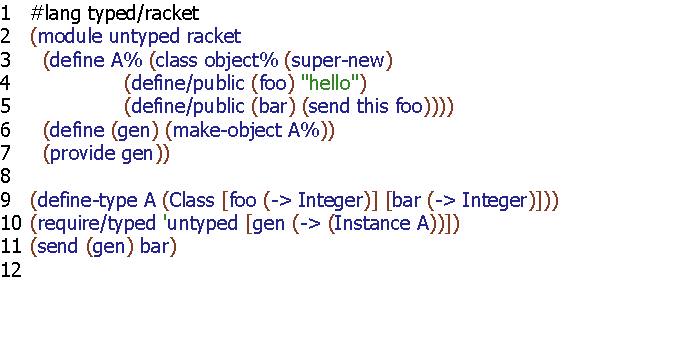
\includegraphics[scale=.7]{figures/internal.pdf}&\hspace{-2cm}
\begin{minipage}{.5\textwidth}
\vspace{-4.3cm}
\tiny
\begin{lstlisting}[basicstyle=\scriptsize\ttfamily]
foo: broke its own contract
  promised: Integer
  produced: "hello"
  in: the foo method in
      the range of
      (->
       (object/c
        (bar (-> any/c Integer))
        (foo (-> any/c Integer))))
  contract from: (interface for gen)
  contract on: gen
  blaming: (interface for gen)
\end{lstlisting}
\end{minipage}
\end{tabular}
\caption{Typed Racket ensures that internal untyped calls respect external types}
\label{fig:arktex3}
\end{figure}

This issue is illustrated in figure~\ref{fig:intbeh2}, where the source program
initially requires \n to take \xt{A} and return \xt{A}, then requires it to take
and return \xt{B}. If we lift the methods up verbatim (adding only the trivial
casts), then we end up with a type-incorrect wrapper. As a result, we have to
dynamically insert casts inside of the lifted method bodies, ensuring that they
remain type correct in the wrapper class. This operation is depicted in detail
in the appendix.


\begin{figure}[!ht]
\begin{tabular}{l@{\hspace{0.05\textwidth}}l@{\hspace{0.05\textwidth}}l}
\begin{minipage}{0.3\textwidth}
\begin{lstlisting}
class A {n(x:*):*{x}}
class B {m(x:*):*{x}}
class C { 
  m(x:A):A { 
    this.n(x) }
  n(x:A):A { x }}
class D { 
  m(x:A):A { x }
  n(x:B):B { x }}
(<D>new C()).m(
  new C())
\end{lstlisting}
\end{minipage}
&
\begin{minipage}{0.25\textwidth}
\begin{lstlisting}
class DW {
  that : C
  

  m(x:A):A { 
    this.n(x) }

  n(x:B):B { 
    (*@\hspace{-1.5mm}\BehStart\hspace{-1.5mm}@*)B(*@\BehEnd@*)(*@\ShaStart\hspace{-1.5mm}@*)B(*@\ShaEnd\hspace{0mm}@*)
    (*@\hspace{-0.5mm}\BehStart\hspace{-1.5mm}@*)A(*@\BehEnd@*)(*@\ShaStart\hspace{-1.5mm}@*)A(*@\ShaEnd\hspace{0mm}@*)x }
}
\end{lstlisting}
\end{minipage} &
\begin{minipage}{0.3\textwidth}
\begin{lstlisting}
class DW {
  that : C

  m(x:A):A { 
    (*@\hspace{-0.5mm}\BehStart\hspace{-1.5mm}@*)A(*@\BehEnd@*)(*@\ShaStart\hspace{-1.5mm}@*)A(*@\ShaEnd\hspace{0mm}@*)this.n(
      (*@\hspace{-0.5mm}\BehStart\hspace{-1.5mm}@*)B(*@\BehEnd@*)(*@\ShaStart\hspace{-1.5mm}@*)B(*@\ShaEnd\hspace{0mm}@*)x) }

  n(x:B):B { 
    (*@\hspace{-1.5mm}\BehStart\hspace{-1.5mm}@*)B(*@\BehEnd@*)(*@\ShaStart\hspace{-1.5mm}@*)B(*@\ShaEnd\hspace{0mm}@*)
      (*@\hspace{-0.5mm}\BehStart\hspace{-1.5mm}@*)A(*@\BehEnd@*)(*@\ShaStart\hspace{-1.5mm}@*)A(*@\ShaEnd\hspace{0mm}@*)x }
}
\end{lstlisting}
\end{minipage} \\
Source & Type-incorrect & Type-corrected
\end{tabular}
\caption{Wrapper generation}
\label{fig:intbeh2}
\end{figure}

The other major concern when designing a wrapper-based protection system for 
objects is that losing methods is a real possibility. If a wrapper zealously 
enforces its type, then it will not wrap methods that do not appear on its type,
which can then be lost to later untyped or more-typed code that is given that
wrapper. 

%%%%%%%%%%%%%%%%% EXAMPLE  <C><D>new C %%%%%%%%%%%%%%%%%%%%%%%%%%%%%%%%%%%%
\begin{figure}[h!]
\footnotesize
\begin{tabular}{ll}\begin{minipage}{6cm}
\[\begin{array}{l}
\class ~\C~ \{\\
\SP  \Mdef\m\x\E\E\x\\
\SP  \Mdef\mp\x\E\E\x\\
\}\\[2mm]
\class ~\EMxt{CtoD}~ \{\\
\SP  \Fdef\that\C\\
\SP  \Mdef \m\x\any\any{\BehCast\any{\ShaCast\any{\BehCast\E{\ShaCast\E\x}}}}\\
\SP  \Mdef \mp\x\E\E{\x}\\
\}\\
\end{array}\]
\end{minipage}
&
\begin{minipage}{5cm}
\[\begin{array}{l}
\class ~\D~ \{\\
\SP  \Mdef\m\x\any\any\x\\
\}
\\
\\[2mm]
\class ~\EMxt{CtoDtoC}~ \{\\
\SP  \Fdef\that{\EMxt{CtoD}}\\
\SP  \HT{\m(\HT\x\E)}{\E}\;\{\BehCast\E{\ShaCast\E{\BehCast\any{\ShaCast\any{}}}} \\
\SP ~~~~{\BehCast\E{\ShaCast\E{\BehCast\any{\ShaCast\any\x}}}}\}\\
\SP  \Mdef\mp\x\E\E{ \BehCast\E{\ShaCast\E{\BehCast\E{\ShaCast\E\x}}}}\\
\SP  \Mdef\mp\x\any\any{ \BehCast\any{\Call\this\mp{\BehCast\E{\ShaCast\E{\x}}}}}\\
\}\\
\end{array}\]
\end{minipage}
\end{tabular}
\caption{Wrapper classes generated by \BehCast\C{(\BehCast\D{\New\C{}})}}
\label{ctod}
\end{figure}

Our approach avoids this by inserting ``passthrough'' methods that retain their
original types and behaviors into the output wrappers, as illustrated in
figure~\ref{ctod}, where we make a \C into a \D and then back again. When we
reduce the set of required methods by casting a \C to a \D, we retain the method
\mp by adding it to the output class. Notably, this operation preserves existing
subtyping relationships, as the generated wrappers only appear as values, and
the operation only adds additional methods.

The Typed Racket translation demonstrates some of the key issues inherent in a
wrapper-based system, where wrapper-inserting casts build up very quickly
internally, leading to the potential for a wrapper explosion, as previously noted
by Takikawa et al~\cite{practical-gt}, a point that is further highlighted by
the number of casts inserted into the wrappers, even if unnecessary casts are
then removed.


%%%%%%%%%%%%%%%%%%%%%%%%%%%%%%%%%%%%%%%%%%%%%%%%%%%%%%%%%%%%%%%%%%%%%%%%


\subsection{Monotonic Python}

On the surface, the monotonic and transient semantics are very similar, both
semantics requires consistency, but consistency is substantially more
important within the monotonic semantics.

\begin{mathpar}
\IRule{C1}{\tmeet\t\tp\cdot\K = \tpp\,\Kp}{\consistent\K{\t}{\tp}} 
\end{mathpar}

Consistency is effectively the idea that two types do not
contradict one another. For example, the types \xt{int} and \any are
consistent, but the types \xt{int} and \xt{string} are not as no member of
one could be in the other.

The consistency operator ($\sim$) in our formal system is implemented using the concept of meet described
by the \texttt{tmeet} function. The \xt{tmeet} function finds the common type 
between two given types, which if a common type exists, it implies that consistency holds between 
the two given types. Using the earlier example, the meet between \xt{int} and \any would be \xt{int}, 
as \xt{int} is the more restrictive of the two types. In effect, the \texttt{tmeet} function fulfills the 
same purpose as the $\sqcap$ operator in~\cite{Siek2015}. 

\begin{figure}[!ht]
\begin{tabular}{EEEEEVEV}
\texttt{tmeet(}
& \texttt{A}
  & \texttt{,}
  \texttt{B}
  & \texttt{,}
  $\cdot$
  & \texttt{,}
  &
\begin{lstlisting}
class A {
   m(x: *): A {this}}

class B {
   m(x: B): * {this}}
\end{lstlisting}    
& 
\texttt{) = C,}
  &
\begin{lstlisting}
class A { ... }
class B { ... }
class C {
  m(x: B): A {this}
}
\end{lstlisting}    
\end{tabular}
\caption{Simple example of \texttt{tmeet}}
\label{fig:tmeet_ex}
\end{figure}

Consider the simple example in figure~\ref{fig:tmeet_ex}, where we compute
the meet of \texttt{A} and \texttt{B}, both classes have the same function,
but with alternating the typing.  The function in class \texttt{A} has the
return type typed, whereas the function in class \texttt{B} has the argument
typed.  Calling the \texttt{tmeet} function on \texttt{A} and \texttt{B}
will compute the new type \texttt{C}, whose method have will have typed
argument and return type. The \texttt{tmeet} function will be described in
more detail once the monotonic cast semantic is presented.

\begin{figure}[h!]
\colorbox{vlightgray}{
\begin{minipage}{0.25\textwidth}
\large \textbf{Static Typing}
\vspace{-2.5mm}
\begin{mathpar}
\IRule{W10}{
  \EnvType \Env\s\K\e\tp
}{
  \EnvType \Env\s\K{\MonCast\t\e}\t
}
\end{mathpar}
\end{minipage}
}
\hspace{0.08cm}
\colorbox{vlightgray}{
\begin{minipage}{0.6\textwidth}
\begin{tabular}{l@{}l@{~}l@{~}l}
\multicolumn{4}{l}{ \large \textbf{Dynamics} } \\
\CondRule{E11}{  %% Monotonic cast  
  \moncast \a\t\s\K  \Kp\ap\sp    
}{    
  \ReduceA  \K{\MonCast \t\a}\s \Kp\ap\sp   
} \\
\multicolumn{4}{l}{\EE ::= \ldots \B \MonCast\t\EE }
\end{tabular}
\end{minipage}
}
\caption{Monotonic cast static and dynamic rules}
\label{fig:monrules}
\end{figure}

Similar to the behavioural semantics, the monotonic semantics is implemented to the core of \kafka
as a cast extension. For an expression \e and type \t, we write \MonCast\t\a to depict the monotonic cast.
Figure \ref{fig:monrules} presents the typing and semantics rules for the monotonic cast.

\begin{figure}[!ht]
\begin{mathpar}
\IRule{PT}{
  {\classtrans{\K}{\K}{\K'}} \\ \GenCast{\K}{\cdot}{\e}{\ep}{\t} 
}{\progtrans{\e~\K}{\e'~{\K'}}}

\IRule{MCT1}{
  \D \text{ fresh}\\
  \k = \classgen{\C,\getmds\C\K,{\classoff\C\K},{\classoff\C\K},\D,\K}
}{
  \monowrap{\C}{\K} = \D~\k
}

\IRule{MCT2}{
}{
  \monowrap{\any}{\K} = \any
}

\IRule{CR1}{ 
  \b{\methtrans \K\C\md{\md'}{\K_m}} \\
  \classtrans \K\Kp\Kpp \\
  \b{\monowrap\t\Kpp = \tp~\Kppp}
}{
   \classtrans \K{\Class \C{\b{\Ftype\f\t}}{\b\md}~\Kp}{\Class \C {\b{\Ftype\f\tp}}{\b{\md'}}~\Kpp~\K_m~\b{\Kppp}}}

\IRule{CR2}{ 
}{
  \classtrans \K\cdot\cdot
}

\IRule{MT}{
  \AnaCastMono \K{\HT\this\C~\HT\x\t}\e\ep\tp{\K_1} \\
  \monowrap{\t_1}\K = \t_2~\K_2 \\
  \monowrap{\tp_1}\K = \tp_2~\K_3
}{
  \methtrans \K\C{\Mdef\m\x{\t_1}{\tp_1}\e}{\Mdef\m\x{\t_2}{\tp_2}\ep}{\K_1~\K_2~\K_3}
}
\end{mathpar}
\caption{Monotonic translation for program, class, and method}
\label{fig:mono-trans1}
\end{figure}


The translation from the monotonic surface language to \kafka begins 
in figure \ref{fig:mono-trans1}. The rule \RuleRef{PT} translates 
monotonic programs, \RuleRef{CR1} and \RuleRef{CR2} translates monotonic class,
and \RuleRef{MT} translates monotonic methods. In the \RuleRef{MT} 
and \RuleRef{CR1} rules, we are actively replacing every type the user wrote with ones generated by the 
\xt{monWrap} function. The details of the \xt{monWrap} function will be 
discussed later, but for the purposes of the translation, we can assume that the
\xt{monWrap} function will replace every typed function with an untyped one unless
there are no \any types transitively contained within the function's argument.

\begin{figure}[!ht]
\begin{mathpar}
\IRule{MOS1}{\HasType{\E}\x\t}{\GenCastMono{\K}\E\x\x\t{}}

\IRule[width=30em]{MOS2}{
    \GenCastMono\K\Env{\e_1}{\e_3}{\C}{\K_1} \\ \n(\b{\t_1}):\t_2 \in \classoff\C\K \\ \statictype{\src{\t_1}}{\src\K}{\cdot} \vee \n=\f \\ \b{\AnaCastMono\K\Env{\e_2}{\e_4}{\t_1}{\K_2}}
}{
    \GenCastMono\K\Env{\Call{\e_1}\n{\b{\e_2}}}{\Call{\e_3}\n{\b{\e_4}}}{\t_2}{\K_1~\b{\K_2}}
}

\IRule[width=30em]{MOS3}{
    \GenCastMono\K\Env{\e_1}{\e_3}{\C}{\K_1} \\ \m({\t_1}):\t_2 \in \classoff\C\K \\ \lnot\statictype{\t_1}{\K}{\cdot} \\ \b{\AnaCastMono\K\Env{\e_2}{\e_4}{\t_1}{\K_2}}
}{
    \GenCastMono\K\Env{\Call{\e_1}\m{{\e_2}}}{\DynCall{(\MonCast\any\e_3)}\m{\MonCast\any{\e_4}}}{\t_2}{\K_1~\b{\K_2}}
}

\IRule{MOS4}{
    \AnaCastMono\K\Env{\e_1}{\e_3}{\any}{\K_1} \\ {\AnaCastMono\K\Env{\e_2}{\e_4}{\any}{\K_2}}
}{
    \GenCastMono\K\Env{\DynCall{\e_1}\m{{\e_2}}}{\DynCall{\e_3}\m{{\e_4}}}{\any}{\K_1~\K_2}
}

\IRule{MOS5}{
  \b{\AnaCastMono{\K}\E{\e_1}{\e_2}\t{\K}} \\ 
  \Class \C {\b{\Ftype\f\t}} {\b{\md}} \\
  \D~\text{fresh} \\
  \k = \classgen{\C,\getmds\C\K,\classoff\C\K,\classoff\C\K,\D,\K} \\
  }{\GenCastMono\K\Env{\New\C{\b{\e_1}}}{\New\D{\New\C{\b{\e_2}}}}{\C}{\K~\k}}
\end{mathpar}
\caption{Monotonic translation for expressions}
\label{fig:mono-trans2}
\end{figure}

The expression translations are presented in figure \ref{fig:mono-trans2}. 
The \texttt{static} function states whether a type contains only typed methods.
The rule \RuleRef{MOS2} translates typed methods, \RuleRef{MOS2} translate methods that are not purely typed.
\RuleRef{MOS4} translate untyped methods, \RuleRef{MOS2} translate object creation.
The purpose of the \xt{monWrap} function is further evidenced as the 
handling of calls to methods need to appropriately casted if the typing nature is unclear.

\begin{figure}[!ht]
\begin{mathpar}
\IRule{MOA1}{
  \GenCastMono\K\Env\e\ep\tp\K \\
  \K \vdash \tp \Sub \t
}{
  \AnaCastMono\K\Env\e\ep\t\K
}

\IRule{MOA2}{
  \GenCastMono\K\Env\e\ep\tp\K \\
  \consistent\K\t\tp
}{
  \AnaCastMono\K\Env\e{\MonCast\t\ep}\t\K
}
\end{mathpar}

\caption{Monotonic translation for bidirectional expressions}
\label{fig:mono-trans3}
\end{figure}

Monotonic has identical analytical cast insertion to the transient system,
combining subtyping with consistency, seen in in figure \ref{fig:mono-trans3},
which allow use the of either subtyping or consistency in type coercions

\subsection{Monotonic Casts}

The monotonic cast \MonCast\C\a imposes the type \C onto the object
at \a and every object transitively reachable from \a. The motivation 
for this cast comes from maintaining the
type correctness of every reference in the program~\cite{Siek2015}.

\begin{figure}[h!]
\begin{tabular}{ll}
\begin{minipage}[b]{4cm}
\lstset{framesep=4pt}
\begin{lstlisting}
class C { f : * }
class D { 
  m (x:*):* {x}
}

d:* = new D()
a:* = new C(d)
[heap snapshot 1]

class E { f : F }
class F { 
  m (x:E):E {x}
}

e:E = <E>a
[heap snapshot 2]
d.m(d)
\end{lstlisting}
\vspace{-9.2em}
\end{minipage}
&
\begin{tabular}{l}
\\
Heap snapshot 1: \\
\begin{minipage}{8cm}
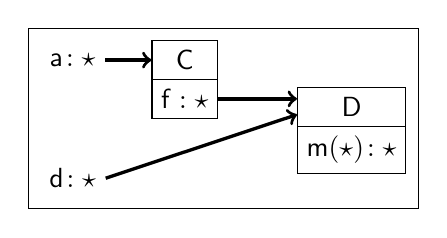
\begin{tikzpicture}[framed,my shape/.style={
rectangle split, rectangle split parts=#1, draw, anchor=text east}]
\node (ref) at (0,0) {$\HT\a\any$};
\node (refb) at (0,-1.5) {$\HT{\xt{d}}\any$};

\node (C1) [my shape=2,right of=ref, anchor = text west]
{\C\nodepart{two}$\f : \any$};

\node (D1) [my shape=2,right=of C1.two east, anchor=text west,shift={(0,-.1)}]
{\D\nodepart{two}$\Mtype\m\any\any$};

\draw[->,very thick] (ref.east) -> (C1.text west);
\draw[->,very thick] (refb.east) -> ($(D1.text west)+(0,-.1)$);
\draw[->,very thick] (C1.two east) -> ($(D1.text west)+(0,.1)$);
\end{tikzpicture}
\end{minipage}\\
\\
Heap snapshot 2: \\
\begin{minipage}{8cm}
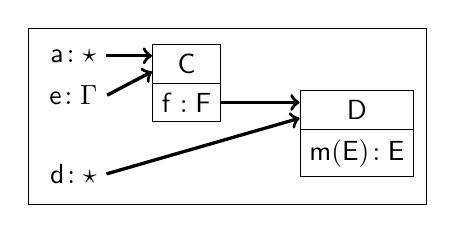
\begin{tikzpicture}[framed,my shape/.style={
rectangle split, rectangle split parts=#1, draw, anchor=text east}]
\node (ref) at (0,0) {$\HT\a\any$};
\node (refb) at (0,-1.5) {$\HT{\xt{d}}\any$};
\node (refe) at (0,-.5) {$\HT{\xt{e}}\E$};

\node (C1) [my shape=2,right of=ref, anchor = text west,shift={(0,-.1)}]
{\C\nodepart{two}$\f : \xt{F}$};

\node (D1) [my shape=2,right=of C1.two east, anchor=text west,shift={(0,-.1)}]
{\D\nodepart{two}$\Mtype\m{\xt{E}}{\xt{E}}$};

\draw[->,very thick] (ref.east) -> ($(C1.text west)+(0,.1)$);
\draw[->,very thick] (refb.east) -> ($(D1.text west)+(0,-.1)$);
\draw[->,very thick] (refe.east) -> ($(C1.text west)+(0,-.1)$);
\draw[->,very thick] (C1.two east) -> ($(D1.text west)+(0,.1)$);
\end{tikzpicture}
\end{minipage}
\end{tabular}
\vspace{1em}
\end{tabular}
\caption{Execution under the monotonic semantics}
\label{fig:mono_ex1}
\end{figure}

Figure~\ref{fig:mono_ex1} presents an example of the monotonic cast. 
A new instance of class \D is created, then an instance of class \C 
is created pointing to it. As shown by heap snapshot 1, 
the field \f in \C has type \any, and the method \m in \D has dynamic 
argument and return type. Classes \E and \xt{F} are introduced and they are structurally 
identical to \C and \D, but with specific types for their fields and methods. 
When the instance of class \C referenced by \a is casted to \E, 
the monotonic semantics will ensure any access to field \f or method \m from 
anywhere in the program will follow the type invariants asserted by class \E.

However, as shown in heap snapshot 2, the reference \xt{d} still refer to 
the instance of \D, from earlier, and \xt{d}
does not know the existence of the new invariant applied to class \D. Despite being
typed \any, when \xt{d} try to invoke method \m on the apparently dynamic 
object, a cast failure will occur. The monotonic semantics ensures that the
provided argument must be of type \E. 

This example highlights the need for the monotonic cast semantics to be generative.
In order to guarantee the type correctness of all references, monotonic has to generate guards
that check the argument and return type of every method, and the
type of any field set, ensuring that they maintain consistency with the 
maximally static type. Additionally, monotonic ensures that 
prior references respect future type invariants by performing an in-place update
of any object whose type is altered by the cast.

In the extreme case, a single cast would retype every object in the heap. 
In order to prevent the pathological case, the monotonic casts only modify the heap
if the target \C has fewer occurrences of \any than the original type of the
object at \a (and transitively so for types appearing in \t and reachable
from \a).  When a type \C does not have any occurrence of the dynamic type,
denoted by \statictype\C\K\V, the monotonic casts will leave the object and the
heap unchanged.

%TODO Do we need this text describing monotonic correctness property
% The key challenge of monotonic is for every class typed reference to 
% preserve correctness after the monotonic cast. 
% To accomplish this property, the monotonic cast ensure two properties:
% \begin{itemize}
% \item The values that currently exist cannot violate any of the types
%   that point to them. Casting needs to recursively ensure that all values
%   referred to by the current object are of the claimed type.
% \item Functions can not be called with or return values that violate any of
%   the types that they are referred to. The behaviour of the class needs
%   to check that its types are not violated by lesser-typed call sites.
% \end{itemize}
% The second property is strongly reminiscent of the behavioural semantics,
% though with the interesting caveat that all method invocations 
% must follow the typed calling conventions, rather
% than just the ones that inherit this particular type assertion.

The monotonic cast semantics in \kafka cannot be implemented using the  
in-place replacement technique\cite{Siek2015}. In order to ensure the
type of a field is respected, the monotonic cast will insert a setter method
checking the value given to it against the type of the field, when
a lesser-typed call site is used to set the field. However, \kafka prohibits
the explicit existence of a field and its getter and setter methods.
As a field and its getter and setter method must be in-sync at all times.
This means the monotonic cast semantics is implemented in \kafka by adding a 
single wrapper over each object, similar to the ``identity preserving membrane''
described in \cite{keil_et_al:DARTS:2015:5511}. The wrappers will preserve the
externally-facing interface (up to a point) and the relations between classes,
while ensuring all properties in the monotonic system are guaranteed.

As a result of generating the wrappers (and the static translation), the simple example 
shown in figure~\ref{fig:mono_ex1} does not correctly exhibit the correct behavior of the 
monotonic semantics in \kafka, instead the example presented in figure~\ref{fig:mono_ex2}
depicts the correct semantics for \kafka's monotonic cast.
For compactness, the class definitions in figure~\ref{fig:mono_ex1}, and the class definitions that will be generated but
not appear in the dynamic execution have been elide.

\begin{figure}[h!]
\centering
\begin{minipage}{5cm}
\begin{tabular}{l}
Translated Program:\\
\begin{lstlisting}
d:* = new DW(new D())
a:* = new CW(new C(d))
[heap snapshot 1]
e:E = <E>a
[heap snapshot 2]
d.m(d)
\end{lstlisting}
\end{tabular}
\end{minipage}
\begin{tabular}{@{}l@{\hspace{3mm}}l@{}}
Class \C Wrappers: & Class \D Wrappers: \\
\begin{minipage}{7cm}
\begin{lstlisting}
class CW { 
  that : C
  f():* { <*>this.that().f() }
  f(x:*):* { 
    <*>this.that().f(<*>x)}
}
class ECW {
  that : C
  f():* { <*><FW>this.that.f() }
  f(x:*):* {
    <*><FW>this.that().f(<*><FW>x)}
}
\end{lstlisting}
\end{minipage}
&
\begin{minipage}{7cm}
\begin{lstlisting}
class DW { 
  that : D
  m (x:*):* { <*><*>x }
}



class FDW {
  that : D
  m(x:*):* { <*><EW><*><EW>x }
  m(x:EW):EW { <EW><*><EW>x }
}
\end{lstlisting}
\end{minipage}
\\
Heap snapshot 1: & 
Heap snapshot 2: \\
\begin{minipage}{7cm}
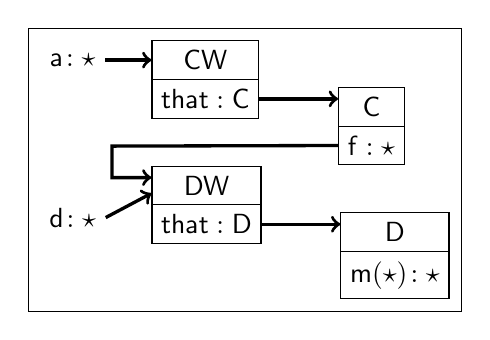
\begin{tikzpicture}[framed,my shape/.style={
rectangle split, rectangle split parts=#1, draw, anchor=text east}]
\node (ref) at (0,0) {$\HT\a\any$};
\node (refb) at (0,-2) {$\HT{\xt{d}}\any$};

\node (C1) [my shape=2,right of=ref, anchor = text west]
{\xt{CW}\nodepart{two}$\that : \C$};

\node (C2) [my shape=2,right=of C1.two east, anchor=text west,shift={(0,-.1)}]
{\xt{C}\nodepart{two}$\f : \any$};

\node (D1) [my shape=2,below=of C1.two west, anchor=text west,shift={(0,-.1)}]
{\xt{DW}\nodepart{two}$\that : \D$};

\node (D2) [my shape=2,right=of D1.two east, anchor=text west,shift={(0,-.1)}]
{\xt{D}\nodepart{two}$\Mtype\m\any\any$};

\draw[->,very thick] (ref.east) -> (C1.text west);
\draw[->,very thick] (refb.east) -> ($(D1.text west)+(0,-.1)$);
\draw[->,very thick] (C1.two east) -> ($(C2.text west)+(0,.1)$);
\draw[->,very thick] (C2.two west) -- ($(D1.text west) + (-0.5,0.5)$) -- ($(D1.text west) + (-0.5,.1)$) -> ($(D1.text west)+(0,.1)$);
\draw[->,very thick] (D1.two east) -> ($(D2.text west) + (0,.1)$);
\end{tikzpicture}
\end{minipage} &
\begin{minipage}{7cm}
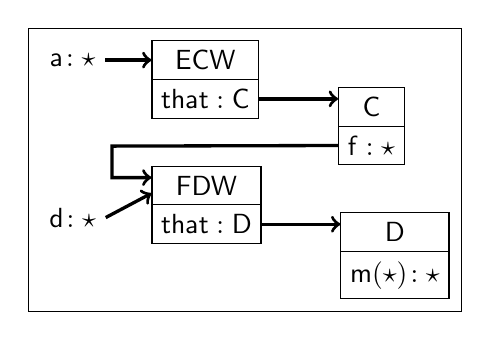
\begin{tikzpicture}[framed,my shape/.style={
rectangle split, rectangle split parts=#1, draw, anchor=text east}]
\node (ref) at (0,0) {$\HT\a\any$};
\node (refb) at (0,-2) {$\HT{\xt{d}}\any$};

\node (C1) [my shape=2,right of=ref, anchor = text west]
{\xt{ECW}\nodepart{two}$\that : \C$};

\node (C2) [my shape=2,right=of C1.two east, anchor=text west,shift={(0,-.1)}]
{\xt{C}\nodepart{two}$\f : \any$};

\node (D1) [my shape=2,below=of C1.two west, anchor=text west,shift={(0,-.1)}]
{\xt{FDW}\nodepart{two}$\that : \D$};

\node (D2) [my shape=2,right=of D1.two east, anchor=text west,shift={(0,-.1)}]
{\xt{D}\nodepart{two}$\Mtype\m\any\any$};

\draw[->,very thick] (ref.east) -> (C1.text west);
\draw[->,very thick] (refb.east) -> ($(D1.text west)+(0,-.1)$);
\draw[->,very thick] (C1.two east) -> ($(C2.text west)+(0,.1)$);
\draw[->,very thick] (C2.two west) -- ($(D1.text west) + (-0.5,0.5)$) -- ($(D1.text west) + (-0.5,.1)$) -> ($(D1.text west)+(0,.1)$);
\draw[->,very thick] (D1.two east) -> ($(D2.text west) + (0,.1)$);
\end{tikzpicture}
\end{minipage}
\end{tabular}
\caption{Execution under the monotonic semantics}
\label{fig:mono_ex2}
\end{figure}

Figure~\ref{fig:mono_ex2} aims to illustrate the nature of the monotonic wrappers. 
In this example, the state of the heap is highlighted
at two discrete times, before and after the cast of the reference \a to
the type \xt{E}. The wrapper \xt{CW} and \xt{DW} is associated with enforcing 
the class \C and \D, respectively, and wraps over an underlying object of 
known type, enforcing its type guarantees.

The monotonic semantics will lift the method bodies into wrapper classes, as seen in
the Typed Racket semantics but for different reasons. While Typed Racket
needs to enforce the observed type on an underlying untyped object. The
monotonic semantics need the combination of the wrapper and underlying object 
to act as if they are exactly the monotonically specified type. 
The result of this can be seen in the translation above for \m.

A notable behavior of the monotonic semantics illustrated in figure~\ref{fig:mono_ex2}
is the erasure on every call site for \m, with the exception of the final definition in \xt{FDW}. 
Under the monotonic semantics, every call site with some untyped component
will be adjusted further, ensuring any partially typed call may be invalidated in the future. 
As a consequence, every call, even to a superficially typed call site (one with an argument
type that may contain a \any deeply embedded in the type), must be treated as an untyped call site.

In the monotonic semantics, if we encounter a cast on a reference, that cast needs to be
enforced upon that reference for the rest of its lifetime. \kafka's monotonic
cast semantics handles this by taking the previously-existing type on the object,
computing the meet of that old type and the new type, producing a new
wrapper for the object that replaces the previous wrapper. The wrappers \xt{ECW} and \xt{FDW}
are created when \a is casted to \xt{E}.
To ensure that types for fields are respected, we take a conservative approach, 
as seen in \xt{ECW}. When a field on an underlying object is set, we first cast
it to the required type (in this case \xt{FW}). Then a further $\star$ cast is applied 
to the type of the underlying storage cell. For retrieving values, we reverse this process.

The result wrappers are sometimes overly conservative. From the semantics of the meet operation, we
know that the first cast to the protected type is sufficient to ensure 
compatibility with the underlying memory cell type, and we also know that casting
to the required type before returning is ignoring the heap consistency invariant 
that monotonic provides, allowing for casts on retrieval to be ignored. However,
the \kafka type system does not allow us to make either of these shortcuts while
still retaining semantic correctness, and as a result, we are forced to double 
up on the casts over the getter and setter methods, as seen in \xt{ECW}.
Another point of interest is the alteration happening in \xt{FDW}. When the class \xt{D}
is specialized to \xt{F}, several additional casts
are inserted, as well as a wholly new call site for \m. This new
call site is fully typed, despite previously stating that we could not add any 
typed call sites as they might be changed in the future.
In this case, we are able to insert the additional static call site because we 
know that \xt{E} will not be able to be further altered under the monotonic 
semantics, as \xt{E} and every type referenced from it have no instances of the
type \any in them, which might be altered in the future by another monotonic
cast.

%\begin{figure}
%\begin{tabular}{ccc}
%\begin{minipage}
%\begin{lstlisting}
%class A { f:* }
%class B { f:* f2:* }
%class C { f:D }
%class D { f:E f2:* }
%class E { f:E f2:E }
%\end{lstlisting}
%&
%\begin{tikzpicture}
%\node (a) at (0,0) {\a : \any};
%\node (a1) [below=of a] {\ap : \any};
%\end{tikzpicture}
%&
%\end{tabular}
%\end{figure}

\begin{figure}
\begin{mathpar}
\IRule{CM}{
  \retype \a\t\cdot\s\K = \S~\Kp\\
  \spec {\Dom\S} \S\s\Kp = \sp~\Kpp
}{
  \moncast \a\t\s\K \Kpp \sp\\
}
\end{mathpar}
\caption{Monotonic cast semantics}
\label{fig:mono_sem}
\end{figure}

The monotonic cast semantics is formally defined by the \xt{moncast} rule, 
which takes the address of the cast object \a, a target type \t, the current heap \s, 
and class table \K, and gives an update heap \sp and an updated class table \Kp.

The functionality of the \xt{moncast} rule is broken into two functions.
The first function (\xt{retype}) identities the correct target type for every object affect by
the monotonic cast, storing the gathered objects and their types in the meta-variable \S, 
a mapping from addresses to classes, creating a blueprint for the sub-heap affected 
by the monotonic cast. The second function (\xt{spec}) updates the heap and class table with the
objects and types listed in \S.

\begin{figure}[!ht]
\opdef{
  $\tmeet{\t}{\tp}\P\K = \tpp\,\Kp$
}{
}
\begin{align*}
\P &::= \cdot \B \Map\P{\Bind{(\C,\D)}\E}
\end{align*}
\begin{mathpar}
\IRule{TM1}{ }{\tmeet\C\any\P\K = \C\,\K}

\IRule{TM2}{ }{\tmeet\any\C\P\K = \C\,\K}

\IRule{TM3}{ }{\tmeet\t\t\P\K = \t\,\K}

\IRule{TM4}{
  \fresh\E\\
  (\C,\D) \not\in\P \\
  \Pp = \Map\P{\Bind{(\C,\D)}\E} \\
  \mtypes\C\K = {\b\mt}\\
  \mtypes\D\K = {\b\mtp}\\
  \mmeet{\b\mt}{\b\mtp}\Pp\K = \b\mtpp\,\Kp\\
  \Kpp = \Kp~\typegen{\b\mtpp}\E\\
}{
    \tmeet\C\D\P\K = \E\,\Kpp
}

\IRule{TM5}{
    \P(\C,\D) = \E
}{
    \tmeet\C\D\P\K = \E\,\K
}
\end{mathpar}
\caption{The \texttt{tmeet} function}
\label{fig:tmeet_fun}
\end{figure}

The \xt{retype} function utilizes the meet operation in determining the correct
casting type for every object transitively reachable from the cast object. 
Figure~\ref{fig:tmeet_fun} presents the \xt{tmeet} function, which computes
the meet between two types. The \xt{tmeet} function takes four arguments,
the two types being meet, a meta-variable \P, and the class table \K. 
The meta-variable \P denotes a list of mappings 
from a pair of types to the type produced from their meet. The rules
\RuleRef{TM1} and \RuleRef{TM2} describe the meet of a $\star$. The rule
\RuleRef{TM3} describes the identity meet. The rule \RuleRef{TM5} describes
the recursive case of our meet operation. 
The rule \RuleRef{TM4} retrieves the method typing for each type, computes 
the meet of those method typing (by calling an auxiliary function (\xt{mmeet}),
and updates the class table with a new class containing the method typing 
produced from the meet.

\begin{figure}[!ht]
\begin{tabular}{l@{}l@{}l@{}l@{}l@{\hspace{1.5mm}}l@{\hspace{1mm}}l@{}l}
\texttt{tmeet(}
& \texttt{A}
  & \texttt{,}
  \texttt{B}
  & \texttt{,}
  $\cdot$
  & \texttt{,}
  &
  \begin{minipage}{4.3cm}
    \begin{lstlisting}
class A {
   m(x: A): A {this}}

class B {
   m(x: B): B {this}}
      \end{lstlisting}    
  \end{minipage}
& 
\texttt{) = E,}
  &
  \begin{minipage}{4.3cm}
    \begin{lstlisting}
class A { ... }
class B { ... }
class E {
  m(x: E): E {this}
}
    \end{lstlisting}    
  \end{minipage}
\end{tabular}
\caption{\texttt{tmeet} example over recursive classes}
\label{fig:tmeet_rec_ex}
\end{figure}

The meta-variable \P becomes crucial when considering the example
in figure~\ref{fig:tmeet_rec_ex}, where the meet  of \xt{A} and \xt{B}
recursively depends on the meet of \xt{A} and \xt{B}. If we proceeded naively,
without \P, \RuleRef{TM4} would invoke \RuleRef{TM4} again to compute the meet
of the arguments to \m. We use \P and \RuleRef{TM5} to avoid this.

\RuleRef{TM4} invokes \xt{mmeet} with an enriched \P, in much the same manner
that the subtyping relation does, inserting the future result of the meet of
\xt{A} and \xt{B} (\xt{E} in this example) into \P, will then
be used by \RuleRef{TM5} to terminate the recursion.

\section{Conclusion}

Gradual typing is no longer simply a popular research topic in academia.
Real world applications are being written with gradual typing like
languages.  Types are progressively being introduced into existing untyped
applications.  It's the responsibility of language researchers to present a
clear understanding of each viable gradual typing idiom available.

We have presented \kafka, a formal language that serves as the foundation
for constructing five existing gradual typing systems: Typescript, Thorn,
Transient, Type Racket, and Monotonic. \kafka offers the opportunity for
comparing and contrasting these gradual typing systems within an unified
framework. The translations to \kafka for each gradual typing system
highlights the essences which makes each system unique.

From \kafka, we have developed a better understanding for the lightweight
nature of TypeScript, the restrictiveness of Thorn, the excessiveness of the
wrappers generated by Type Racket, the safety guarantees of Transient, and
the complexity and dynamic nature of Monotonic.  However, the aim of this
paper is not only to provide a deeper understanding for each individual
gradual typing system, but a road map for the direction of gradual typing in
general.


\clearpage

\bibliographystyle{unsrturl}
\bibliography{../bib/jv,../bib/all,../bib/ben}

\clearpage

\appendix
%%%%%%%%%%%%%%%%%%%%%%%%%%%%%%%%%%%%%%%%%%%%%%%%%%%%%%%%%%%%%%%%%%%%%%%%%%%%%%
%%%%%%%%%%%%%%%%%%%%%%%%%%%%%%%%%%%%%%%%%%%%%%%%%%%%%%%%%%%%%%%%%%%%%%%%%%%%%%
\section{Auxiliary Definitions for \kafka}%%%%%%%%%%%%%%%%%%%%%%%%%%%%%%%%%%%%
%%%%%%%%%%%%%%%%%%%%%%%%%%%%%%%%%%%%%%%%%%%%%%%%%%%%%%%%%%%%%%%%%%%%%%%%%%%%%%
%%%%%%%%%%%%%%%%%%%%%%%%%%%%%%%%%%%%%%%%%%%%%%%%%%%%%%%%%%%%%%%%%%%%%%%%%%%%%%

\subsection{Subtyping}

The structural subtype relation, written \StrSub\M\K\t\tp, asserts that \t
is a subtype of \tp in the environment \M composing a set of subtype relations and
a class table \K.   The set of subtype relations can be omitted if its empty.

~\\

\opdef{\StrSub\M\K\t\tp}{\t is a subtype of \tp}
\begin{mathpar}
\IRule{SRef}{
}{
 \StrSub\M\K \t \t
}

\IRule{SAss}{
\C \Sub \D \in \M
}{
 \StrSub \M\K \C \D
}

\IRule{SRec}{
 \M' = \M~\C\Sub\D\\
\mt \in \classoff\D\K \implies \mtp \in \classoff\C\K ~.~ \StrSub{\M'}\K\mt{\mtp}
}{
 \StrSub \M\K \C \D 
}
\end{mathpar}

\begin{mathpar}
\IRule{SMet}{
  \StrSub \M\K {\t[1]} {\t[2]} \\
  \StrSub \M\K {\tp[2]} {\tp[1]}
}{
 \StrSub \M\K {\Mtype\m{\t[1]}{\tp[1]}} {\Mtype\m{\t[2]}{\tp[2]}}
}

\IRule{SGet}{
  \StrSub \M\K {\t[1]} {\t[2]}
}{
 \StrSub \M\K {\Mtype\f{}{\t[1]}} {\Mtype\f{}{\t[2]}}
}

\IRule{SSet}{
  \StrSub \M\K {\t[1]} {\t[2]}
}{
 \StrSub \M\K {\Mtype\f{\t[1]}{\t[1]}} {\Mtype\f{\t[2]}{\t[2]}}
}
\end{mathpar}

\subsection{Well-formedness}

The well-formedness judgments for \kafka are defined for programs, classes, methods, fields, and types.

\opdef{~\WFp\e\K}{Well-formed program}

\begin{mathpar}
\IRule{WP}{
  \k \in \K \implies \WF{}\cdot\K\k \\
  \EnvType\Env\cdot\K\e\t
}{
  \WFp\e\K
}
\end{mathpar}

\opdef{\WF{}\s\K {\Class\C{\b\fd}{\b\md}}}{Well-formed class}

\begin{mathpar}
\IRule{WC}{
 \xt{overloading}(\b\fd,\b\md)\OK \\
 \fd\in\b\fd\implies \WF {}{}\K \fd \\
 \md\in\b\md\implies \WF {\text{this}:\C~}\s\K \md 
}{
 \WF {}\s\K {\Class \C {\b\fd}{\b\md}}
}
\end{mathpar}

The \xt{overloading} auxiliary function states that there are no overloaded 
field or method names within the given field and method definitions. \\

\opdef{~\WF \Env\s\K \md}{Well-formed methods}
\begin{mathpar}
\IRule[width=18em]{WT}{
 \EnvType {\Env{~\Ftype\x\C}~}\s\K\e\D\\
 \WFtype\K\C \\
 \WFtype\K\D \\
}{
 \WF \Env\s\K {\Mdef\m\x\C\D\e}
}

\IRule[width=18em]{WU}{
 \EnvType {\Env~\Ftype\x\any~}\s\K \e\any\\
}{
 \WF \Env\s\K{\Mdef\m\x\any\any\e}
}

\IRule{WS}{
 \EnvType {\Env{~\Ftype\x\tp}~}\s\K \e\t \\
 \WFtype \K\t 
}{
 \WF  \Env\s\K {\Mdef\f\x\t\t\e}
}

\IRule{WG}{
 \EnvType \Env\s\K\e\t \\
 \WFtype \K\t
}{
 \WF \Env\s\K {\Mdefz\f\t\e}
}
\end{mathpar}

\opdef{~\WFtype \K {\Fdef\f\t}}{Well-formed fields}
\begin{mathpar}
\IRule{WF}{
 \WFtype\K\t 
}{
 \WFtype\K{\Fdef\f\t}
}
\end{mathpar}

\opdef{~\WFtype\K\t}{Well-formed types}
\begin{mathpar}
\IRule{WA}{
}{
 \WFtype\K\any
}

\IRule{WC}{
 \C \in \K
}{
 \WFtype\K\C
}
\end{mathpar}

\subsection{Expression typing}

The expression typing judgments for \kafka includes in ascending order as listed in the formalism:
variable, untyped address, subsumption, field set, field get, static method invocation, dynamic method invocation, object creation,
subtype cast, shallow cast, typed address, \xt{that} field get, and \xt{that} field set.

Field access rules W3 and W4 require a typed receiver, since \any does not
have any methods a receiver typed at \any will never typecheck.

Shallow casts, W9, do not change the type of the expression, as we are casting
to the name of \t not to \t.  

~\\

\opdef{\EnvType\Env\s\K\e\t}{\e has type \t in environment \Env against heap \s and class table \K}
\begin{mathpar}

\IRule{W1}{
   \HasType \Env\x\t
 }{
   \EnvType \Env\s\K\x\t
}

\IRule{W2}{
 }{
   \EnvType \Env\s\K\a\any
}

\IRule{W3}{
  \EnvType \Env\s\K\e\tp \\
 \StrSub \M\K \tp \t
 }{
  \EnvType \Env\s\K\e\t 
}   

\IRule{W4}{
  \EnvType \Env\s\K\e\C \\
  \Mtype \f{}\tp \in \classoff\C\K
}{
  \EnvType \Env\s\K{\Get\e\f}\tp
}    

\IRule{W5}{
  \EnvType \Env\s\K\e\C \\
  \Mtype \f\tp\tp \in \classoff\C\K  \\
  \EnvType \Env\s\K\ep\tp
}{
  \EnvType \Env\s\K{\Set\e\f\ep}\tp
}    

\IRule{W6}{
  \EnvType \Env\s\K\e\C \\
  \Mtype \m\tp\tpp\in \classoff\C\K  \\
  \EnvType \Env\s\K\ep\tp
}{
  \EnvType \Env\s\K{\Call\e\m\ep}\tpp
}    

\IRule{W7}{
  \EnvType \Env\s\K\e\any \\
  \EnvType \Env\s\K\ep\any
}{
  \EnvType \Env\s\K{\DynCall\e\m\ep}\any
}    

\IRule{W8}{
 \EnvType \Env\s\K{\e_1}{\t_1}\dots 
 \EnvType \Env\s\K{\e_n}{\t_n}\ \\ 
 \b\fd=\Fdef{\f_1}{\t_1}\dots\Fdef{\f_n}{\t_n} \\ 
  \Class \C {\b\fd}{\b\md} \in \K
}{
  \EnvType \Env\s\K{\New\C{\e_1\dots\e_n}}\C
}

\IRule{W9}{
  \EnvType \Env\s\K\e\tp
}{
  \EnvType \Env\s\K{\SubCast\t\e}\t
}

\IRule{W10}{
  \EnvType \Env\s\K\e\tp
}{
  \EnvType \Env\s\K{\ShaCast\t\e}\any  
}

\IRule{W11}{
  \s(\a) = \obj\C{\b\ap}
}{
  \EnvType \Env\s\K\a\C
}

\IRule{W12}{
  \App\Env\this = \D \\
   \Fdef\that\C\in\App\K\D\\
}{
  \EnvType \Env\s\K{\Get\this\that}\C
}

\IRule{W13}{
  \App\Env\this = \D \\
   \Fdef\that\C\in\App\K\D\\
  \EnvType \Env\s\K\e\C \\
}{
  \EnvType \Env\s\K{\Set\this\that\e}\C
}
\end{mathpar}


\subsection{Field read}

The function \readf\s\a\f\K denotes reading the fields \f of the object
stored at \a in \s.

\begin{equation*}
\readf \s\a\f\K = \ap 
  ~~\mathit{if}~~ \begin{cases}  \s(\a) = \obj\C{\a_1\dots\a_n \ap \dots}\\
 \Class\C {\Fdef{\f_1}{\t_1}\dots\Fdef{\f_n}{\t_n}\Ftype\f\t\dots}{\b\md}\in\K
 \end{cases}
\end{equation*}

\subsection{Write field}

The function \setf\s\a\f\ap\K denotes writing of value \ap to the field \f of
the object stored at \a in \s.

\begin{equation*}
\setf \s\a\f\ap\K= \Map\s{\Bind{\a}{\obj\C{\a_1\dots\a_n\,\ap\dots}}}
  ~~\mathit{if}~~ \begin{cases}
   \s(\a) = \obj\C{\a_1\dots\a_n\,\app\dots}\\
   \Class\C{\Fdef{\f_1}{\t_1}\dots\Fdef{\f_n}{\t_n}\,\Fdef\f\t\dots}{\b\md}\in\K
\end{cases}
\end{equation*}

% \clearpage

\section{Complete translation for TypeScript}

\subsection{TypeScript translation for program, class, and method}

\opdef{$\progtrans {\e~\K}{\e'~{\K'}}$}{TypeScript translation for programs}
\opdef{$\classtrans {\K} {\Class \C{...}{...}} {\Class \C{...}{...}}$}{TypeScript translation for classes} 
\opdef{$\methtrans {\K}{\C}{\md}{\md'}{}$}{TypeScript translation for methods} 

\begin{mathpar}
\IRule{PT}{
  {\classtrans{\K}{\K}{\K'}} \\ \GenCast{\K}{\cdot}{\e}{\ep}{\t} 
}{\progtrans{\e~\K}{\e'~{\K'}}}

\IRule{CR1}{ 
  \b{\methtrans {\K}{\C}{\md}{\md'}{}} \\
  \classtrans {\K}{\Kp}\Kpp
}{
   \classtrans {\K}{{\Class \C{\b{\Ftype\f\t}}{\b\md}~\Kp}}{\Class \C {\b{\Ftype\f\t}}{\b{\md'}}~\Kpp}}

\IRule{CR2}{ 
}{
  \classtrans {\K}\cdot\cdot
}

\IRule{MT}{
  \AnaCast {\K}{\HT\this{\C}~\HT\x{\t}}{\e}\ep{\tp}
}{
  \methtrans {\K}{\C}{\Mdef\m\x{\t}{\tp}{\e}}{\Mdef\m\x\any\any\ep}{}
}
\end{mathpar}

\subsection{TypeScript translation for expressions}

\opdef{$\GenCast\K\Env{\e}{\ep}{\t}$}{TypeScript translation for expressions}

\begin{mathpar}
\IRule{TSS1}{\HasType{\Env}\x\t}{\GenCast{\K}\Env\x\x\t}

\IRule[width=30em]{TSS2}{
    \GenCast\K\Env{\e_1}{\e_3}{\C} \\ \n(\b{\t_1}):\t_2 \in \classoff\C\K \\ \b{\AnaCast\K\Env{\e_2}{\e_4}{\t_1}}
}{
    \GenCast\K\Env{\Call{\e_1}\m{\b{\e_2}}}{\DynCall{\e_3}\m{\b{\e_4}}}{\t_2}
}

\IRule{TSS3}{
    \GenCast\K\Env{\e_1}{\e_3}{\any} \\ {\AnaCast\K\Env{\e_2}{\e_4}{\any}}
}{
    \GenCast\K\Env{\Call{\e_1}\m{{\e_2}}}{\DynCall{\e_3}\m{{\e_4}}}{\any}
}

\IRule[width=20em]{TSS4}{
    \HasType{\E}\this\C \\ \f(\b{\t_1}):\t_2 \in \classoff\C\K \\ {\AnaCast\K\Env{\e}{\ep}{\t_1}}
}{
    \GenCast\K\Env{\Call{\this}\f{\b\e}}{\Call{\this}\f{\ep}}{\any}
}

\IRule{TSS5}{
  \b{\AnaCast{\K}\Env{\e_1}{\e_2}\t} \\ 
  \Class \C {\b{\Ftype\f\t}} {\b{\md}}
  }{\GenCast\K\Env{\New\C{\b{\e_1}}}{\SubCast\any{\New\C{\b{\e_2}}}}{\C}}
\end{mathpar}

\subsection{TypeScript translation for bidirectional expressions}

\opdef{$\AnaCast\K\Env\e\ep\t$}{TypeScript translation for bidirectional expressions}

\begin{mathpar}
\IRule{TSA1}{
  \GenCast\K\Env\e\ep\tp \\
  \K \vdash \tp \Sub \t
}{
  \AnaCast\K\Env\e\ep\t
}

\IRule{TSA2}{
  \GenCast\K\Env\e\ep\any
}{
  \AnaCast\K\Env\e\ep\t
}

\IRule{TSA3}{
  \GenCast\K\Env\e\ep\C
}{
  \AnaCast\K\Env\e\ep\any
}
\end{mathpar}

\section{Complete translation for Thorn}

\subsection{Thorn subtyping rules}

\begin{tabular}{l@{~~}l@{}l@{}l}
\\
\t  &::= ~ \any \B \C \B \dt\C \\
\\
\end{tabular}

\opdef{\ThorSub\M\K\t\tp}{\t is a subtype of \tp}

\begin{mathpar}
\IRule{THSWeak}{
  \ThorSub \M\K\C\D
}{
  \ThorSub\M\K{\dt\C}{\dt\D}
}

\IRule{THSLower}{
  \ThorSub \M\K\C\D
}{
  \ThorSub\M\K{\C}{\dt\D}
}
\end{mathpar}

\subsection{Thorn translation for expressions}

\opdef{$\GenCast\K\Env\e\ep\t$}{Thorn translation for expressions}

\begin{mathpar}
\IRule{THS1}{
  \HasType\Env\x\t
}{
  \GenCast\K\Env\x\x\t
}

\IRule[width=30em]{THS2}{
    \GenCast\K\Env{\e_1}{\e_3}\C \\ 
    \src{\n(\b{\t_1}):\t_2 \in \classoff\C\K} \\ 
    \b{\AnaCast\K\Env{\e_2}{\e_4}{\t_1}}
}{
    \GenCast\K\Env{\Call{\e_1}\n{\b{\e_2}}}{\Call{\e_3}\n{\b{\e_4}}}{\t_2}
}

\IRule{THS3}{
    \GenCast\K\Env{\e_1}{\e_3}{\dt\C} \\ 
    \src{\m({\t_1}):\D \in \classoff\C\K} \\ 
    \AnaCast\K\Env{\e_2}{\e_4}{\t_1}
}{
    \GenCast\K\Env{\Call{\e_1}\m{{\e_2}}}{\SubCast\D{\DynCall{\e_3}\m{{\e_4}}}}{\D} %Q: do I need to cast the return value of non-bang
}

\IRule{THS4}{
    \GenCast\K\Env{\e_1}{\e_3}{\dt\C} \\ 
    \m({\t_1}):\t \in \classoff\C\K \\ 
    \t \neq \D \\
    \AnaCast\K\Env{\e_2}{\e_4}{\t_1} 
}{
    \GenCast\K\Env{\Call{\e_1}\m{{\e_2}}}{\DynCall{\e_3}\m{{\e_4}}}{\t}
    %Q: do I need to cast the return value of non-bang
}

\IRule{THS5}{
    \GenCast\K\Env{\e_1}{\e_3}\any \\ 
    \AnaCast\K\Env{\e_2}{\e_4}\any
}{
    \GenCast\K\Env{\Call{\e_1}\m{{\e_2}}}{\DynCall{\e_3}\m{{\e_4}}}\any
}

\IRule{THS6}{
  \b{\AnaCast\K\Env{\e_1}{\e_2}\t} \\ 
  \Class \C {\b{\Ftype\f\t}} {\b\md}
  }{
  \GenCast\K\Env{\New\C{\b{\e_1}}}{\New\C{\b{\e_2}}}\C
}
\end{mathpar}

\subsection{Thorn translation for bidirectional expressions}

\opdef{$\AnaCast\K\Env{\e}{\ep}{\t}$}{Thorn translation for bidirectional expressions}

\begin{mathpar}
\IRule{THA1}{
  \GenCast\K\Env{\e_1}{\e_2}{\C_2} \\
  \src{\ThorSub\K\cdot{\C_2}{\C_1}}\\
}{
  \AnaCast\K\Env{\e_1}{\e_2}{\C_1}
}

\IRule{THA2}{
  \GenCast\K\Env{\e_1}{\e_2}{\dt\D} \\ 
  \src{\ThorSub\K\cdot\D\C}
}{
  \AnaCast\K\Env{\e_1}{\SubCast{\C}{\e_2}}{\C}
}

\IRule{THA3}{
  \GenCast\K\Env{\e_1}{\e_2}{\any} \\
}{
  \AnaCast\K\Env{\e_1}{\SubCast{\C}{\e_2}}{\C}
}

\IRule{THA4}{
  \GenCast\K\Env{\e_1}{\e_2}{\any} \\
}{
  \AnaCast\K\Env{\e_1}{\e_2}{\dt\C}
}

\IRule{THA5}{
  \GenCast\K\Env{\e_1}{\e_2}{\t} \\ \t \neq \any
}{
  \AnaCast\K\Env{\e_1}{\e_2}{\any}
}
\end{mathpar}

\section{Complete translation for Transient}

\subsection{Transient translation for methods}

\opdef{$\methtrans\K\C{\md}{\md}{}$}{Transient translation for methods}


\begin{mathpar}
\IRule{MTU}{
  \AnaCast{\K}{\HT\this\C~\HT\x\any}{\e}{\ep}{\any}
}{\methtrans\K\C{\Mdef\m\x\any\any\e}{\Mdef\m\x\any\any\ep}{}}

\IRule{MTT}{
  \t \neq \any \\
  \AnaCast{\K}{\HT\this\C~\HT\x\t}{\e}{\ep}{\tp}
}{\methtrans\K\C{\Mdef\m\x\C\Cp\e}{\Mdef\m\x\any\any{\SubCast{\any}{\New{\EMxt{A2}}{\ShaCast\C\x, \e}.{\EMxt{f2}}()}}}{}}
\end{mathpar}

\subsection{Transient translation for expressions}

\opdef{$\GenCast\K\Env{\e}{\ep}{\t}$}{Transient translation for expressions}

\begin{mathpar}
\IRule{GRS1}{\HasType{\E}\x\t}{\GenCast{\K}\E\x{\ShaCast\t\x}\t}


\IRule[width=30em]{GRS2}{
    \GenCast\K\Env{\e_1}{\e_3}{\C} \\ \m({\t_1}):\t_2 \in \classoff\C\K \\ \b{\AnaCast\K\Env{\e_2}{\e_4}{\t_1}}
}{
    \GenCast\K\Env{\Call{\e_1}\m{{\e_2}}}{\ShaCast{\t_2}{(\DynCall{\SubCast{\any}{\e_3})}\m{\SubCast{\any}{\e_4}}}}{\t_2}
}

\IRule{GRS3}{
    \GenCast\K\Env{\e_1}{\e_3}{\any} \\ {\AnaCast\K\Env{\e_2}{\e_4}{\any}}
}{
    \GenCast\K\Env{\Call{\e_1}\m{{\e_2}}}{\DynCall{\e_3}\m{{\e_4}}}{\any}
}

\IRule[width=20em]{GRS4}{
    \HasType{\E}\this\C \\ \f(\b{\t_1}):\t_2 \in \classoff\C\K \\ {\AnaCast\K\Env{\e}{\ep}{\t_1}}
}{
    \GenCast\K\Env{\Call{\this}\f{\b\e}}{\Call{\this}\f{\ep}}{\any}
}

\IRule{GRS5}{
  \b{\AnaCast{\K}\E{\e_1}{\e_2}\t} \\ 
  \Class \C {\b{\Ftype\f\t}} {\b{\md}}
  }{\GenCast\K\Env{\New\C{\b{\e_1}}}{\New\C{\b{\e_2}}}{\C}}
\end{mathpar}

\subsection{Transient translation for bidirectional expressions}

\opdef{$\AnaCast\K\E\e\ep\t$}{Transient translation for bidirectional expressions}

\begin{mathpar}
\IRule{GRA1}{
  \GenCast\K\E\e\ep\tp \\
  \K \vdash \tp \Sub \t
}{
  \AnaCast\K\E\e\ep\t
}

\IRule{GRA2}{
  \GenCast\K\E\e\ep\tp \\
  \consistent\K\tp\t
}{
  \AnaCast\K\E\e{\ShaCast\t\ep}\t
}
\end{mathpar}

\section{Complete translation for Typed Racket}

\subsection{Type Racket cast static and dynamic rules}

\begin{minipage}{0.35\textwidth}
\begin{mathpar}
\IRule{W10}{
  \EnvType \Env\s\K\e\tp
}{
  \EnvType \Env\s\K{\BehCast\t\e}\t
}
\end{mathpar}
\end{minipage}
\begin{minipage}{0.5\textwidth}
\begin{tabular}{l@{}l@{~}l@{~}l}
\CondRule{E11}{  %% Behavioral cast  
  \behcast \a\t\s\K  \Kp\ap\sp    
}{    
  \ReduceA  \K{\BehCast \t\a}\s \Kp\ap\sp   
} \\
\multicolumn{4}{l}{\EE ::= \ldots \B \BehCast\t\EE }
\end{tabular}
\end{minipage}

\subsection{Type Racket translation for program, class, and method}

\begin{mathpar}
\IRule{PT}{
  {\classtrans{\K}{\K}{\K'}} \\ \GenCast{\K}{\cdot}{\e}{\ep}{\t} 
}{\progtrans{\e~\K}{\e'~{\K'}}}

\IRule{CR1}{ 
  \b{\methtrans {\K}{\C}{\md}{\md'}{}} \\
  \classtrans {\K}{\Kp}\Kpp
}{
   \classtrans {\K}{{\Class \C{\b{\Ftype\f\t}}{\b\md}~\Kp}}{\Class \C {\b{\Ftype\f\t}}{\b{\md'}}~\Kpp}}

\IRule{CR2}{ 
}{
  \classtrans {\K}\cdot\cdot
}

\IRule{MT}{
  \AnaCast {\K}{\HT\this{\C}~\HT\x{\t}}{\e}\ep{\tp}
}{
  \methtrans {\K}{\C}{\Mdef\m\x{\t}{\tp}{\e}}{\Mdef\m\x\t\tp\ep}{}
}
\end{mathpar}

\subsection{Type Racket translation for expressions}

\begin{mathpar}
\IRule{TRS1}{\HasType{\Env}\x\t}{\GenCast{\K}\Env\x\x\t}

\IRule[width=30em]{TRS2}{
    \GenCast\K\Env{\e_1}{\e_3}{\C} \\ \n(\b{\t_1}):\t_2 \in \classoff\C\K \\ \b{\AnaCast\K\Env{\e_2}{\e_4}{\t_1}}
}{
    \GenCast\K\Env{\Call{\e_1}\n{\b{\e_2}}}{\Call{\e_3}\n{\b{\e_4}}}{\t_2}
}

\IRule{TRS3}{
    \GenCast\K\Env{\e_1}{\e_3}{\any} \\ {\AnaCast\K\Env{\e_2}{\e_4}{\any}}
}{
    \GenCast\K\Env{\Call{\e_1}\m{{\e_2}}}{\DynCall{\e_3}\m{{\e_4}}}{\any}
}

\IRule{TRS4}{
  \b{\AnaCast{\K}\Env{\e_1}{\e_2}\t} \\ 
  \Class \C {\b{\Ftype\f\t}} {\b{\md}}
  }{\GenCast\K\Env{\New\C{\b{\e_1}}}{\New\C{\b{\e_2}}}{\C}}
\end{mathpar}

\subsection{Type Racket translation for bidirectional expressions}

\begin{mathpar}
\IRule{TRA1}{
  \GenCast\K\Env\e\ep\tp \\
  \K \vdash \tp \Sub \t
}{
  \AnaCast\K\Env\e\ep\t
}

\IRule{TRA2}{
  \GenCast\K\Env\e\ep\tp \\
  \t \neq \tp
}{
  \AnaCast\K\Env\e{\BehCast\t{\ShaCast\t\ep}}\t
}
\end{mathpar}


\section{Complete translation for Monotonic}

\subsection{Monotonic cast static and dynamic rules}

\begin{minipage}{0.35\textwidth}
\begin{mathpar}
\IRule{W10}{
  \EnvType \Env\s\K\e\tp
}{
  \EnvType \Env\s\K{\MonCast\t\e}\t
}
\end{mathpar}
\end{minipage}
\begin{minipage}{0.5\textwidth}
\begin{tabular}{l@{}l@{~}l@{~}l}
\CondRule{E11}{  %% Monotonic cast  
  \moncast \a\t\s\K  \Kp\ap\sp    
}{    
  \ReduceA  \K{\MonCast \t\a}\s \Kp\ap\sp   
} \\
\multicolumn{4}{l}{\EE ::= \ldots \B \MonCast\t\EE }
\end{tabular}
\end{minipage}

\subsection{Monotonic translation for program, class, and method}

\begin{mathpar}
\IRule{PT}{
  {\classtrans{\K}{\K}{\K'}} \\ \GenCast{\K}{\cdot}{\e}{\ep}{\t} 
}{\progtrans{\e~\K}{\e'~{\K'}}}

\IRule{MCT1}{
  \D \text{ fresh}\\
  \k = \classgen{\C,\getmds\C\K,{\classoff\C\K},{\classoff\C\K},\D,\K}
}{
  \monowrap{\C}{\K} = \D~\k
}

\IRule{MCT2}{
}{
  \monowrap{\any}{\K} = \any
}

\IRule{CR1}{ 
  \b{\methtrans \K\C\md{\md'}{\K_m}} \\
  \classtrans \K\Kp\Kpp \\
  \b{\monowrap\t\Kpp = \tp~\Kppp}
}{
   \classtrans \K{\Class \C{\b{\Ftype\f\t}}{\b\md}~\Kp}{\Class \C {\b{\Ftype\f\tp}}{\b{\md'}}~\Kpp~\K_m~\b{\Kppp}}}

\IRule{CR2}{ 
}{
  \classtrans \K\cdot\cdot
}

\IRule{MT}{
  \AnaCastMono \K{\HT\this\C~\HT\x\t}\e\ep\tp{\K_1} \\
  \monowrap{\t_1}\K = \t_2~\K_2 \\
  \monowrap{\tp_1}\K = \tp_2~\K_3
}{
  \methtrans \K\C{\Mdef\m\x{\t_1}{\tp_1}\e}{\Mdef\m\x{\t_2}{\tp_2}\ep}{\K_1~\K_2~\K_3}
}
\end{mathpar}

\subsection{Monotonic translation for expressions}

\begin{mathpar}
\IRule{MOS1}{\HasType{\E}\x\t}{\GenCastMono{\K}\E\x\x\t{}}

\IRule[width=30em]{MOS2}{
    \GenCastMono\K\Env{\e_1}{\e_3}{\C}{\K_1} \\ \n(\b{\t_1}):\t_2 \in \classoff\C\K \\ \statictype{\t_1}{\K}{\cdot} \vee \n=\f \\ \b{\AnaCastMono\K\Env{\e_2}{\e_4}{\t_1}{\K_2}}
}{
    \GenCastMono\K\Env{\Call{\e_1}\n{\b{\e_2}}}{\Call{\e_3}\n{\b{\e_4}}}{\t_2}{\K_1~\b{\K_2}}
}

\IRule[width=30em]{MOS3}{
    \GenCastMono\K\Env{\e_1}{\e_3}{\C}{\K_1} \\ \m({\t_1}):\t_2 \in \classoff\C\K \\ \lnot\statictype{\t_1}{\K}{\cdot} \\ \b{\AnaCastMono\K\Env{\e_2}{\e_4}{\t_1}{\K_2}}
}{
    \GenCastMono\K\Env{\Call{\e_1}\m{{\e_2}}}{\DynCall{(\MonCast\any\e_3)}\m{\MonCast\any{\e_4}}}{\t_2}{\K_1~\b{\K_2}}
}

\IRule{MOS4}{
    \GenCastMono\K\Env{\e_1}{\e_3}{\any}{\K_1} \\ {\AnaCastMono\K\Env{\e_2}{\e_4}{\any}{\K_2}}
}{
    \GenCastMono\K\Env{\Call{\e_1}\m{{\e_2}}}{\DynCall{\e_3}\m{{\e_4}}}{\any}{\K_1~\K_2}
}

\IRule{MOS5}{
  \b{\AnaCastMono{\K}\E{\e_1}{\e_2}\t{\K}} \\ 
  \Class \C {\b{\Ftype\f\t}} {\b{\md}} \\
  \D~\text{fresh} \\
  \k = \classgen{\C,\getmds\C\K,\classoff\C\K,\classoff\C\K,\D,\K} \\
  }{\GenCastMono\K\Env{\New\C{\b{\e_1}}}{\New\D{\New\C{\b{\e_2}}}}{\C}{\K~\k}}
\end{mathpar}

\subsection{Monotonic translation for bidirectional expressions}

\begin{mathpar}
\IRule{MOA1}{
  \GenCastMono\K\Env\e\ep\tp\K \\
  \K \vdash \tp \Sub \t
}{
  \AnaCastMono\K\Env\e\ep\t\K
}

\IRule{MOA2}{
  \GenCastMono\K\Env\e\ep\tp\K \\
  \consistent\K\t\tp
}{
  \AnaCastMono\K\Env\e{\MonCast\t\ep}\t\K
}
\end{mathpar}

\section{Generative Behavioural Casts}

\subsection{Expression translation for Behavioural semantics}\label{behtrans}

% \begin{figure}[!ht]
% \hrulefill
\begin{mathpar}
\IRule{REW1}{ }{ \rtranst{\b{\mt}}{\b{\mtp}}\e\x\x{[\e/\x]\x} }

\IRule{REW2}{ \x \neq \x' }{ \rtranst{\b{\mt}}{\b{\mtp}}\e\x{\x'}{\x'} }
\\
\IRule[width=25em]{REW3}{ \Mtype\n{\b{\t_1}}{\tp_1} \in \b{\mt} \\ \Mtype\n{\b{\t_2}}{\tp_2} \in \b{\mtp} \\ \n = \f \vee \tp[2] \neq \any  \\ 
\b{\rtranst{\b{\mt}}{\b{\mtp}}\e\x{\e}{\ep}}}{\rtranst{\b{\mt}}{\b{\mtp}}\e\x{\Call{\this}\n{\b\e}}{\BehCast{\tp_1}{\Call{\this}\n{\b{\BehCast{\t_2}{\ep}}}}}}
\\
\IRule[width=18em]{REW4}{ \Mtype\m{{\t_1}}{\tp_1} \in \b{\mt} \\ \Mtype\m{{\any}}{\any} \in \b{\mtp} \\ 
\b{\rtranst{\b{\mt}}{\b{\mtp}}\e\x{\e}{\ep}}}{\rtranst{\b{\mt}}{\b{\mtp}}\e\x{\Call{\this}\m{\e}}{\BehCast{\tp_1}{\DynCall{\this}\m{{\BehCast{\any}{\ep}}}}}}

\IRule[width=25em]{REW5}{ \Mtype\n{\b{\t_1}}{\tp_1} \in \b{\mt} \\ \Mtype\n{\b{\t_2}}{\tp_2} \not\in \b{\mtp}  \\ 
\b{\rtranst{\b{\mt}}{\b{\mtp}}\e\x{\e}{\ep}}}{\rtranst{\b{\mt}}{\b{\mtp}}\e\x{\Call{\this}\n{\b\e}}{{\Call{\this}\n{\b{{\ep}}}}}}

\IRule[width=20em]{REW6}{ \e_1 \neq \this \\ \rtranst{\b{\mt}}{\b{\mtp}}\e\x{\e_1}{\e_2} \\ \b{\rtranst{\b{\mt}}{\b{\mtp}}\e\x{\ep_1}{\ep_2}}}{\rtranst{\b{\mt}}{\b{\mtp}}\e\x{\Call{\e_1}\n{\b{\ep_1}}}{\Call{\e_2}\n{\b{\ep_2}}}}

\IRule{REW7}{ \rtranst{\b{\mt}}{\b{\mtp}}\e\x{\e_1}{\e_2} \\ \rtranst{\b{\mt}}{\b{\mtp}}\e\x{\ep_1}{\ep_2}}{\rtranst{\b{\mt}}{\b{\mtp}}\e\x{\DynCall{\e_1}\m{\ep_1}}{\DynCall{\e_2}\m{\ep_2}}}

\IRule{REW8}{ \b{\rtranst{\b{\mt}}{\b{\mtp}}\e\x{\e}{\ep}} }{\rtranst{\b\mt}{\b\mtp}\e\x{\New\C{\b\e}}{\New\C{\b\ep}}}
\end{mathpar}

% \vspace{-2mm}
% %%%%%%%%%%%%%%%%%%%%%%%%%%%%%%%%%%%%%%%%%%%%%%%%%%%%%%%%%%%%%%%%%%%%%%%%%%%%%
% \hrulefill
% \caption{Behavioral dynamic expression translation.}\label{behtrans}
% \end{figure}

% \clearpage

\subsection{Class wrapper for Behavioural semantics}\label{wrap}

% TODO: FIX the formatting.

% \begin{figure}[!ht]
% \hrulefill 
\scriptsize
\newcommand{\bscast}[2]{\EM{\BehCast{#1}{\ShaCast{#1}{#2}}}}
\vspace{4mm}
%%%%%%%%%%%%%%%%%%%%%% WRAP %%%%%%%%%%%%%%%%%%%%%%%%%%%%%%%%%%%%%%%%%%%%%%%%%
%\IGNOREUNLESSNEEDED{
\[\begin{array}{@{}ll@{}l@{}r@{~}c@{~}r}
    \wrap\C{\b\md}\bmt\bmtp\D = \\
\SP \class ~\D ~ \{\\
\SPP \Fdef\that\C \\
\SPP \Mdefz\f{\tp}{~\bscast\tp{\Get{\Get\this\that}\f}~}
&    \Mtype\f{}\t\in\bmt &\wedge& \Mtype\f{}\tp \in \bmtp
\\
\SPP \Mdef\f\x\tp\tp {~\bscast\tp{\Set{\Get\this\that}\f{\bscast\t\x}}~}
&    \Mtype\f\t\t \in \bmt &\wedge& \Mtype\f\tp\tp \in \bmtp
\\
\SPP \Mdef\m\x\t\tp {~\bscast\tp{{\ep}}~}
&     \All \m \Mdef\m\x\Cp\Cpp\e\in\b\md &\wedge& \Mtype\m\t\tp\in\bmtp \\
&\multicolumn{5}{l}{~\wedge~\rtranst{\bmt}\bmtp{(\bscast\Cp\x)}\x{\e}{\ep}}
\\
\SPP \Mdef\m\x\any\any {~\BehCast\any{\Call\this\m{\bscast{\t}\x}}~}
&     \All \m \Mdef\m\x\Cp\Cpp\e\in\b\md &\wedge& \Mtype\m\t\tp\in\bmtp\\
&\multicolumn{5}{l}{~\wedge~\Mdef\m\x\any\any{\e'}\not\in\b\md~\wedge~\t\neq\any}
\\
\SPP \Mdef\m\x\t\tp{~\bscast\tp{\ep}~}
&    \All \m \Mdef\m\x\any\any\e\in\b\md &\wedge& \Mtype\m\t\tp\in\bmtp \\
&\multicolumn{5}{l}{~\wedge~\rtranst{\bmt}\bmtp{(\bscast\any\x)}\x\e{\ep}}
\\
\SPP \Mdefz\f\t { ~\Get{\Get\this\that}\f~}
&    \Mtype\f{}\t \in \bmt &\wedge& \Mtype\f{}\tp \not\in \bmtp
\\
\SPP \Mdef\f\x\t\t { ~\Set{\Get\this\that}\f\x~}
&    \Mtype\f\t\t \in \bmt&\wedge& \Mtype\f\tp\tp \not\in \bmtp
\\
\SPP \Mdef\m\x{\Cp}{\Cpp} {~\ep~}
&    \All \m  \Mdef\m\x\Cp\Cpp\e\in\b\md &\wedge& \Mtype\m\t\tp\not\in \bmtp \\
&\multicolumn{5}{l}{~\wedge~\rtranst{\bmt}\bmtp\x\x{\e}{\ep}}
\\
\SPP \Mdef\m\x\any\any {~\ep~}
&    \All \m  \Mdef\m\x\any\any\e\in\b\md  &\wedge& \Mtype\m\t\tp\not\in\bmtp \\
&\multicolumn{5}{l}{~\wedge~\rtranst{\bmt}\bmtp\x\x{\e}{\ep}}
\\
\SP \}
\\
\wrapAny\C\bmd\bmt\D = \\
\SP \class~\D~\{\\
\SPP \Fdef \that \C\\ 
\SPP   \Mdefz\f\any{~\BehCast\any{\Get{{\Get\this\that}}\f}~}
&  \Mtype\f{}\t \in \bmt\\
\SPP   \Mdef\f\x\any\any{~\BehCast\any{\Set{\Get\this\that}\f{\bscast\t\x}}~}
&  \Mtype\f\t\t \in \bmt\\
\SPP   \Mdef\m\x\any\any {~\BehCast\any{{\ep}}~}
&  \All \m \Mdef\m\x\t\t\e\in\b\md \\
&\multicolumn{5}{l}{~\wedge~\rtranst{\bmt}{\dyn{\bmt}}{(\BehCast\t\x)}\x{\e}{\ep}}
\\
\SP \}\\
\end{array}\]
%}%%END IGNORE
%   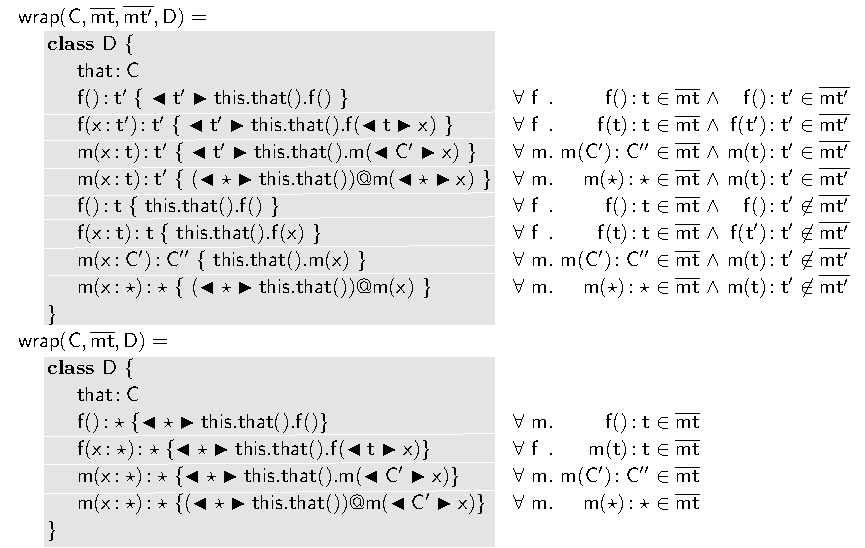
\includegraphics[width=.9\textwidth]{figures/wrapDefinition}
% TODO: untyped(mt)
% \hrulefill
% %%%%%%%%%%%%%%%%%%%%%%%%%% WRAP %%%%%%%%%%%%%%%%%%%%%%%%%%%%%%%%%%%%%%%%%%%%%%%
%   \caption{Wrapper class generation.}\label{wrap}
% \end{figure}

% \clearpage

\normalsize

\section{Generative Monotone Casts}

\subsection{Retype function}\label{retype}

Formally, the \xt{retype} function takes a list of object
addresses \b\a and a list of types to ascribe to them \b\t, and updates the
heap \s and class table \K. 

\begin{mathpar}
\IRule{CRM1}{
  \htype \a\S\s\K = \C~\Kp\\
  \tmeet\C\t\cdot\Kp = \D\,\Kpp\\ 
  \C\not\EQ\D  \\
  \ftypes \a\D \s\Kpp = \b\ap~\b\tp \\
  \Sp = \Map\S{\Bind\a\D } \\
  \retype{\b\ap}{\b\tp}\Sp\s\K = \Spp\,\K'''
}{
  \retype \a\t\S\s\K = \Spp\,\K'''
}

\IRule{CRM2}{
  \htype \a\S\s\K = \tp\,\Kp\\
  \tmeet\tp\t\cdot\Kp = \tpp\,\Kp \\
  \tp\EQ\tpp \\
}{
  \retype \a\t\S\s\K = \S~\Kpp
}

\IRule{CRM3}{
  \retype\a\t\S\s\K = \Sp\,\Kp\\
  \retype{\b\a}{\b\t}\Sp\s\Kp = \Spp\,\Kpp
}{
  \retype {\a\,\b\a}{\t\,\b\t}\S\s\K = \Spp\,\Kpp
}
\end{mathpar}

\subsection{Spec function}\label{mono:spec}

Formally, the \xt{spec} (heap specialization) function takes a
sequence of object addresses \b\a, a heap typing \S, a heap \s
and a class table \K and returns a new heap where the objects
have been retyped. \Dom\S retrieves the list of addresses 
that have to be retyped.

\begin{mathpar}
\IRule{CMS1}{
  \E \text{ fresh}\\
  \D = \App\S\a \\
  \obj\C{\ap} = \App\s\a \\
  \obj\Cp{\b\app} = \App\s\ap \\
  \classoff\Cp\Kpp = \b\mt \\
  \classoff\D\Kpp = \b\mtp \\  
  \names{\b\mtp} \subseteq \names{\b\mt}\\
  \Kp = \K~\classgen{\Cp,\b\mt,\b\mtp,\E,\K} \\
  \sp = \Map\s{\Bind\a{\E\{\ap\}}}
}{
  \spec \a\S\s\K = \sp~\Kp
}

\IRule{CMS2}{
  \spec \a\S\s\K = \sp\\
  \spec {\b\a}\S\sp\K =\spp
}{
   \spec {\a\,\b\a}\S\s\K = \spp
}
\end{mathpar}

\subsection{Meet function}\label{monmeet}

The \texttt{mmeet} function is used by the \texttt{tmeet} functions to
perform the meet over the typing of each method within a class definition.
The \texttt{mmeet} function also takes four arguments, the method
signatures of the original class $\b\mt$, the method signatures of the cast
class $\b\mtp$, the environment $\P$, a class table $\K$, and outputs method
types $\b\mtpp$ and a class table $\Kp$. \\

% \hrulefill

\opdef{
  $\mmeet{\b\mt}{\b\mtp}\P\K = \b\mtpp\,\Kp$
}{
}
\begin{mathpar}
\IRule{MM1}{
}{
  \mmeet{\b\mt}{\cdot}\P\K =\b{\mt} ~\K
}

\IRule{MM2}{
}{
  \mmeet{\cdot}{\b\mt}\P\K =\b{\mt} ~\K
}

\IRule{MM3}{ 
  \Mtype\f{}{\t} = \mt \\
  \Mtype\f{}{\tp} \in \b{\mtp} \\
  \tmeet{\t}{\tp}\P\K = \tpp~\Kp \\
  \Mtype\f{}{\tpp} = \mtpp
}{ 
   \mmeet{\mt}{\b{\mtp}}\P\K = \mtpp\,\Kp
}

\IRule{MM4}{ 
  \Mtype\f{\t}{\t} = \mt \\
  \Mtype\f{\tp}{\tp} \in \b{\mtp} \\
  \tmeet{\t}{\tp}\P\K = \tpp~\Kp \\
  \Mtype\f{\tpp}{\tpp} = \mtpp
}{ 
   \mmeet{\mt}{\b{\mtp}}\P\K = \mtpp\,\Kp
}


\IRule{MM5}{ 
  \Mtype\m{\t_1}{\t_2} = \mt \\
  \Mtype\m{\t_3}{\t_4} \in \b{\mtp} \\
  \tmeet{\t_3}{\t_1}\P\K = \t_5~\Kp \\
  \tmeet{\t_2}{\t_4}\P\Kp = {\t_6}~{\Kpp} \\
  \Mtype\n{\t_5}{\t_6} = \mtpp
}{ 
   \mmeet{\mt}{\b{\mtp}}\P\K = \mtpp\,\Kpp 
}

\IRule{MM6}{
  \mmeet{\mt}{\b{\mt_2}}\P\K = \mt_3~\Kp\\
  \mmeet{\b{\mt_1}}{\b{\mt_2}}\P\Kp = \b{\mt_4}~\Kpp
}{
  \mmeet{\mt~\b{\mt_1}}{\b{\mt_2}}\P\K =\mt_3\b{\mt_4} ~\Kpp
}
\end{mathpar}
\\

\subsection{Monotonic dynamic expression translation}\label{montrans}


\begin{mathpar}
\IRule{MREW1}{ }{ \rtranstz{\b{\mt}}{\b{\mtp}}\x\x }
\\
\IRule[width=25em]{MREW2}{ 
  \Mtype\n{\b{\t_1}}{\tp_1} \in \b{\mt} \\ 
  \Mtype\n{\b{\t_2}}{\tp_2} \in \b{\mtp} \\ 
  \n = \f \vee \t_2 \neq \any  \\ 
  \b{\rtranstz{\b{\mt}}{\b{\mtp}}{\e}{\ep}}
}{
  \rtranstz{\b{\mt}}{\b{\mtp}}{\Call{\this}\n{\b\e}}{\MonCast{\tp_1}{\Call{\this}\n{\b{\MonCast{\t_2}{\ep}}}}}
}
\\

\IRule[width=20em]{MREW3}{ 
  \Mtype\n{\b{\t_1}}{\tp_1} \in \b{\mt} \\ 
  \Mtype\n{\b{\t_2}}{\tp_2} \not\in \b{\mtp} \\ 
  \b{\rtranstz{\b{\mt}}{\b{\mtp}}{\e}{\ep}}
}{
  \rtranstz{\b{\mt}}{\b{\mtp}}{\Call{\this}\n{\b\e}}{{\Call{\this}\n{\b{{\ep}}}}}
}

\IRule[width=20em]{MREW4}{ 
  \e_1 \neq \this \\ \rtranstz{\b{\mt}}{\b{\mtp}}{\e_1}{\e_2} \\ 
  \b{\rtranstz{\b{\mt}}{\b{\mtp}}{\ep_1}{\ep_2}}
}{
  \rtranstz{\b{\mt}}{\b{\mtp}}{\Call{\e_1}\n{\b{\ep_1}}}{\Call{\e_2}\n{\b{\ep_2}}}
}

\IRule{MREW5}{ 
  \rtranstz{\b{\mt}}{\b{\mtp}}{\e_1}{\e_2} \\ 	
  \rtranstz{\b{\mt}}{\b{\mtp}}{\ep_1}{\ep_2}
}{
  \rtranstz{\b{\mt}}{\b{\mtp}}{\DynCall{\e_1}\m{\ep_1}}{\DynCall{\e_2}\m{\ep_2}}
}

\IRule{MREW6}{
  \b{\rtranstz{\b{\mt}}{\b{\mtp}}{\e}{\ep}} 
}{
  \rtranstz{\b\mt}{\b\mtp}{\New\C{\b\e}}{\New\C{\b\ep}}
}
\end{mathpar}


\subsection{Monotonic class generation}\label{classgen}

\footnotesize
\[\begin{array}{l@{~}r@{}r@{~}r@{~}r@{~}rr}
\arrayrulecolor{white}
\classgen{\C, \b\md, \bmt, \bmtp, \D, \K}= \\
\SP \class~\D~\{ \\
\SPP \Fdef\that\C
\\[1mm]
\SPP \Mdef\f\x\any\any {\SubCast\any{\MonCast\tp{
      \Set{\Get\this\that}\f{\MonCast\t{\MonCast\tp\x}}}}}
&
\All f \Mtype\f\t\t\in\bmt &\wedge& \Mtype\f\tp\tp\in\bmtp
\\[1mm]\hline
\SPP \Mdefz\f\any{\SubCast\any{\MonCast\tp{\Get{\Get\this\that}\f}}}
&
 \All f \Mtype\f{}\t \in \bmt &\wedge& \Mtype\f{}\tp \in \bmtp
\\[1mm]\hline
\SPP \Mdef\m\x\any\any {~\SubCast\any{\MonCast{\tp[2]}{{[{(\MonCast{\t[1]}\x)}/\x]\ep}}}~}
&     \All \m \Mdef\m\x{\t[1]}{\tp[1]}\e\in\b\md &\wedge& \Mtype\m{\t[2]}{\tp[2]}\in\bmtp \\
&&\wedge&\multicolumn{3}{l}{\rtranstz{\bmt}\bmtp{[{(\MonCast\t\x)}/\x]\e}{\ep}}
\\[1mm]\hline
\SPP \Mdef\m\x{\t[2]}{\tp[2]} {\MonCast{\tp[2]}{[{(\MonCast{\t[1]}\x)}/\x]\ep}~}
&     \All \m \Mdef\m\x{\t[1]}{\tp[1]}\e\in\b\md &\wedge& \Mtype\m{\t[2]}{\tp[2]}\in\bmtp \\
&&\wedge&\multicolumn{3}{l}{\rtranstz{\bmt}\bmtp{\e}{\ep}} \\
&&\wedge&\multicolumn{3}{l}{\statictype{\t[2]}{\K}{\cdot}}
\\[1mm]\hline
\SP\}
\end{array}
\]
\normalsize





\subsection{Monotonic equivalent type generation}\label{typegen}

\footnotesize
\[\begin{array}{l@{~}r@{}r@{~}r@{~}r@{~}rr}
\arrayrulecolor{white}
\typegen{\bmt}{\D} = \\
\SP \class~\D~\{
\\[1mm]
\SPP \Mdef\m\x\t\tp {{\MonCast\tp{\x}}} 
&
\All m \Mtype\m\t\tp\in\bmt
\\[1mm]\hline
\SPP \Mdef\f\x\t\t {\x}
&
\All f \Mtype\f\t\t\in\bmt
\\[1mm]\hline
\SPP \Mdefz\f\t{{\MonCast\t{\New\D{}}}}
&
 \All f \Mtype\f{}\t \in \bmt
\\[1mm]
\SP\}
\end{array}
\]
\normalsize




\subsection{Htype function}

The function \htype\a\S\s\K
returns the class of the object at address \a.  \htype\a\S\s\K is \C if \C =
\App\S\a or if $\a\not\in\S$ and \obj\C{\b\a}=\App\s\a.

\begin{mathpar}
\IRule{HT1}{
  \a \not\in \text{addr}(\S) \\
  \enfortype\C\cdot\K = \D\,\W\,\Kp
}{
  \htype\a\S{\sigma[\a \mapsto \C\{\ap\}]}\K = \D~\Kp
}

\IRule{HT2}{
  \S(\a) = \t
}{
  \htype{\a}{\S}{\sigma}\K = \t~\K
}
\end{mathpar}

\subsection{Lifting function}

% \hrulefill
\begin{align*}
\W &::= \cdot \B \Map\W{\Bind\C\D}
\end{align*}
\begin{mathpar}
\IRule{ENT1}{ 
  \Class\C{\hspace{-0.3em}}{\Fdef\that\Cp ~ \b\md} \in \K \\ 
  \C \notin \text{dom}(\W) \\
  \D\text{ fresh} \\
  \Wp = \W\,\Bind\C\D \\
  \Kp = \K\,\Class\D{\hspace{-0.3em}}{\Fdef\that\Cp ~ \enformt{\b{\md}}{\Wp}{\K}} \\ 
}{
  \enfortype{\C}{\W}{\K} = \D\,\Wp\,\Kp
}

\IRule{ENT2}{ 
  \W(\C) = \D \\
}{
  \enfortype{\C}{\W}{\K} = \D\,\W\,\K
}

\IRule{ENT3}{ 
}{
  \enfortype{\any}{\W}{\K} = \any\,\W\,\K
}
\end{mathpar}
\\

% \hrulefill

\begin{mathpar}
\IRule{ENMT1}{
  \md =  \Mdef\m\x\any\any {~\SubCast\any{\MonCast\tp{{[{(\MonCast\t\x)}/\x]\ep}}}~} \\
  \enfortype\t\W\K = \tpp\,\Wp\,\Kp \\
  \enfortype\tp\Wp\Kp = \tppp\,\Wpp\Kpp \\
  \mdpp = \Mdef\m\x\tpp\tppp {\MonCast\tppp\x} \\
  \enformt{\b\md}{\Wpp}{\Kpp} = \b\mddp \\
}{
  \enformt{\md\,\b\md}{\W}{\K} = \mdpp\,\b\mddp
}

\IRule{ENMT2}{
  \md = \Mdef\m\x\t\tp {\ep~}\\ 
  \enfortype\t\W\K = \tpp\,\Wp\,\Kp \\
  \enfortype\tp\Wp\Kp = \tppp\,\Wpp\Kpp \\  
  \mdpp =\Mdef\m\x\tpp\tppp {\MonCast\tppp\x}\\
  \enformt{\b\md}{\Wpp}{\Kpp} = \b\mddp \\
}{
  \enformt{\md\,\b\md}{\W}{\K} = \mdpp\,\b\mddp
}

\IRule{ENFS}{
  \md = \Mdef\f\x\any\any {\SubCast\any{\MonCast\tp{\Set{\Get\this\that}\f{\MonCast\t{\MonCast\tp\x}}}}} \\ 
  \enfortype\t\W\K = \tpp\,\Wp\,\Kp \\
  \enfortype\tp\Wp\Kp = \tppp\,\Wpp\Kpp \\   
  \mdpp = \Mdef\f\x\tpp\tppp {\MonCast\tppp\x} \\
  \enformt{\b\md}{\Wpp}{\Kpp} = \b\mddp \\
}{
  \enformt{\md\,\b\md}{\W}{\K} = \mdpp\,\b\mddp
}

\IRule{ENFG}{
  \md =  \Mdefz\f\any{\SubCast\any{\MonCast\t{\Get{\Get\this\that}\f}}} \\ 
  \enfortype\t\W\K = \tp\,\Wp\,\Kp \\
  \mdpp = \Mdefz\f\tp {\MonCast\tp{\Get{\Get\this\that}\f}} \\
  \enformt{\b\md}{\Wp}{\Kp} = \b\mddp \\
}{
  \enformt{\md\,\b\md}{\W}{\K} = \mdpp\,\b\mddp
}

\IRule{ENE}{
}{
  \enformt{\cdot}{\W}{\K} = \cdot
}
\end{mathpar}

\subsection{Static function}

\opdef{
  $\statictype\D\K{\b\C} = \texttt{Bool}$
}{
}

\begin{mathpar}
\IRule{ST1}{ 
}{ 
  \statictype\any\K{\b\C} = \texttt{False} 
}

\IRule{ST2}{ 
 \D \in {\b\C}
}{ 
  \statictype\D\K{\b\C} = \texttt{True} 
}

\IRule{ST3}{
  \D ~\text{empty}
}{ 
  \statictype\D\K{\b\C} = \texttt{True} 
}

\IRule{ST4}{
 \Class \C {\b{\Ftype\f\t}}{\b\md} \in \K \\
 \sign{\b\md} = \b{\Mtype\m\tp\tpp} \\ 
 \b\Cp = \b\C, \D
}{ 
  \statictype\D\K{\b\C} = \statictype{\b\t}\K{\b\Cp} \cap \statictype{\b\tp}\K{\b\Cp} \cap \statictype{\b\tpp}\K{\b\Cp}
}
\end{mathpar}
\\

\subsection{Wftype function}

\wftype{\b\f}\C\K denotes the function that looks up the type of a particular set of fields in \C.

\begin{equation*}
\wftype{\b\f}\C\K = \b\t ~~\mathit{if}~~ \begin{cases}

 \Class \C {\b{\Ftype\fp\tp}}{\b\md} \in \K\\
 \b\t = \{ \b\t \subseteq \b\tp ~|~ \forall~ \f \in \b\f ~.~ \f \in \names{\b{\Ftype\fp\tp}} \} \\
 
\end{cases}
\end{equation*}

\subsection{Mtype function}

The \texttt{mtypes} function takes a class name $\C$ and the class table
$\K$, and outputs a list of typing signatures $\b\mt$ for every method in
class $\C$, which includes the implicit getter and setter methods for every
field in the definition of class $\C$.  (\textbf{Note}: An user cannot
define a getter or setter method for any field that already exists in the
class. Similarly, a field cannot be declared in a class that already has a
getter or setter method for that field. This is enforced by the
\texttt{overloading} function in class well-formedness.)

\begin{equation*}
\classoff\C\K = \b\mt ~~\mathit{if}~~ \begin{cases}

 \Class \C {\b{\Ftype\f\t}}{\b\md} \in \K\\
 \b\mt = \sign{\b\md} \oplus \forall ~\Ftype\f\t \in \b{\Ftype\f\t} ~|~ \f \notin \names{\b\md} ~\wedge~ \f\neq\that ~.~ \typez{\Ftype\f\t}

\end{cases}
\end{equation*}

\subsection{getmds function}

$\getmds\C\K$ denotes the function that returns the method definitions inside the class \C.

\begin{equation*}
\getmds\C\K = \b\md ~~\mathit{if}~~ \Class\C{\b{\fd}}{\b\md} \in \K
\end{equation*}

\subsection{Ftype function}

The function \ftypes\a\C\s\K returns the old references and the new types
for them according to the new wrapper \C.

\begin{mathpar}
\IRule{FT1}{
 \App\s\a=\obj\D{\ap} \\ % we know that a refers to a wrapper with a that field of the wrapped object
  \App\s\ap =\obj\E{\b\app}  \\ % getting the fields out of ap
 \Class \E {\b{\Fdef\f\t}}{\b\md} \in\K \\
 \wftype{\b\f}\C\K =\b\tp
}{
  \ftypes \a\C\s\K = \b\app~\b\tp
}
\end{mathpar}


\subsection{Dynamic function}

\begin{mathpar}
\IRule{DYN1}{
 \dyn{\b\mt} = \b{\mtp} \\
}{
  \dyn{\Mtype{\m}{\t}{\t} ~\,\b\mt} = \Mtype{\m}{\any}{\any}~\,\b\mtp
}

\IRule{DYN2}{
 \dyn{\b\mt} = \b{\mtp} \\
}{
  \dyn{\Mtype{\f}{\t}{\t} ~\,\b\mt} = \Mtype{\f}{\any}{\any}~\,\b\mtp
}

\IRule{DYN3}{
 \dyn{\b\mt} = \b{\mtp} \\
}{
  \dyn{\Mtype{\f}{}{\t} ~\,\b\mt} = \Mtype{\f}{}{\any}~\,\b\mtp
}

\IRule{DYNE}{
}{
  \dyn{\cdot} = \cdot
}
\end{mathpar}

\subsection{Signature function}

\begin{mathpar}
\IRule{SGE}{
}{
  \sign{\cdot} = \cdot
}

\IRule{SG1}{
  \md = \Mdef\m\x\t\t\e \\
  \sign{\b\md} = \b\mt \\
}{
  \sign{\md\,\b\md} = \Mtype\m\t\t~~\b\mt
}

\IRule{SG2}{
  \md = \Mdef\f\x\t\t\e \\
  \sign{\b\md} = \b\mt \\
}{
  \sign{\md\,\b\md} = \Mtype\f\t\t~~\b\mt
}

\IRule{SG3}{
  \md = \Mdefz\f\t\e \\ 
  \sign{\b\md} = \b\mt \\
}{
  \sign{\md\,\b\md} = \Mtype\f{}\t~~\b\mt
}
\end{mathpar}

\subsection{Typing function}

\begin{mathpar}
\IRule{TY1}{
}{
  \typez{\Ftype\f\t} = \Mtype\f\t\t~~\Mtype\f{}\t
}
\end{mathpar}

% \section{Monotonic examples in Reticulated Python}
% 
% \begin{lstlisting}[language=python]
% class C:
% 	def m1(self,v:Int,g:Dyn)->Dyn:
% 		return 2
% 
% class D:
% 	def m1(self,v:Dyn,g:Int)->Dyn:
% 		return 2
% 
% class E:
% 	def m1(self,v:Int,g:Int)->Dyn:
% 		return 2
% 
% def castC(e:C) -> C:
% 	return e
% 
% e = E()
% c = castC(e)
% c.m1(2,2)
% \end{lstlisting}
% 
% 
% \begin{lstlisting}[language=python]
% class C:
% 	def m1(self,x:C,v:Int,g:Dyn)->Dyn:
% 		return 2
% 
% class D:
% 	def m1(self,x:D,v:Dyn,g:Int)->Dyn:
% 		return 2
% 
% class E:
% 	def m1(self,x:E,v:Int,g:Int)->Dyn:
% 		return 2
% 
% def castD(e:D) -> D:
% 	return e
% 
% c = C()
% d = castD(c)
% c.m1(c,2,2)
% \end{lstlisting}
% 
% 
% \begin{lstlisting}[language=python]
% class C:
% 	def m1(self,x:C)->Dyn:
% 		return 2
% 
% class E:
% 	def m1(self,x:E)->Int:
% 		return 2
% 
% c = C()
% c.m1(c)
% \end{lstlisting}
% 
% 
% \begin{lstlisting}[language=python]
% class C:
% 	def m1(self,x:C)->Dyn:
% 		return 2
% 
% class E:
% 	def m1(self,x:E)->Int:
% 		return 2
% 
% def castE(e:E) -> E:
% 	return e
% 
% c = C()
% e = castE(c)
% c.m1(C())
% \end{lstlisting}


%% Example -- please check

%% class A {
%%   fa : B
%%   ma(x : A): B { fa.mb(a) }
%% }
%% class B {
%%   fb : any
%%   mb(x:A):B { this }
%% }
%% class C {}

%% class Ap {
%%   fa : Bp
%%   ma(x : Ap): Bp {...}
%% }
%% class Bp {
%%   fb: C 
%%   ma(x : Ap): Bp {...}
%% }

%% a = new A(new B(new C()))
%% ap = <| Ap |> a

%% class WA {
%%   that : A
%%   fa() : B { that.fa() }
%%   fa(x:B):B { that.fa(x) }
%%   ma(x:B):B { that.ma(x) }
%% }
%% class WB {
%%   that : any
%%   fb() : any { that.fb() }
%%   fb(x:any):any { that.fb(x) }
%%   mb(x:B):B { that.mb(x) }
%% }
%% class WBp {
%%   that : A
%%   ...

%% Example -- please check

%%class A {
%%  m(x:*):* { x }  
%%}
%% a = new A()
%% a.m(new A()) -- works fine
%%class B {
%%  m(x:B):B { x }  
%%}
%% b = <|B|> a
%% b.m(new B()) -- works
%% a.m(new A()) -- fails

% translated version

%%class wA {
%%  that : A
%%  m(x:*):* { this.that().m(x) }
%%}
%%a = new wA(new A())
%%(<*>a)@(<*>new wA(new A()))
%%class AmB {
%%  m(x:B):B{ ... }
%%}
%%class AwAmB {
%%  that : A
%%  m(x:*):* { <|*|><|B|>(<|*|>this.that())@m(<|*|><|B|>x) }
%%  m(x:B):B { <|B|>(<|*|>this.that())@m(<|*|>x)}  
%%}
%% b = <|B|> a -- b and a instance of AwAmB
%% b.m(new B()) -- works
%% a.m(new A()) -- fails

% example 2

%% class T { }
%% class A { f : * }
%% class B { f : A }
%% class C { f : B }
%% a1 = new A(new T())
%% a2 = new A(a1)
%% a3 = new A(a2)
%% b = <|B|> a3
%% c = <|C|> a3

% translated

%% class WA { that : A f():* { <|*|><|*|> this.that().f() } f(x:*):* { <|*|><|*|> this.that().f(<|*|><|*|>s x)} }
%% class WAmB { that:A f():* { <|*|><|A|>this.that().f() } f(x:*):* {<|*|><|A|> this.that().f(<|*|><|A|> x) } }
%% class WAmBmC { that:A f():* {<|*|> <|B|> this.that().f() } f(x:*):* { <|*|> <|B|> this.that().f(<|*|><|B|> x)} }
%% a1 = new WA(new A(new WT(new T())))
%% a2 = new WA(new A(a1))
%% a3 = new WA(new A(a2))
%% b = <|B|> a3 -- s(b) : WAmB
%% a3.f(new T()) -- boom
%% a2.f(new T()) -- ok
%% c = <|C|> b -- s(b) : WAmBmC, s(a2) : WAmB
%% a3.f(new T()) -- boom
%% a3.f(new WA(new A(new T))) -- boom
%% a2.f(new T()) -- boom

%% class A {
%%   fa : B
%%   ma(x : A): B { fa.mb(a) }
%% }
%% class B {
%%   fb : any
%%   mb(x:A):B { this }
%% }
%% class C {}

%% class Ap {
%%   fa : Bp
%%   ma(x : Ap): Bp {...}
%% }
%% class Bp {
%%   fb: C 
%%   ma(x : Ap): Bp {...}
%% }

%% a = new A(new B(new C()))
%% ap = <| Ap |> a

%% class WA {
%%   that : A
%%   fa() : B { that.fa() }
%%   fa(x:B):B { that.fa(x) }
%%   ma(x:B):B { that.ma(x) }
%% }
%% class WB {
%%   that : any
%%   fb() : any { that.fb() }
%%   fb(x:any):any { that.fb(x) }
%%   mb(x:B):B { that.mb(x) }
%% }
%% class WBp {
%%   that : A
%%   ...


% \section{Proofs of Related Theorems}
% \subsection{Accessory Lemmas}
% 
% \paragraph{Evaluation Extends Class Tables}
% 
% If $\Reduce \K\e\s \Kp\ep\sp$ then $\Kp = \K~\Kpp$ for some $\Kpp$.
% 
% \paragraph{Weakening of Subtyping}
% 
% If $\StrSub\cdot\K\t\tp$ then $\StrSub\cdot{\K~\Kp}\t\tp$.
% 
% \paragraph{Correctness of \classoff{\C}{\K}}
% 
% If $\Mtype\n{\b\t}\tp \in \classoff{\C}{\K}$, $\EnvType\cdot\s\K\e\C$ and (if applicable) $\EnvType\cdot\s\K\ep\t$, then $\Reduce \K{\Call\e\n{\b\ep}}\s \K\epp\s$ where $\EnvType\cdot\s\K\epp\tp$
% 
% \subsection{Soundness of \kafka Typing}
% 
% Given that $\WFp\K\e\s$ and $\EnvType\cdot\s\K\e\t$, then either there is some $\ep$ such that $\Reduce \K\e\s \Kp\ep\sp$ and $\WFp\Kp\ep\sp$ and $\EnvType\cdot\sp\Kp\ep\t$ hold, or $\e$ is of one of the following forms:
% \begin{itemize} 
% \item $\a$
% \item $\DynCall\ep\m{\epp}$
% \item $\SubCast\tp\ep$
% \item $\ShaCast\tp\ep$
% \item $\BehCast\tp\ep$
% \item $\MonCast\tp\ep $
% \end{itemize}
% We proceed with rule induction on the judgement used to conclude $\EnvType\Env\s\K\e\t$. Note that we refer to rule preconditions from left to right.
% \begin{itemize}
%   \item W1
% 
%         Not applicable, since $\Gamma = \cdot$ and therefore contains no variables.
%   \item W2
% 
%         We apply the IH to the first precondition. If we get stuck in the IH, then the entire expression gets stuck or terminates, trivially. Therefore, the interesting case is when $\Reduce \K\e\s \Kp\ep\sp$, $\WFp\Kp\ep\sp$ and $\EnvType\cdot\sp\Kp\ep\tp$. By 
%   \item W3, W4, W5
%   \item W6
%   \item W7
%   \item W8
%   \item W9
%   \item W10
%   \item W11
%   \item W12
% \end{itemize}
% 
% \subsection{Type Correctness of Translation}


\end{document}

%######## ##    ## ########      #######  ########    ########   #######   ######  ##     ## ##     ## ######## ##    ## ######## 
%##       ###   ## ##     ##    ##     ## ##          ##     ## ##     ## ##    ## ##     ## ###   ### ##       ###   ##    ##    
%##       ####  ## ##     ##    ##     ## ##          ##     ## ##     ## ##       ##     ## #### #### ##       ####  ##    ##    
%######   ## ## ## ##     ##    ##     ## ######      ##     ## ##     ## ##       ##     ## ## ### ## ######   ## ## ##    ##    
%##       ##  #### ##     ##    ##     ## ##          ##     ## ##     ## ##       ##     ## ##     ## ##       ##  ####    ##    
%##       ##   ### ##     ##    ##     ## ##          ##     ## ##     ## ##    ## ##     ## ##     ## ##       ##   ###    ##    
%######## ##    ## ########      #######  ##          ########   #######   ######   #######  ##     ## ######## ##    ##    ##    




\subsection{others}

%TODO Fix ME \mtype\m\C\K = \convert{\methz\m\C\K} 

\hrulefill

\opdef{\classoff\C\K}{Auxiliary function: Type definition}

\begin{equation*}
\classoff\C\K = \EMxt{MT} ~~s.t.~~ \begin{cases}

 \K(\C) = \Class \C {\b{\Ftype\f\t}}{\b\md} \\
 \EMxt{MT} = \{\convert{\b\md} \oplus \forall ~\Ftype\fp\tp \in \b{\Ftype\f\t} ~|~ \fp \notin \b{\names{\md}} ~.~ \convertFD{\Ftype\fp\tp}\}

\end{cases}
\end{equation*}

\hrulefill


\opdef{\classoffs\a\s\K}{Auxiliary function: Type definition}

\begin{equation*}
\classoffs\a\s\K = \EMxt{MT} ~~s.t.~~ \begin{cases}

 \s(\a) = \obj\C{\b\a} \\
 \K(\C) = \Class \C {\b{\Ftype\f\t}}{\b\md} \\
 \EMxt{MT} = \{\convert{\b\md} \oplus \forall ~\Ftype\fp\tp \in \b{\Ftype\f\t} ~|~ \fp \notin \b{\names{\md}} ~.~ \convertFD{\Ftype\fp\tp}\}

\end{cases}
\end{equation*}

\hrulefill

\opdef{\ftype\f\C\K}{Auxiliary function: Field type lookup}

\begin{equation*}
\ftype\f\C\K = \t ~~s.t.~~ \begin{cases}

 \K(\C) = \Class \C {\ldots ~ \Ftype\f\t ~ \ldots}{\b\md}
\end{cases}
\end{equation*}

\hrulefill

\opdef{\field\C\K}{Auxiliary function: Field definition}

\begin{equation*}
\field\C\K = \b{\Ftype\f\t} ~~s.t.~~ \begin{cases}

 \K(\C) = \Class \C {\b{\Ftype\f\t}}{\b\md}
\end{cases}
\end{equation*}




This common core is focused on the basics of object functionality, with a
simple example being a \xt{Point} class.\footnote{For our examples we use
  integers and common arithmetic operations even if they are not in core
  calculus.}

%%% FIXME: formatting
\begin{verbatim}
class Point {
  x : Int
  y : Int
  addx( v : Int ) : Int {
       this.x!( this.x() + v )
  }
  addy( v : Int ) : Int {
       this.y!( this.y() + v )
  }
}
\end{verbatim}

The type system ensures that, if \xt{pt} is declared to be of type
\xt{Point}, an operation such as \xt{pt.addx(42)} will not get stuck.  As
this small language requires all variables to be initialized, there checking
for \xt{null} is not needed as it likely would in a full fledged language.

The language also supports a single unconstrained type, denote \any (pronounced
dyn), thus one could write the following method

%%% FIXME: formatting
\begin{verbatim}
  mkPt( u : * ) : Point {
      new Point( u.x() 
                 (<Point> u).y() )
  }
\end{verbatim}

This method will accept an instance of any class and will return a new
\xt{Point}. At run-time, the code will get stuck if the dynamic cast
\xt{\Cast{\xt{Point}}{\xt{u}}} fails. If \x is a declared of type \any, an
expression such as \xt{u.x()} will fail if the object bound to \xt{u} does
not have a getter \xt{x()}.


%%%%%%%%%%%%%%%%%%%%%% DYNAMIC SEMANTICS %%%%%%%%%%%%%%%%%%%%%%%%%%%%%%%%%%%%%%

The dynamic semantics evaluates expression extended with object references,
denoted \a, and errors, denoted \err, together with a heap \s mapping
references to object values. Object values contain all fields, methods, a
type, and a class; they are denoted \obj\C{\b\a}. The class is used for
locating methods and the type is used for type casts. The need for keeping
them separate will become clear later.

The semantics uses evaluation context \E[\e], meaning that $\e$ is in the
hole of $\E$. Selecting an object from the heap is written \Sel\s\a, while a
heap is extended with a new object by \Map{\s}{\Bind{\a}{\obj\C{\dots}}}.

For an object reference \a, such that \EM{\Sel\s\a=\obj\C\dots}, we have 
\classofis{\Sel\s\a}\C and \typeofis\s\a\t.

We use the notation \Mdef\m\x\t\t \in\C to select a method in a class
definition and \Fdef\f\t\a\in\obj\C\dots to express the selection of a
field. Lastly a field of an object can be update with the notation
\Update{\obj\C\dots}\f\a.

\subsection{Core Type System}

As a basis for our gradual type system, we will use a simple static
type system, ensuring that the program will not get stuck, but while
simultaneously is entirely up-front and not gradual, shown in
figure~\ref{fig:basetyp}.

This basic type system is typical of calculi that support objects, notably
including subtyping. Subtyping in our system is defined in
figure~\ref{fig:sub}, which defines a simple structual subtyping system with
names (to provide for recursive types) as well as the Amber rule to support
recursive types. Notably, however, because there are no valid operations on
$\any$ other than casting, this type system cannot be called a
\emph{gradual} type system, as a gradual type system should allow $\any$
typed-terms to coexist with fully typed ones.

Soundness for this base system is typical. We combine the progress and
preservation lemmas to come up with an aggregate small step soundness
theorem, which we then extend with the typical cast failure carve-out to
enable casts to fail without the program getting stuck.

\begin{thm}
If $\EnvType\Es\e\t$, then one of the following holds:
\begin{itemize}
\item $\e \rightarrow \e'$ and $\EnvType\Es{\e'}\t$
\item $\e \rightarrow \xt{v}$ and $\EnvType\Es{\xt{v}}\t$
\item $\e$ is $\Cast{\t}{\e'}$ and $\e \rightarrow \err$
\end{itemize}
\end{thm}

\begin{figure}
%!TEX root = ../ss.tex
\opdef{\EnvType{\Es}\e\t}{\e has type \t in environment \E against heap \s}
\begin{mathpar}
\IRule{W1}{
    \HasType{\E}\x\t
 }{
   \EnvType{\Es}\x\t
}

\IRule{W2}{
   \EnvType{\Es}\e{\tp 1} \\ {\tp 1} \Sub {\t}
 }{
   \EnvType{\Es}\e\t 
}   

\IRule{W4}{
   \EnvType{\Es}\e{\t} \\ \Mtype\m{\b{\tp2}}{\tp3}\inc \t  \\  \b{\EnvType{\Es}{\ep1}{\tp 2}}
}{
    \EnvType{\Es}{\Call\e\m{\b{\ep1}}}{\tp3}
}    

\IRule{W5}{
  \b{\EnvType{\Es}\e\t} \\ 
  \Class \C {\b{\Ftype\f\t}} {\b{\md}}
}{
  \EnvType{\Es}{\New\C{\b\e}}\C
}

\IRule{W6}{
  \EnvType{\Es}\e{\tp1}
}{
   \EnvType{\Es}{\Cast\t\e}\t
}

\IRule{W7}{
  \EnvType{\Es}{\ep1}{\tp1} \\
  \f : \t \in \tp1 \\
}{
  \EnvType{\Es}{\Get\e\f}{\t}
}

\IRule{W8}{
  \EnvType{\Es}{\ep1}{\tp1} \\
  \f : \t \in \tp1 \\
  \EnvType{\Es}{\ep2}{\t}
}{
  \EnvType{\Es}{\Set{\ep1}\f{\ep2}}\t
}

\IRule{W9}{
  \s(\ap1) = \Obj{\b{\f=\ap2}}{\C} \\ \b{\f:{\tp2} \in \C} \\ \b{\EnvType{\Es}{\ap2}{\tp2}} \\ 
}{
  \EnvType{\Es}{\ap1}{\C}
}
\end{mathpar}
\caption{Typing rules for the base langauge}
\label{fig:basetyp}
\end{figure}


\section{Gradual Typing}
In order to extend the core calculus to enable programmers to write
gradually typed code without having to insert a great number of casts
manually, we use gradual type systems to add casts where required,
presenting a unified gradual semantics to the programmer while relying on
the core system for soundness.

Our characterization of gradual typing is \emph{gradual typing by translation},
using an approach similar to that of~\cite{Bierman10}, adding gradual
types to the underlying fully typed language. In this vein,
we define our gradual typing extensions as \emph{cast insertion} phases.

\subsection{Cast Insertion}

The user-facing component of a gradual typing system is its type checker,
or the surface type system, which is then complemented by a type-driven
cast insertion mechanism ``behind the scenes''. In our approach, these two
steps are combined into a cast insertion system.

Cast insertion is fundamentally \emph{type driven}. In our type system, it is
required to have a cast whenever a type needs to be altered, and therefore in
inserting casts we need to know every site where one type is required to be another.
Our system handles this through an \emph{bidirectional cast insertion} system,
introduced by~\cite{lti-pierce}

Our choice comes from an observation about the nature of traditional
bottom-up type systems. The fundamental building block is judgements of the
form $\E \vdash \e : \t$, which means that $\e$ inherently has type
$\t$. For example, a type mismatch would look like trying to conclude a
judgement $\E \vdash \e : \any$ when only $\E \vdash \e : \xt{int}$ holds.

Other systems have solved this problem through the introduction of
nondeterministic rules such as subsumption, but nondeterminism in cast
insertion creates problems where a single program can be typed in multiple
different ways (EXAMPLE).

To solve this problem, we use the aforementioned bidirectional cast
insertion mechanism. Ina bidirectional system, we have two judgements:

\begin{itemize}
\item The \emph{analytic} judgement $\E \vdash \e \Rightarrow \t$, which says that
$\e$ inherently has type $\t$ against environment $\E$, equivalently to the
traditional bottom-up type system.
\item The \emph{synthetic} judgement $\E \vdash \e \Leftarrow \t$, which implies that
$\e$ can potentially have type $\t$ against environment $\E$.
\end{itemize}

For example, consider the function call $\Call{\ep1}{\m}{\ep2}$. A
bidirectional type system will begin with seeing what type $\ep1$ has, with
the judgment $\E \vdash \ep1 \Rightarrow \t$.  From this, the bidirectional
type system will check what type the method $\m$ has in $\t$, here denoted
$\Mtype\m{\tp1}{\tp2} \in \t$, then ensure that the arguments make sense
with that type.

In a bottom-up type system, we would write $\E \vdash \ep2 : \tp1$, but, as
commonly noted with subsumption, this can require the introduction of a
nonalgorithmic rule to conclude this final judgment. Instead, in a
bidirectional type system, we can simply ensure that the type of $\ep2$ is
consistent with $\tp1$ through the judgment $\E \vdash \ep2 \Leftarrow
\tp2$.

Finally, we will be able to conclude that $\E \vdash \Call{\ep1}{\m}{\ep2}
\Rightarrow \tp2$. This is a synthetic judgement as $\tp2$ is the type that
the expression can be known to have in the absence of any external
information.

To support cast insertion, we extend these basic type checking judgements
with an output term, of the form $\GenCast{\E}{\ep1}{\ep2}{\t}$ for the
synthetic case and $\AnaCast{\E}{\ep1}{\ep2}{\t}$ for the analytic, case,
where the former translates $\ep1$ to $\ep2$ producting type $\t$, and the
latter translates the same ensuring type $\t$.

An important note in the construction of our bidirectional type system is
that our handling of the key case, function application, is less specific
than it could be, as we ignore the analytic case. Other works in this area,
including~\cite{bidir-typing} use a third bidirectional judgment to handle
function application, largely to handle the analytic case. If we are trying
to typecheck a function call against some known type, then we can infer a
type for the receiver by using synthetic type checking on the arguments.
However, in our context, detailed handling of this case is not required, as
our type inference does not need to be as precise as it does for Dunfield
and Krishnaswami's type inference.

\subsection{Class Translation}

A key component of many gradual type systems is enabling checks for every
field access or modification, ensuring type invariants about the heap. To
enable these checks, we cannot expose ``raw'' field access and modification
in our calculus, as otherwise these checks could be easily bypassed.

As a result, we expose no typing judgment for field manipulation, and
instead auto-generate getter and setter methods in a phase we call
\emph{class translation}, occuring at the same time as cast insertion.

Another issue solved by class translation is that raised by calling a method
on a dynamic receiver type.  Consider the invocation $\Call{\e}{\m}{\e'}$
where $\EnvType{\Es}{\e}{\any}$ and $\EnvType{\Es}{\e'}{\any}$.  Now,
suppose that we have a method on $\e$ $\m(\x:\C)$. Using casting, we can
figure out that the method exists, and that the arity is correct, but there
is no static way to know the argument types of $\m$ statically to insert
checks.

Class translation solves this problem by creating a ``guard'' method
$\m_\xt{u}$ that will have the same arity and a related name, but only has
arguments of type $\any$. We then translate every call to a method $\m$ on
an untyped receiver to a call to a call to $\m_\xt{u}$, which then does the
approperiate type check before calling the typed method. Likewise, method reads and writes are protected by getters and setters added
during the class translation phase.

%%%%%%%%%%%%%%%%%%%%%%%% SUBTYPING %%%%%%%%%%%%%%%%%%%%%%%%%%%%%%%%%%%%%%%%

\begin{figure}
%%!TEX root = ../ss.tex
\opdef{$\tp1 \Sub \tp2$}{\tp 1 is a subtype of \tp 2}
\begin{mathpar}
\IRule{S-Ref}{ }{\t \Sub \t}

\IRule{S-Top}{ }{\t \Sub {\Type{}}}

\IRule{S-Rec}{
	\tp3 \Sub \tp1 \\
	\tp2 \Sub \tp4 \\
	\Type{\b{\mt_1} ~ \b{\mt_2}} \Sub \Type{\b{\mt_3}}
}{
   {\Type{\b{\mt_1} ~ \Mtype\m{\b{\tp1}}{\tp2} ~ \b{\mt_2} \,} } \Sub {\Type{\Mtype\m{\b{\tp3}}{\tp4} ~ \b{\mt_3} \,} } 
}
\end{mathpar}

\caption{Subtyping}
\label{fig:sub}
\end{figure}


%%%%%%%%%%%%%%%%%%%%%%%%% WELLFORMDNESS %%%%%%%%%%%%%%%%%%%%%%%%%%%%%%%%%%


\begin{figure}
%\opdef{$\GenCast\E{\ep1}{\ep 2}\t$}{\ep1 translates to \ep2 in environment \E with type $\t$}
\begin{mathpar}
\IRule{A1}{\HasType{\E}\x\t}{\GenCast\E\x\x\t}

\IRule{A2}{\GenCast\E{\ep1}{\ep2}{\C} \\ \f:\t \in \C }{\GenCast{\E}{\Get{\ep1}\f}{\Call{\ep2}\f{}}{\t}}

\IRule{A3}{\GenCast\E{\ep1}{\ep3}{\C} \\ \GenCast\E{\ep2}{\ep4}{\tp1} \\ \f:\tp2 \in \C \\ \tp1 <: \tp2 }{\GenCast{\E}{\Set{\ep1}\f{\ep2}}{\Call{\ep3}{\xt{f!}}{\ep4}}{\tp2}}

\IRule{A4}{
	\inv{\E}{\Call{\ep1}\m{\b{\ep2}}} = \ep3, \t \\
}{
	\GenCast{\E}{\Call{\e_1}\m{\b{\e_2}}}{\ep3}{\t}
}

\IRule{A5}{
  \b{\AnaCast\E{\e_1}{\e_2}\t} \\ 
  \Class \C {\b{\Ftype\f\t}} {\b{\md}}
  }{\GenCast{\E}{\New\C{\b{\e_1}}}{\New\C{\b{\e_2}}}{\C}}
\end{mathpar}
\caption{Synthetic cast insertion}
\end{figure}

%%%%%%%%%%%%%%%%%%%%%%%%% CLASS TRANSLATION %%%%%%%%%%%%%%%%%%%%%%%%%%%%%
\begin{figure}
%
\begin{mathpar}
\IRule{AASC1}{
  \GenCast{\E}{\ep1}{\ep2}{\tp2} \\
  \tp2 <: \tp1\\
}{
  \AnaCast{\E}{\ep1}{\ep2}{\tp1}
}

\IRule{AASC2}{
  \GenCast{\E}{\ep1}{\ep2}{\any} \\
}{
  \AnaCast{\E}{\ep1}{\Cast{\tp1}{\ep2}}{\tp1}
}

\IRule{AASC3}{
  \GenCast{\E}{\ep1}{\ep2}{\t} \\ \t \neq \any
}{
  \AnaCast{\E}{\ep1}{\Cast\any{\ep2}}{\any}
}
\end{mathpar}
\caption{Analytic Cast Insertion}
\end{figure}

\begin{figure}
%\begin{mathpar}
\IRule{CT1}{
 \b{ \mdp1} \equiv \b{\fcast{\md, \C}} ~~ \b{\setter\fd} ~~ \b{\getter\fd}\\  \b{\mdp2} \equiv \b{\mdp1} ~~ \b{\proxy{\mdp1}}
}{ 
  \TransClass { \Class \C {\b{\fd}} {\b{\md}} }{  \Class \C {\b{\fd}} {\b{\mdp2}} }
}

\IRule{}{
  \AnaCast{\this:\C,\;\b{\x:\tp1}}{\ep1}{\ep2}{\tp2}
}{
  \fcast{\Mdef\m\x{\tp1}{\tp2}{\ep1}, \C} \equiv \Mdef\m\x{\tp1}{\tp2}{\ep2}
}

\IRule{}{
}{
  \getter{\f:\t} \equiv \m() : \t ~ \{ \this.\f \}
}

\IRule{}{
}{
  \setter{\f:\t} \equiv \m(\x:\t) : \t ~ \{ \this.\f=\x \}
}

\IRule{}{
}{
  \proxy{\Mdef\m\x{\tp1}{\tp2}{\ep1}} \equiv \Mdef{\m_\xt{u}}\x{\any}{\any}{\Cast{\any}{\Call\this\m{\b{\Cast{\tp1}\x}}}}
}
\end{mathpar}
\caption{Class Translation}
\end{figure}
%%%%%%%%%%%%%%%%%%%%%%%%%%%%%%%%%%%%%%%%%%%%%%%%%%%%%%%%%%%%%%%%%%%%%%%%%

At this point, we have defined a not-very-useful semantics for gradual typing, 
with all of the key components but providing no additional functionality
beyond what our original statically typed core. This semantics has us
applying class translation, $\TransClass\C\C$, expression translation,
$\GenCast\E\e\e\t$ and $\AnaCast\E\e\e\t$, a dynamic semantics $\e 
\rightarrow \e$, and finally a subtyping relationship $\t <: \t$, defining the
architecture that we will follow for the remainder of the languages.


By following this structure, we can describe a semantics for our language
with the 5-tuple $(\rightharpoonup, \hookrightarrow, \rightsquigarrow, <:, \rightarrow)$.
The core would be defined as (TODO)


\subsection{Type soundness:}
Theorem 1: Type translation. If $\EnvType{\Es}\e\t$ and $\TransExp\E\e{\e'}\t$ then $\EnvType{\E ~ \cdot}{\e'}\t$.

Theorem 2: Progress. If $\EnvType{\Es}{\e}{\t}$ then $\s,\e \rightarrow \s',\e'$ for $\e'$ expression or $\e' ~ \err$.

Theorem 3: Preservation. If $\s,\e \rightarrow \s',\e'$ and $\EnvType{\Es}{\e}{\t}$ then $\EnvType{\E~\s'}{\e'}{\t}$.

For a list of classes $\bar{\c}$ such that $\b{\c ~~ WF}$ and an expression $e$ such that $\EnvnvType\cdot\e\t$ and $\b{\TransClass\c{\c'}}$, we have $\cdot~e \rightarrow^* \sigma~r$ (against $\b{\c'}$) where $r$ is either a value or $\err$.


\begin{figure}
%!TEX root = ../ss.tex
\begin{mathpar}
\IRule{UTWrap}{
	\Class\C{\b{\Mdef\m\x{\tp1}{\tp2}\e}~\b{\Mdef{\m'_u}\x{\tp1}{\tp2}\e}}
}{
	\wrapper{\C\Rightarrow\any,\xt{D}} = \Class{\xt{D}}{\xt{s} : \C}{\b{\Mdef{\m_\xt{u}}\x{\any}{\any}{\Cast{\any}{\this.\xt{s}.\m(\b{\Cast{\tp1}{\x}})}}} ~ \b{\Mdef{\m'_u}\x{\tp1}{\tp2}{\xt{s}.\m'_u(\b{x})}}}
}

\IRule{TWrap}{
	\Class\C{\b{\fd}}{\b{\md}} \\ 
}{
	\wrapper{\C\Rightarrow\{\b{\mt}\},\xt{D}} = \Class{\xt{D}}{\xt{s} : \C}{\tw{\b\md, \b\mt} ~ {\utw{\b\md, \b\mt}}}
}

\IRule{MTWrap}{
}{
  \tw{\Mdef{\m_\xt{u}}\x\any\any\e;\b{\md},\Mtype\m{\b{\tp1}}{\tp2};\b{\mt}} = \Mdef{\m}\x{\tp1}{\tp2}{\Cast{\tp2}{\this.\xt{s}.{\m_\xt{u}(\b{\Cast{\any}{\x}})}}} ~ \tw{\b{\md},\b{\mt}}
}

\IRule{MUTWrap}{
	\m \not\in\b{\mt}
}{
  \utw{\Mdef{\m_\xt{u}}\x\any\any\e;\b{\md},\b{\mt}} = \Mdef{\m_\xt{u}}\x\any\any\e ~ \utw{\b{\md},\b{\mt}}
}
\end{mathpar}
\caption{Translation for Typed Racket}
\end{figure}

Typed Racket uses a much stricter definition of where $\any$ types can go, where every class is either fully typed or fully untyped. To describe this, we alter definition 1 and 2 to


\begin{definition} A Typed Racket class table is well-formed if for every class \C  in
the class table, every method is of the form \Mdef\d\x{\tp1}{\tp2}\e where
\EnvType{\this:\C,\b{\x:\tp1}}\e{\tp2} holds in \C, and all types in \C are either $\any$ or all not $\any$
\end{definition}

Typed Racket uses wrappers to ensure that typed code type guarantees are not violated, and that untyped code follows the types that it is casted to. We generate these wrappers using the following mechanism.

\begin{definition}
Every place a type \Type{\mt} where $\mt=\Mtype\m{\b{\tp1}}{\tp2}$ flows from typed into untyped code, generate a wrapper $\Class{\C'}{~\xt{orig}:\t,\b{\md}}$ where $\md = \Mdef\m\x{\any}{\any}{\Cast{\any}{\xt{this}.\xt{orig}.\m(\b{\Cast{\tp1}x})}}$.
\end{definition}

To model Typed Racket, we then need to enforce the property that objects are wrapped at typed/untyped boundaries, and ensuring that untyped code cannot use typed code internally through casts. We do this by altering the completion process, giving us a new definition. We use the wrappers we generated using definition 4 to enforce the type guarantees


\begin{definition} A Typed Racket class table is completed if for every 
 \Class \C {\b{\fd}} {\b{\md}} in the class table: 
 \begin{itemize}
 \item for every type \Type{\b{\md}}, add a class \xt{D} such that 
 \begin{itemize}
 \item for every method $\Mtype\m{\tp1}{\tp2} \in \b{\md}$, generate a function in \xt{D} $\Mdef\m{x}{\any}{\any}{\Cast{\any}{\New{\xt{D}}{\xt{this}.\xt{orig}.\m(\New\C{\b{\Cast{\tp1}x}})}}}$
 \end{itemize}
 \item for every field \Ftype\f\t\in\C, we add to \C:
 \begin{itemize}
 \item A setter \SMdef\f\x\t\t{\Set\this\f\x} 
 \item A getter \GMdef\f\t{\Get\this\f}; 
 \end{itemize}
 \item For every method definition \Mdef\d\x\t{\tp1}\e\in\C:
 \begin{itemize}
 \item A dynamic method \Mdef{\Dyn\d}\x\any\any{\Cast\any{\Call\this\d{\b{\Cast\t\x }} }} is added to \C 
 \item We replace the body \e of \m is replaced by \ep1 where \TransClass\e{\ep1}.
 \end{itemize}
 \end{itemize}
\end{definition}

One of the issues inherent to the Strongscript approach (and is apparent in
the common core as well) is that a strict interpretation of the static type
system causes the programmer to have to write a very large number of
``obvious'' casts, breaking untyped code and seemingly-sensible typed
code. We can solve this by having the compilation process insert the types
for the programmer, which we describe using a cast insertion system.

Our cast insertion approach is based on a bidirectional type
system~\cite{}, where each expression either \emph{synthesizes}, or
inherently makes, a type, or is \emph{analyzed} against a type where the
type system checks to make sure that the expression still ``works'' under
the given type. This approach has been used for a number of other tasks,
including inferring types to select sub-languages~\cite{}, infer
types for higher rank languages~\cite{}. In our case, they allow us
to simply specify in an extensible manner where to insert casts.

Synthetic cast insertion is closer to a traditional type system, as it
produces types from terms in a similar manner. However, instead of having
non algorithmic cases where types are known (for example, in the arguments
to a typed function), the synthetic cast insertion judgment defers to the
analytic cast insertion mechanism with the known type. Importantly for us,
the basic semantics of the static type system does not change between any of
the type systems under consideration, and as a result the synthetic cases
are not changed by any of the systems.

Analytic cast insertion ensures that an expression is of a given type. We use analytic cast insertion when a type is known for an expression and we want to force that expression to be of the correct type, which we do by inserting the appropriate cast. The actual details of analytic cast insertion vary depending on the system under consideration (most notably, the monotonic semantics has a notion of consistency that differs from the other two systems).

\begin{figure}
$\t = \ldots \B {\WType{\Mtype\m\t\t}}$
\caption{Strongscript}
\end{figure}

\begin{figure}
%\begin{mathpar}
\IRule{A5}{
	\GenCast{\E}{\e_1}{\e_3}{\tp1} \\
	\Mtype{\m}{\b{\tp2}}{\tp3} \in \tp1 \\
	\b{\AnaCast{\E}{\e_2}{\e_4}{\tp2}} \\
}{
	\GenCast{\E}{\Call{\e_1}\m{\b{\e_2}}}{\Cast{\tp3}{(\Call{\e_3}{\m_u}{\b{\Cast{\any}{\e_4}}})}}{\tp3}
}
\end{mathpar}
\caption{Transient}
\end{figure}


\section{Monotonic}

%%%%%%%%%%%%%%%% Monotonic Statics

\begin{figure}[h]
%\begin{mathpar}
\IRule{CS1}{ }{{\t} \ConsSub{\t}}

\IRule{CS2}{ }{{\any} \ConsSub{\t}}

\IRule{CS3}{ }{{\t} \ConsSub{\any}}

\IRule{CS4}{ \tp 1 \Sub \tp 2 }{{\tp 1} \ConsSub{\tp 2}}

\IRule{CS5}{
    \Mtype\m{\b{\tp1}}{\tp2} \in \t\\
	\b{{\tp3} \ConsSub{\tp1}} \\
    {\tp2} \ConsSub{\tp4} \\
    {\t} \ConsSub{\Type{\b{\md}}}
}{{\t} \ConsSub{\Type{\Mtype\m{\b{\tp3}}{\tp4} ~ \b{\md}}}}
\end{mathpar}
\caption{Consistent Subtyping}
\end{figure}

The key static difference between the monotonic semantics and the other systems we have considered is the consistent subtyping relationship. Traditional subtyping can be thought of as if a value satisfies one type, then it will satisfy any supertype of that type. Consistent subtyping encapsulates both this notion and the new idea of consistency. Consistency for objects means that two types have static type information that does not conflict - e.g. $\Type{\Ftype\f\any}$ could very well be able to replace $\Type{\Ftype\f\C}$, though we are unable to tell statically. Consistency allows us to interchange these types, inserting a cast where required.

Subtype consistency combines the two properties. Subtyping lets us add and remove fields from a type, and consistency allows us to make the type we are going to more or less dynamic. Going by the above intuition, a value of type $\any$ could work with any other type and vice versa, and clearly two identical types are compatible. The most complex case is when we have two class types, both with the same method $\m$, which we resolve by ensuring that $\m$ has parameters and return types that are consistent and continuing on through the rest of the class.

Adding this to our static type system is simple. We just introduce the rule that allows types to be converted via $\stcons{}{}$. The details of how to make the dynamics work with this static addition will be covered later.

\begin{figure}[h]
%\opdef{$\meet{\tp1}{\tp2} \equiv \tp3$}{The most specific type common to $\tp1$ and $\tp2$ is $\tp3$}
\begin{mathpar}
\IRule{M1}{ }{\meet{\t}{\any} \equiv \t}

\IRule{M2}{ }{\meet{\any}{\t} \equiv \t}

\IRule{M3}{ }{\meet{\t}{\t} \equiv \t}

\IRule{M4}{
	\b{\meet{\tp3}{\tp1}  \equiv \tp5} \\
    \meet{\tp2}{\tp4} \equiv \tp6\\
    \meet{\Type{\b{\md_1}}}{\Type{\b{\md_2}}} \equiv \Type{\b{\md_3}} 
}{\meet{\Type{\Mtype\m{\b{\tp1}}{\tp2}~ \b{\md_1}}}{\Type{\Mtype\m{\b{\tp3}}{\tp4} ~ \b{\md_2}}} \equiv \Type{\Mtype\m{\b{\tp5}}{\tp6} ~ \b{\md_3}}}
\end{mathpar}
\caption{Meet for the monotonic system}
\end{figure}

This idea leads us into the core of the monotonic idea. Under this system, if we have a field of some given type $\t$, we do not know if the value of that field is truly of the expected type (since the class could have been cast to one where that field is $\any$ and the field updated), and therefore have to check the value of $\f$ at every point it is used. The solution used by the monotonic approach is to ensure that if a type is given to a field, then that type is never violated.

Consistency allows us to convert between, for example, $\Type{\Ftype\f\any, \Ftype{\xt{g}}\C}$ and $\Type{\Ftype\f\C, \Ftype{\xt{g}}\any}$, as neither has static typing information that would rule out a value that satisfied the other type. However, if we have a value that satisfied both, we would end up with a type that had neither type exactly - we would have $\Type{\Ftype\f\C, \Ftype{\xt{g}}\C}$. This is the key to the monotonic system - we never throw away any type information away. If, at any point in the program, we have an object with some specialized (e.g. not all $\any$) type, then those type assumptions will never be violated. As a result, we can ensure that no get operation will need to be checked.


\begin{figure}

For every class $\C$ and every $\t$ where $\stcons\C\t$, we can generate a most specific type as $\t' \equiv \meet\C{\t^i}$. We then produce a wrapper class $\refine\C\t$ such that

%%!TEX root = ../ss.tex
\begin{mathpar}
\IRule{}{
\Mtype\m{\b{\tp3}}{\tp4} \in \t'
}{
\adapt{\Mdef\m\x{\tp1}{\tp2}\e, \t} \equiv \\ \Mdef \m\x\any{\meet{\tp2}{\tp4}}{\xt{this}.\m'(\b{\Cast{\meet{\tp1}{\tp3}}{x}})},\\
\Mdef {\m'}\x{\meet{\tp1}{\tp3}}{\meet{\tp2}{\tp4}}{\Cast{\meet{\tp2}{\tp4}}\e},	
}

\IRule{}{
	\b{\adapt{\md_1, \t}} \equiv \md_2
}{\TransClass{\Class\C{\b{\fd}}{\b{\md_1}}}{\Class{\refine\C\t}{\b{\fd}}{\b{\md_2}}}}
\end{mathpar}
\caption{Monotonic translation}
\end{figure}

\begin{figure}
%\begin{mathpar}
\IRule{Cast-Check}{\Heap\s{\Bind\a{\Obj{\a_1,\ldots}{\C}}} \\ \C <: \tp2 }{\cast\a{\tp2}\s = \a, \s}

\IRule{Cast-Wrap}{\C = \wrapper{\t}}{\cast\a{\t}\s = \New\C\a, \s}

\IRule{Cast-Optional}{ }{\cast\a{?\t}\s = \a, \s}

\IRule{Cast-Any}{ }{\cast\a{\any}\s = \a, \s}

\IRule{Cast-Mono1}{
	\Heap{\sp1}{\Bind{\ap 1}{\Obj{\a'_1,\ldots}\C\}}} \\
	\C \not\equiv \meet{\tp1}{\C} \\
	\sp2 = \Heap{\sp1}{\Bind{\ap 1}{\Obj{\a'_1,\ldots}{\refine{\C}{\tp1}}}} \\
	\Class{\refine{\C}{\tp1}}{\f():\t'_1,~ \ldots,~ \f():\t'_n \ldots} \\
	\s'_1 = \castfn{\a_1'}{\t'_1}{\sp2} \\ \ldots \\ \s'_n = \castfn{\a_n'}{\t'_n}{\s'_{n-1}}\\
}{
	\castfn{\ap1}{\tp1}{\sp1} = \ap1, \s'_n\\
}
% \Reduce{\Cast{\tp 1}{\ap1}}{\sp1}{\ap1}{\sp2}

\IRule{Cast-Mono2}{
	\Heap{\s}{\Bind{\ap 1}{\Obj{\b\a}\C\}}} \\
	\C \equiv \meet{\tp1}{\C} \\
}{
	\castfn{\ap1}{\tp1}{\s} = \ap1,\s\\
}


\IRule{Cast-Any}{ }{\cast\a{\any}\s = \a, \s}

\IRule{Cast-Error}{ }{\cast\a{\t}\s = \err}
\end{mathpar}
\end{figure}


\begin{figure}
%\begin{mathpar}
\IRule{Insert-Recv}{\GenCast{\E}{\ep1}{\ep3}{\tp1} \\ \m(\b{x : \tp2}):\tp3 \in \tp1 \\ \b{\AnaCast{\E}{\ep2}{\ep4}{\tp2}}}{\inv{\E}{\Call{\ep1}\m{\b{\ep2}}} = \Call{\ep3}{\m}{\b{\ep4}}, \tp3}

\IRule{Insert-Dyn}{\GenCast{\E}{\ep1}{\ep3}{\any} \\ \AnaCast{\E}{\ep2}{\ep4}{\any}}{\inv{\E}{\Call\ep1\m{\b{\ep2}}} = \Call{\Cast{\Type{\Mtype{\m_\xt{u}}{\b\any}{\any}}}{\ep3}}{\m}{\b{\ep4}}, \any}

\IRule{Insert-Check}{\GenCast{\E}{\ep1}{\ep3}{\tp1} \\ \m(\b{x : \tp2}):\tp3 \in \tp1 \\ \b{\AnaCast{\E}{\ep2}{\ep4}{\tp2}}}{\Call{\ep1}\m{\b{\ep2}} = \Cast{\tp1}{(\Call{\Cast{\Type{\Mtype{\m_\xt{u}}{\b\any}{\any}}}{\ep3}}{\m}{\b{\ep4}})}, \tp1}
\end{mathpar}
\end{figure}


